% Options for packages loaded elsewhere
\PassOptionsToPackage{unicode}{hyperref}
\PassOptionsToPackage{hyphens}{url}
%
\documentclass[
]{book}
\usepackage{amsmath,amssymb}
\usepackage{iftex}
\ifPDFTeX
  \usepackage[T1]{fontenc}
  \usepackage[utf8]{inputenc}
  \usepackage{textcomp} % provide euro and other symbols
\else % if luatex or xetex
  \usepackage{unicode-math} % this also loads fontspec
  \defaultfontfeatures{Scale=MatchLowercase}
  \defaultfontfeatures[\rmfamily]{Ligatures=TeX,Scale=1}
\fi
\usepackage{lmodern}
\ifPDFTeX\else
  % xetex/luatex font selection
\fi
% Use upquote if available, for straight quotes in verbatim environments
\IfFileExists{upquote.sty}{\usepackage{upquote}}{}
\IfFileExists{microtype.sty}{% use microtype if available
  \usepackage[]{microtype}
  \UseMicrotypeSet[protrusion]{basicmath} % disable protrusion for tt fonts
}{}
\makeatletter
\@ifundefined{KOMAClassName}{% if non-KOMA class
  \IfFileExists{parskip.sty}{%
    \usepackage{parskip}
  }{% else
    \setlength{\parindent}{0pt}
    \setlength{\parskip}{6pt plus 2pt minus 1pt}}
}{% if KOMA class
  \KOMAoptions{parskip=half}}
\makeatother
\usepackage{xcolor}
\usepackage{color}
\usepackage{fancyvrb}
\newcommand{\VerbBar}{|}
\newcommand{\VERB}{\Verb[commandchars=\\\{\}]}
\DefineVerbatimEnvironment{Highlighting}{Verbatim}{commandchars=\\\{\}}
% Add ',fontsize=\small' for more characters per line
\usepackage{framed}
\definecolor{shadecolor}{RGB}{248,248,248}
\newenvironment{Shaded}{\begin{snugshade}}{\end{snugshade}}
\newcommand{\AlertTok}[1]{\textcolor[rgb]{0.94,0.16,0.16}{#1}}
\newcommand{\AnnotationTok}[1]{\textcolor[rgb]{0.56,0.35,0.01}{\textbf{\textit{#1}}}}
\newcommand{\AttributeTok}[1]{\textcolor[rgb]{0.13,0.29,0.53}{#1}}
\newcommand{\BaseNTok}[1]{\textcolor[rgb]{0.00,0.00,0.81}{#1}}
\newcommand{\BuiltInTok}[1]{#1}
\newcommand{\CharTok}[1]{\textcolor[rgb]{0.31,0.60,0.02}{#1}}
\newcommand{\CommentTok}[1]{\textcolor[rgb]{0.56,0.35,0.01}{\textit{#1}}}
\newcommand{\CommentVarTok}[1]{\textcolor[rgb]{0.56,0.35,0.01}{\textbf{\textit{#1}}}}
\newcommand{\ConstantTok}[1]{\textcolor[rgb]{0.56,0.35,0.01}{#1}}
\newcommand{\ControlFlowTok}[1]{\textcolor[rgb]{0.13,0.29,0.53}{\textbf{#1}}}
\newcommand{\DataTypeTok}[1]{\textcolor[rgb]{0.13,0.29,0.53}{#1}}
\newcommand{\DecValTok}[1]{\textcolor[rgb]{0.00,0.00,0.81}{#1}}
\newcommand{\DocumentationTok}[1]{\textcolor[rgb]{0.56,0.35,0.01}{\textbf{\textit{#1}}}}
\newcommand{\ErrorTok}[1]{\textcolor[rgb]{0.64,0.00,0.00}{\textbf{#1}}}
\newcommand{\ExtensionTok}[1]{#1}
\newcommand{\FloatTok}[1]{\textcolor[rgb]{0.00,0.00,0.81}{#1}}
\newcommand{\FunctionTok}[1]{\textcolor[rgb]{0.13,0.29,0.53}{\textbf{#1}}}
\newcommand{\ImportTok}[1]{#1}
\newcommand{\InformationTok}[1]{\textcolor[rgb]{0.56,0.35,0.01}{\textbf{\textit{#1}}}}
\newcommand{\KeywordTok}[1]{\textcolor[rgb]{0.13,0.29,0.53}{\textbf{#1}}}
\newcommand{\NormalTok}[1]{#1}
\newcommand{\OperatorTok}[1]{\textcolor[rgb]{0.81,0.36,0.00}{\textbf{#1}}}
\newcommand{\OtherTok}[1]{\textcolor[rgb]{0.56,0.35,0.01}{#1}}
\newcommand{\PreprocessorTok}[1]{\textcolor[rgb]{0.56,0.35,0.01}{\textit{#1}}}
\newcommand{\RegionMarkerTok}[1]{#1}
\newcommand{\SpecialCharTok}[1]{\textcolor[rgb]{0.81,0.36,0.00}{\textbf{#1}}}
\newcommand{\SpecialStringTok}[1]{\textcolor[rgb]{0.31,0.60,0.02}{#1}}
\newcommand{\StringTok}[1]{\textcolor[rgb]{0.31,0.60,0.02}{#1}}
\newcommand{\VariableTok}[1]{\textcolor[rgb]{0.00,0.00,0.00}{#1}}
\newcommand{\VerbatimStringTok}[1]{\textcolor[rgb]{0.31,0.60,0.02}{#1}}
\newcommand{\WarningTok}[1]{\textcolor[rgb]{0.56,0.35,0.01}{\textbf{\textit{#1}}}}
\usepackage{longtable,booktabs,array}
\usepackage{calc} % for calculating minipage widths
% Correct order of tables after \paragraph or \subparagraph
\usepackage{etoolbox}
\makeatletter
\patchcmd\longtable{\par}{\if@noskipsec\mbox{}\fi\par}{}{}
\makeatother
% Allow footnotes in longtable head/foot
\IfFileExists{footnotehyper.sty}{\usepackage{footnotehyper}}{\usepackage{footnote}}
\makesavenoteenv{longtable}
\usepackage{graphicx}
\makeatletter
\def\maxwidth{\ifdim\Gin@nat@width>\linewidth\linewidth\else\Gin@nat@width\fi}
\def\maxheight{\ifdim\Gin@nat@height>\textheight\textheight\else\Gin@nat@height\fi}
\makeatother
% Scale images if necessary, so that they will not overflow the page
% margins by default, and it is still possible to overwrite the defaults
% using explicit options in \includegraphics[width, height, ...]{}
\setkeys{Gin}{width=\maxwidth,height=\maxheight,keepaspectratio}
% Set default figure placement to htbp
\makeatletter
\def\fps@figure{htbp}
\makeatother
\setlength{\emergencystretch}{3em} % prevent overfull lines
\providecommand{\tightlist}{%
  \setlength{\itemsep}{0pt}\setlength{\parskip}{0pt}}
\setcounter{secnumdepth}{5}
\usepackage{booktabs}
\usepackage[hungarian]{babel}
\ifLuaTeX
  \usepackage{selnolig}  % disable illegal ligatures
\fi
\usepackage[]{natbib}
\bibliographystyle{plainnat}
\usepackage{bookmark}
\IfFileExists{xurl.sty}{\usepackage{xurl}}{} % add URL line breaks if available
\urlstyle{same}
\hypersetup{
  pdftitle={Következtető Statisztika Python Jegyzet},
  pdfauthor={Kovács László},
  hidelinks,
  pdfcreator={LaTeX via pandoc}}

\title{Következtető Statisztika Python Jegyzet}
\author{Kovács László}
\date{2025-06-24}

\begin{document}
\maketitle

{
\setcounter{tocdepth}{1}
\tableofcontents
}
\chapter{Előhang}\label{elux151hang}

\textbf{!!!FRISSÍTENI szükséges a teljes jegyzethez!}

Ez a jegyzet hivatalosan a Budapesti Corvinus Egyetem gazdaságinformatikus hallgatóinak készült abból a célból, hogy a Statisztika II. tárgy sikeres abszolválásához szükséges Python programnyelvi elemek felelevenítésre kerüljenek.

Viszont, a jegyzet előkészítése során arra jutottam, hogy egy kicsit általánosabb célú anyagot szeretnék készíteni: egy \textbf{olyan bevezető jegyzetet a Python nyelvhez}, ami kimondottan a \textbf{statisztikai és adatelemzési feladatok elvégzéséhez szükséges elemeit és kiegészítő csomagjait mutatja be} teljesen kezdő szinten, minden \textbf{programozási előismeret feltételezése nélkül}.

Ebből adódóan szeretném kicsit tételesen összefoglalni, hogy mire számíthat az olvasó a jegyzetben. Nem szeretek zsákba macskát árulni, így szeretném már előre letisztázni, hogy ez az anyag mivel foglalkozik a Python nyelven belül, és ami talán még fontosabb, hogy mivel \emph{nem}.

A jegyzet \textbf{bemutatja}:

\begin{itemize}
\tightlist
\item
  A Python nyelv legalapvetőbb utasításait és elemeit.
\item
  A Python nyelv statisztikai-adatelemzési feladatok megoldására könnyen használható adatszerkezeteit (\texttt{numpy} és \texttt{pandas} csomagok).
\item
  A Python nyelv legalapvetőbb adatvizualizációs képességeit a \texttt{matplotlib} csomagon keresztül.
\item
  Egy egyszerűbb, leíró statisztikai és \emph{nem} modellezési célú adatelemzési folyamatban felmerülő leggyakoribb adatminőségi problémák azonosítási és megoldási módjait Python nyelven
\item
  A \emph{Spyder} fejlesztőkörnyezet működését és lehetőségeit adatelemzési feladatok megoldása során.
\end{itemize}

A jegyzetnek \textbf{nem célja}:

\begin{itemize}
\tightlist
\item
  Teljes körű áttekintést adni a Python nyelv elemeiről és adatszerkezeteiről. A Pythont végig csak \emph{szkriptnyelvként} használjuk, nem pedig általános célú programnyelvként.
\item
  A Python minden lehetséges fejlesztőkörnyeztetét (Jupyter Notebook, Visual Studio Code, replit.com, stb.) bemutatni.
\item
  A \texttt{numpy}, \texttt{pandas} és \texttt{matplotlib} csomagok teljeskörű működéséről. Csak az alapvető leíró statisztikai és adatkezelési funkciókat tekintjük át.
\item
  Teljes körű bemutatót adni a Python képességeiről az adatminőségi kihívások azonosítsa és kezelése területén. Tényleg csak a legalapvetőbb és leggyakrabban előforduló problémákat tekintjük át, a legegyszerűbb kezelési módokkal.
\item
  A Python képességeinek áttekintése a következtető statisztika és a statisztikai modellezés vagy éppen gépi tanulás területén (\texttt{statmodels}, \texttt{sklearn}, \texttt{tensorflow}, stb. csomagok)
\end{itemize}

Ezen kívül a jegyzet \textbf{feltételez némi leíró statisztikai előismeretet}. Konkrétan a következő fogalmak ismeretét veszem adottnak:

\begin{itemize}
\tightlist
\item
  ismérv és azok mérési skálái
\item
  átlag, szórás
\item
  medián és egyéb kvantilisek
\item
  hisztogram, doboz ábra
\item
  eloszlások alakja
\item
  korreláció és pontdiagram
\end{itemize}

\textbf{Ha} egy lelkes \textbf{gazdaságinformatikus hallgató forgatja a jegyzetet}, aki a \emph{Programozás alapjai} tárgyban a Python nyelv és a \texttt{pandas} data frame-k alapjait már tökéletesen elsajátította biztosan sok ``uncsi'' részt fog találni a jegyzetben. Számára \textbf{leginkább csak a 8-13. fejezetek gyors átprögetését ajánlom}, hogy a statisztikai számítások elvégzéséhez és a statisztikai adattáblák kezeléséhez szükséges Python megoldásokat felelevenítse.
Ugyanakkor fontos megjegyezenem, hogy a \textbf{Statisztika II. tárgy tanóráin a jelen jegyzetben szereplő tudást ismertnek feltételezzük, és nem fogunk rá külön kitérni az oktatás során!!} Szóval, ha valaki \textbf{egy kicsit is bizonytalan a Python ismereteiben, azért olvassa át ezt az ismétlő jegyzetet, és ha bármi nem világos, KÉRDEZZEN!!}

\chapter{Statisztikához szükséges Python nyelvi alapok}\label{statisztikuxe1hoz-szuxfcksuxe9ges-python-nyelvi-alapok}

\section{Programozási alapelvek}\label{programozuxe1si-alapelvek}

Mivel a Python egy programnyelv, így elengedhetetlen, hogy a használata előtt némi programozási alapvetésekkel tisztában legyünk.

Talán az már kijelenthetó, hogy közismert a tény, mi szerint a mai számítógépek alapvetően a Neumann-elvek szerint működnek.

A mi szempontunkból ez csak annyit jelent, hogy a számítógépet alapvetően \emph{utasítások} végrehajtására használjuk programozás során: pl. számold ki ezt, vagy rajzold ki amazt. A programozás kihívása, hogy a gépállat felfogása nagyon nehéz, ezért az utasításokat nagyon konkrétan meg kell neki fogalmazni. Ehhez a megfogalmazáshoz adnak segítséget a különböző programnyelvek, így a Python is.

A Neumann-elvek szerint a programnyelven kiadott utasításokat a számítógépben a \emph{processzor} (Central Processing Unit, CPU) hajtja végre. Ugyanakkor az utasítások végrehajtásához a gépnek adatokat is fejben kellhet tartania (mondjuk átlag számítás során nem árt tudnia milyen számok átlagát számoljuk ki). Ezeket az adatokat nem meglepő módon a \emph{memóriájában} (Random Access Memory, RAM) tárolja a gép.
A gépállattal való kommunikációhoz szükségvan valami beviteli = input eszközre (billentyűzet, egér) és az utasítások eredményének megjelenítéséhez kell egy kimeneti = output eszköz (monitor) is.

És\ldots ennyi! Alapvetően a modern számítógépek ennyi alkotóelemből állnak (a háttértár programozás szempontjából irreleváns).
Mindez egy cuki ábrán (a processzor belső felépítése minket jelenleg nem érdekel):

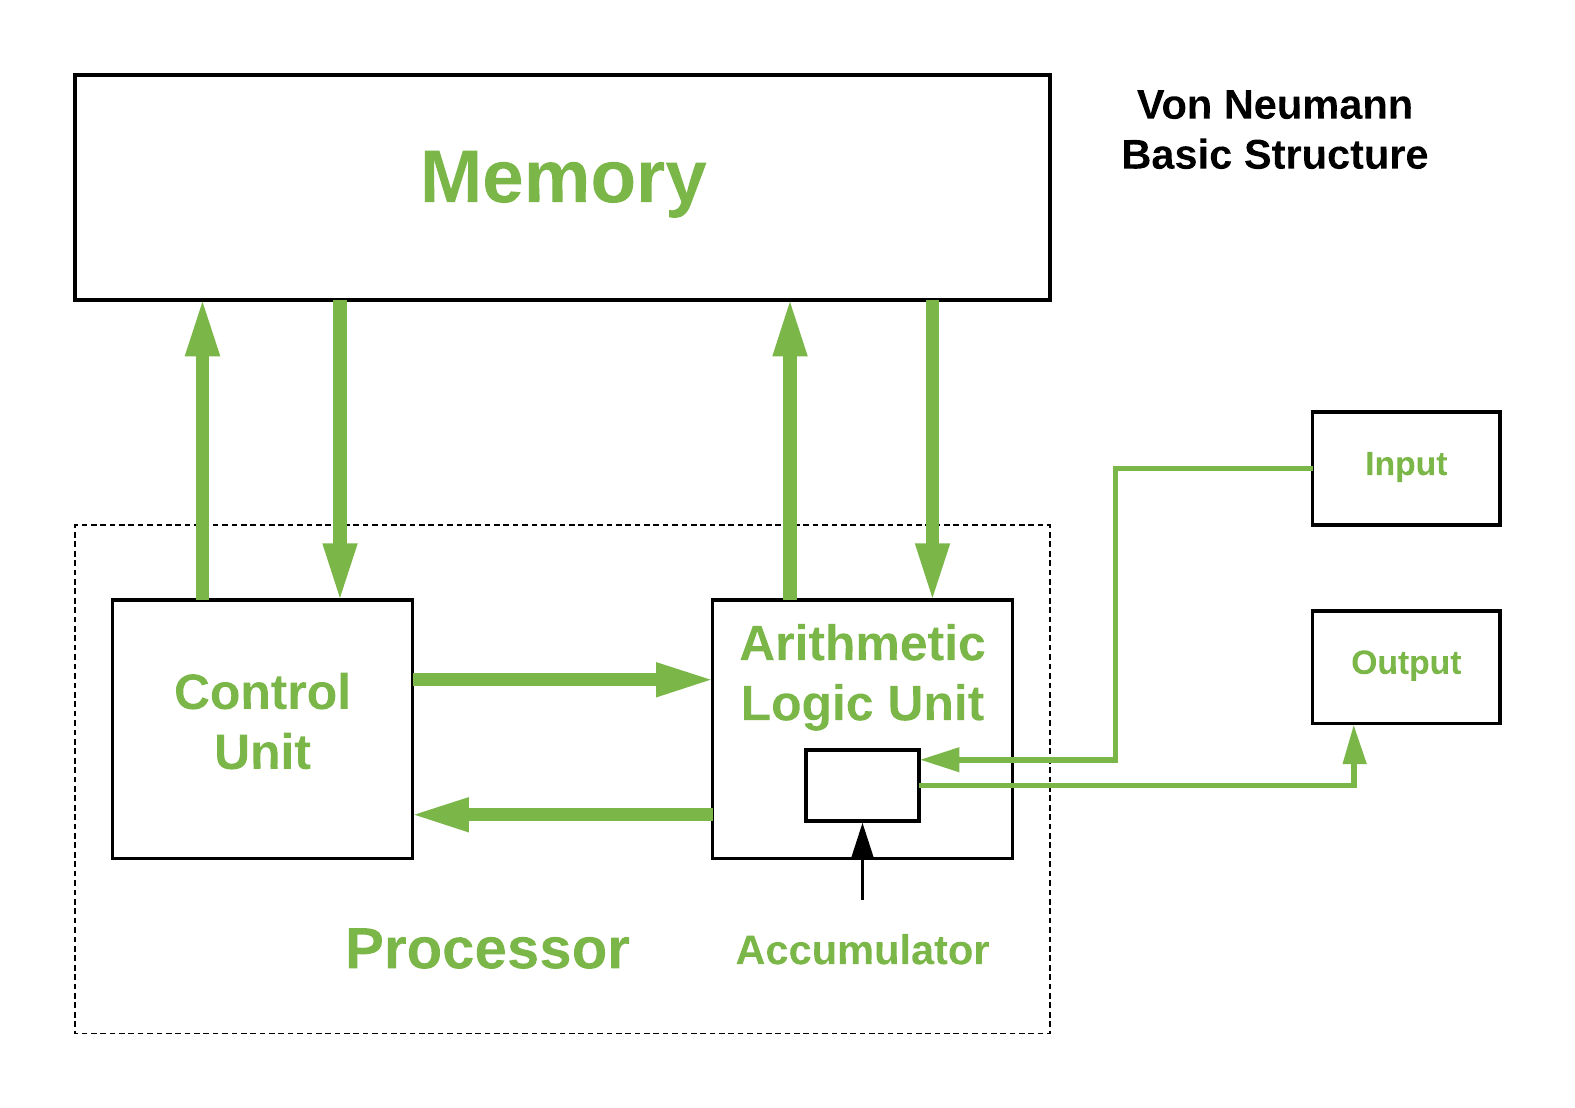
\includegraphics[width=0.5\textwidth,height=\textheight]{neumann.png}

Számítógép vásárlás szempontjából is alapvetően a CPU és a RAM határozza meg mennyire gyors a gép: minél nagyobb a CPU órajele (GHz) és minél több magja van, annál több utasítást tud végrehajtani a gép egy adott idő alatt, és minél nagyobb a RAM mérete (GB) annál több adatot tud egyszerre fejben tartani.
Talán nem ér minket meglepetésként, ha azt mondom, hogy a \emph{statisztikai számítások alapvetően RAM igényesek} (mert sok adattal dolgoznak). 16-32 GB már kell, hogy komolyabb statisztikai modelleket gyorsan tudjunk futtatni egy valós vállalati adattáblán (ami általában több, mint 1 millió rekroddal és minimum 30-40 oszloppal = változóval rendelkezik).

\section{A Pythonról általában}\label{a-pythonruxf3l-uxe1ltaluxe1ban}

Az Python a jegyzet írásakor a legnépszerűbb általános célú programozási nyelv, 2024 januárjában a \href{https://www.tiobe.com/tiobe-index/}{TIOBE index} alapján a legtöbb sor programkódot Python nyelven írják a fejlesztők.

A mi szempontunkból a Python olyan szempontból vonzó, hogy a külső kiegészítő csomagjai segítségével a valószínűségszámítás, statisztika és általánosabb adatelemzés műveletei könnyen és gyorsan elvégezhetők a segítségével. Tehát a Python használható olyan matematikai, statisztikai modellezési és elemzési feladatok elvégzésére alkalmas szkriptnyelvként, mint például az \href{https://cran.r-project.org/}{R} vagy a \href{https://www.mathworks.com/products/matlab.html}{Matlab}. A Python előnye ezekkel a nyelvekkel szemben, hogy mivel általános célú programnyelv, így a matematikai-statisztikai számítások eredményei sokkal könnyebben integrálhatók egy üzleti célú alkalmazásba, ami mondjuk felhasználói felülettel rendelkezik.
Ahogy az \emph{Előhang}ban már jeleztem, a jegyzet kimondottan a Python statisztikai és adatelemzési funkcióinak alapszintű bemutatásával foglalkozik. Tehát alkalmazást fejleszteni itt nem fogunk, a Pythont szkriptnyelvként működtetjük: elküldjük a programkódban megírt számítási igényeinket a gépállatnak, és az visszaköpi a számítások eredményeit a képernyőre, és mi egyrészt gyönyörködünk bennük, másrészt értelmezzük az eredményeket. Viszont, jó tudni, hogy a Python az eredmények további felhasználására is képes programnyelv. Ebben több, mint egy matematikusi körökben szintén népszerű R vagy Matlab. Hátránya a felsorolt nyelvekkel szemben, hogy mivel általános célú programnyelv, és nem kimondottan a matematikai-statisztikai számításokra optimalizált, így számos számítás lekódolása sokkal körülményesebb Pythonban, mint R-ben vagy Matlabban. De hát \emph{valamit valamiért}. :)

A Pythont, mi az \textbf{Anaconda keretrendszer}ből működtetjük, ami \href{https://www.anaconda.com/products/distribution}{innen letölthető}. Az Anaconda számos fejlesztőkörnyezetet biztosít a Python nyelvhez. Itt megjegyzendő, hogy a \textbf{Python és a Python fejlesztőkörnyezete nem összekeverendő!} A Python maga a programnyelv, amiben kódot írunk a számítógépünknek, hogy hajtsa végre, míg a fejlesztőkrönyezet az a program, amiben ezt a kódot megírjuk!
Mi a Python kódjainkat \textbf{Spyder fejlesztőkörnyezetben} írjuk majd, mivel ez a fejlesztőkörnyezet az, ami leginkább a Python matematikai-statisztikai műveleteket végrehajtó, szkriptnyelv-szerű használatára van optimalizálva.

Miután telepítettük és elindítottuk az Anaconda keretrendszert, a kezdőképernyőről rögtön indíthatjuk is a Spydert:


\includegraphics[width=0.8\textwidth,height=\textheight]{Anaconda.jpg}

\section{A Spyder felülete}\label{a-spyder-feluxfclete}

A Spyder fejlesztőkörnyezet indítása után az alábbihoz hasonló képernyőkép fogad minket:

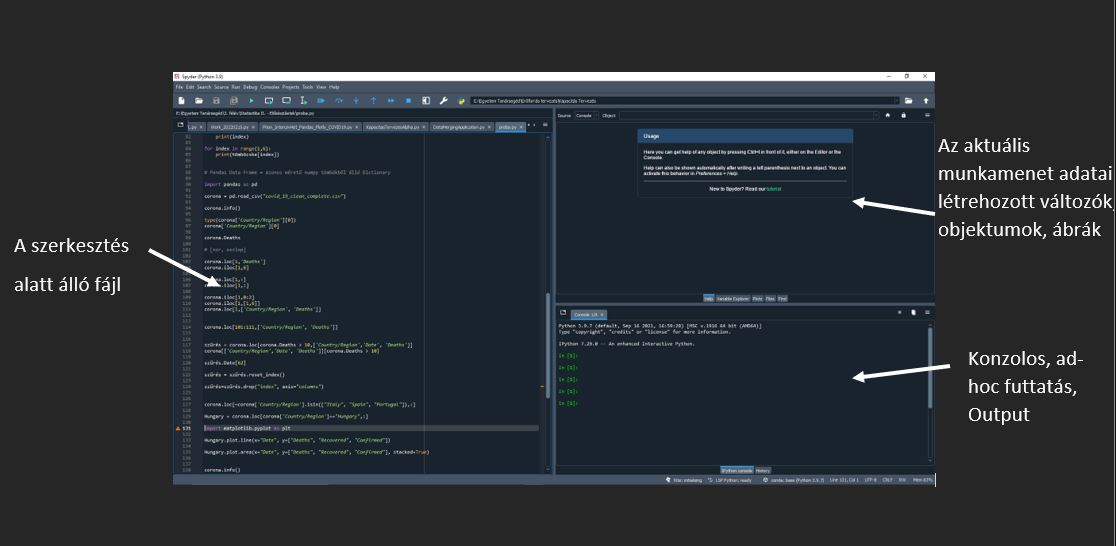
\includegraphics[width=0.9\textwidth,height=\textheight]{Spyder.jpg}

A Python kódokat a Spyder-ben \emph{.py} kiterjesztésű szkriptfájokban fogjuk írni.
Egy ilyet az alább látható módon lehet létrehozni:

A szkriptfájlba írhatjuk a gépállatnak szóló utasításainkat Python nyelven. Az utasítások végrehajtását a Spyder felület felső részén lakó 
\includegraphics{RunLine.jpg} gomb megtaposásával tudjuk kérni a géptől, aki az utasítás eredményét alul, a \emph{Console} felületen köpi ki. Ekkor a Spyder mindig azt a Python utasítást hajtja végre a gomb megnyomásakor, amiben éppen a villogó kurzorral álltunk.
Egy példában számoltassuk ki a Pythonnal, hogy mennyi \(3+2\):

Több utasítást is végre tudunk hajtatni a géppel egyszerre. Csak jelöljük ki a szkriptben a végrehajtandó utasításokat, és így kijelölés után tapossuk meg a Spyíder felső menüsorában található 
\includegraphics{RunLine.jpg} gombot!
Egy utasítást több sorba is írhatunk, de egy új utasítás mindig új sorban kezdődjön! Érdemes egy üres sort is hagyni az előző utasítás vége után!

Számoltassunk akkor most ki a Pythonnal egyszerre két dolgot is: mennyi \(3+2\) és mennyi \(3 \times 2\):

Ezek után a jegyezetek további részében a feladatok elvégzéséhez szükséges Python kódrészleteket és azok eredményét az alábbi módon jelölöm:

\begin{Shaded}
\begin{Highlighting}[]
\DecValTok{3}\OperatorTok{+}\DecValTok{2}
\end{Highlighting}
\end{Shaded}

\begin{verbatim}
## 5
\end{verbatim}

\begin{Shaded}
\begin{Highlighting}[]
\DecValTok{3}\OperatorTok{*}\DecValTok{2}
\end{Highlighting}
\end{Shaded}

\begin{verbatim}
## 6
\end{verbatim}

Ha az összes \emph{.py} fájlukban lévő kódot le szeretnénk futtatni abban a sorrendben, ahogy a fájlban szerepelnek, akkor a Spyder felső menüsorán a 
\includegraphics{RunFile.jpg} gombot kell megütni. De vigyázzunk, ilyenkor a Python nem írja ki az utasításaink eredményét a konzolra, csak akkor, ha külön beágyazzuk őket egy \texttt{print} nevű extra utasítás zárójelei közé!

\begin{Shaded}
\begin{Highlighting}[]
\BuiltInTok{print}\NormalTok{(}\DecValTok{3}\OperatorTok{+}\DecValTok{2}\NormalTok{)}
\end{Highlighting}
\end{Shaded}

\begin{verbatim}
## 5
\end{verbatim}

\begin{Shaded}
\begin{Highlighting}[]
\BuiltInTok{print}\NormalTok{(}\DecValTok{3}\OperatorTok{*}\DecValTok{2}\NormalTok{)}
\end{Highlighting}
\end{Shaded}

\begin{verbatim}
## 6
\end{verbatim}

A művelet videón:

\section{Working Directory}\label{working-directory}

Mielőtt belevágunk a Python mélyebb rejtelmeibe van még egy fontos dolog, amiről még szót kell ejteni: a \emph{Working Directory} kérdéséről.
A \emph{Working Directory} az a mappa, ahonnan a \emph{pitonállat} alapértelmezés szerint minden fájlt innen akar a memóriába tölteni és ide akar visszaírni.
A Spyder jobb felső sarkában lévő részen lehet kiválasztani és beállítani, hogy melyik mappa legyen a \emph{Working Directory}. Ezek után \textbf{minden fájlunk alapból ide fog mentődni, és minden adattáblát ide rakjunk be, amivel majd a Pythonban dolgozni akarunk!}

A Spyder-ben alapértelmezett \emph{Working Directory}-t is be tudunk állítani, ha elbandukolunk a \textbf{Tools --\textgreater{} Preferences --\textgreater{} Current working directory} menübe, és ott a \textbf{Console directory / The following directory} című résznél beállítjuk a kívánt fix mappát alapértelmezett \emph{Working Directory}-nak.

Az egész alapértelmezett \emph{Working Directory}-val kapcsolatos okfejtés működésben megnézhető a következő videón:

\section{Alapvető Python adattípusok és adatszerkezetek}\label{alapvetux151-python-adattuxedpusok-uxe9s-adatszerkezetek}

Eddig a Pythonban csak utasításokat hajtattunk végre, de a memóriában (RAM-ban) nem tároltattunk el még vele semmit.
Most itt az idő! Az utasítások eredményét a \texttt{=} szimbólummal tudjuk a memóriába valamilyen szimpatikus néven elmenteni.

\subsection{Egyszerű adattípusok}\label{egyszerux171-adattuxedpusok}

Mentsük el a 3+2 eredményét egy \texttt{összeg} névre hallgató R objektumba: \texttt{összeg\ =\ 3+2}. Az utasítás végrehajtásának hatására az \texttt{összeg} objektum megjelenik az Spyder \emph{jobb felső} sarkában lévő résznél, a \emph{Variable Explorer} fülön. (A Python alapjáraton karakterkészletben elég bő, így simán tudunk ékezetes objektumneveket is adni. De néha én a biztonság kedvéért megmaradok az ékezet nélküli elnevezéseknél. Öreg vagyok már, na! :)). A Spyder képernyőnek ezen a \emph{Variable Explorer} részén látjuk mindig azt, hogy éppen milyen Python objektumok élnek a RAM-ban:

A Python memória-objektumoknak több fajtája van. A legegyszerűbbek azok, amik csak egy értéket tartalmaznak (mint nekünk az előbb az \texttt{osszeg}). Ezeket szokás \textbf{változó}nak is hívni. Én nem szeretem ezt az elnevezést, mert keverhető a statisztikai értelemben vett változóval, ami mindig egy statisztikai megfigyelést leíró tulajdonságot/ismérvet jelent (pl. munkavállaló jövdeleme). Ennek ellenére én is gyakran használom a Python memória objektumokra a változó elnevezést. :)

A Python objektumoknak mindig van \textbf{adattípusa} is, ami \textbf{leírja, hogy az adott objektumban számértékű, szöveges, dátum vagy valami egyéb jellegű adatot tárolunk-e}. Ez azért marha fontos, mert az adattípustól függ, hogy mennyi hely szükséges a RAM-ban az objektum tárolásához. Érzésre megmondható talán, hogy egy szöveges adat tárolására több hely kell, mint egy egész szám tárolásához.

Az adattípusokat Pythonban a \texttt{type} névre hallgató \textbf{beépített függvénnyel} lehet lekérdezni.

Ezen a ponton érdemes megemlékezni arról, hogy a Pythonban léteznek \textbf{függvényként működő beépített utasítások} is. Ezek az úgynevezett Python függvények olyan utasítások, amik a matekban megszokott \(f(x)\) függvény alakot veszik fel.
A függvény neve leírja, hogy a függvény milyen műveletet végeztet el a gépállattal, és a zárójelek között pedig megadjuk, hogy milyen bemeneti paramétereken (adatokon) kell elvégezni a kijelölt műveletet. Pl. ilyen függvény volt már a \texttt{print} is.

Gyakorlati példaként lássuk akkor \textbf{Python függvények}re a \texttt{type} működését:

\begin{Shaded}
\begin{Highlighting}[]
\NormalTok{összeg }\OperatorTok{=} \DecValTok{3}\OperatorTok{+}\DecValTok{2}
\BuiltInTok{type}\NormalTok{(összeg)}
\end{Highlighting}
\end{Shaded}

\begin{verbatim}
## <class 'int'>
\end{verbatim}

Ez a \texttt{type} nevű jószág azt csiripeli nekünk, hogy ez az \texttt{összeg} című változó egy \texttt{int} adattípusú, azaz \textbf{egész szám}, leánykori angolos nevén \texttt{integer}. Tehát, ha egy Python objektum \texttt{int} adattípusú, akkor az azt jelenti, hogy ő bezony csak egész számokat tud elképzelni a világban, tört számokat nem tud tárolni.

Törtszámok tárolására vannak a \texttt{float} adattípusú objektumok.

\begin{Shaded}
\begin{Highlighting}[]
\NormalTok{tört }\OperatorTok{=} \DecValTok{3}\OperatorTok{/}\DecValTok{2}
\BuiltInTok{type}\NormalTok{(tört)}
\end{Highlighting}
\end{Shaded}

\begin{verbatim}
## <class 'float'>
\end{verbatim}

A Statisztika II. tárgyban a kétféle számítpus közti különbségnek nem igazán lesz jelentősége, de ha igazi \emph{big data}-val foglalkozik az ember, akkor a RAM takarékosság miatt számít, hogy valami csak egy egész számnyi, vagy egy törtszámnyi helyet foglal sok-sok tizedeshellyel!

Néhány egyéb fontosabb adattípus és megadási módjuk:

\begin{Shaded}
\begin{Highlighting}[]
\NormalTok{szoveg }\OperatorTok{=} \StringTok{"Hello There!"} \CommentTok{\# Figyeljünk rá, hogy szöveget a kódban csak idézőjelek közé rakjunk! Mint Excelben! :)}
\BuiltInTok{type}\NormalTok{(szoveg)}
\end{Highlighting}
\end{Shaded}

\begin{verbatim}
## <class 'str'>
\end{verbatim}

\begin{Shaded}
\begin{Highlighting}[]
\NormalTok{igazhamis }\OperatorTok{=} \VariableTok{True}
\BuiltInTok{type}\NormalTok{(igazhamis) }\CommentTok{\# a bool típusnak csak két értéke lehet: True vagy False}
\end{Highlighting}
\end{Shaded}

\begin{verbatim}
## <class 'bool'>
\end{verbatim}

A fenti kódrészletben szereplő \textbf{\#} jel a komment jele a Pythonban. A \textbf{\#} mögötti részeket a gépállat nem fogja végrehajtani, olyan lesz neki, mintha ott sem lenne. Ezzel magunknak írhatunk a Python szkriptbe hasznos megjegyzéseket.

Az egyes adattípusok között tudunk konvertálni, ha van ennek van értelme. A konverzóra függvényeket tudunk használni, amik neve kivétel nélkül megegyezik azzal a kulcsszóval, amit a \texttt{type} függvény visszaad adattípusnak. Tehát a függvény, ami mondjuk az objektumot szöveggé, azaz stringgé konvertálja az \texttt{str} névre hallgat.

Tehát akkor számból tudunk szöveget csinálni:

\begin{Shaded}
\begin{Highlighting}[]
\NormalTok{szam }\OperatorTok{=} \DecValTok{1992}
\BuiltInTok{type}\NormalTok{(szam)}
\end{Highlighting}
\end{Shaded}

\begin{verbatim}
## <class 'int'>
\end{verbatim}

\begin{Shaded}
\begin{Highlighting}[]
\NormalTok{nemszam }\OperatorTok{=} \BuiltInTok{str}\NormalTok{(szam)}
\BuiltInTok{type}\NormalTok{(nemszam)}
\end{Highlighting}
\end{Shaded}

\begin{verbatim}
## <class 'str'>
\end{verbatim}

\begin{Shaded}
\begin{Highlighting}[]
\NormalTok{nemszam}
\end{Highlighting}
\end{Shaded}

\begin{verbatim}
## '1992'
\end{verbatim}

Láthjatjuk, hogy amikor kiíratjuk a \texttt{nemszam} változót, akkor ott az \(1992\) már aposztrófok között van, ami azt jelöli, hogy ez beza már szöveges, azaz \emph{string} adat.

Olyan szövegből tudunk számot csinálni, aminek tartalma tényleg egy valid szám:

\begin{Shaded}
\begin{Highlighting}[]
\NormalTok{szöveg }\OperatorTok{=} \StringTok{"1992"}
\BuiltInTok{type}\NormalTok{(szöveg)}
\end{Highlighting}
\end{Shaded}

\begin{verbatim}
## <class 'str'>
\end{verbatim}

\begin{Shaded}
\begin{Highlighting}[]
\NormalTok{nemszöveg }\OperatorTok{=} \BuiltInTok{int}\NormalTok{(szöveg)}
\BuiltInTok{type}\NormalTok{(nemszöveg)}
\end{Highlighting}
\end{Shaded}

\begin{verbatim}
## <class 'int'>
\end{verbatim}

Tizedestörtekkel vigyázzunk! A \textbf{Python angol lokalizációt feltételez mindig}, így tizedes pontot kell alkalmazni! A tizedes vesszővel írt számot nem fogja felismerni, és hisztis hibaüzenetet dob. :( A \texttt{nemjo} változó pedig nem jön létre a memóriában.

\begin{Shaded}
\begin{Highlighting}[]
\NormalTok{nemjo }\OperatorTok{=} \BuiltInTok{float}\NormalTok{(}\StringTok{"3,14"}\NormalTok{)}
\end{Highlighting}
\end{Shaded}

\begin{verbatim}
## ValueError: could not convert string to float: '3,14'
\end{verbatim}

\begin{Shaded}
\begin{Highlighting}[]
\NormalTok{nemjo}
\end{Highlighting}
\end{Shaded}

\begin{verbatim}
## NameError: name 'nemjo' is not defined
\end{verbatim}

\begin{Shaded}
\begin{Highlighting}[]
\BuiltInTok{type}\NormalTok{(nemjo)}
\end{Highlighting}
\end{Shaded}

\begin{verbatim}
## NameError: name 'nemjo' is not defined
\end{verbatim}

De ha a törtszám tizedes ponttal adott a string változóban, akkor az minden további nélkül \texttt{float} adattípusra konvertálható.

\begin{Shaded}
\begin{Highlighting}[]
\NormalTok{jo }\OperatorTok{=} \BuiltInTok{float}\NormalTok{(}\StringTok{"3.14"}\NormalTok{)}
\NormalTok{jo}
\end{Highlighting}
\end{Shaded}

\begin{verbatim}
## 3.14
\end{verbatim}

\begin{Shaded}
\begin{Highlighting}[]
\BuiltInTok{type}\NormalTok{(jo)}
\end{Highlighting}
\end{Shaded}

\begin{verbatim}
## <class 'float'>
\end{verbatim}

Ha törtszámot (\texttt{float}) etetünk meg vacsorára az \texttt{int} függvénnyel, akkor annak az egészrészét veszi.

\begin{Shaded}
\begin{Highlighting}[]
\NormalTok{fura }\OperatorTok{=} \BuiltInTok{int}\NormalTok{(}\FloatTok{3.14}\NormalTok{)}
\NormalTok{fura}
\end{Highlighting}
\end{Shaded}

\begin{verbatim}
## 3
\end{verbatim}

\begin{Shaded}
\begin{Highlighting}[]
\BuiltInTok{type}\NormalTok{(fura)}
\end{Highlighting}
\end{Shaded}

\begin{verbatim}
## <class 'int'>
\end{verbatim}

Pythonban a rosszul beállított adattípusokból születhet pár baleset. Íme a leggyakoribb példák.

A \texttt{+} két string között az összefűzést jelenti, így az alábbi kód tökéletesen működőképes.

\begin{Shaded}
\begin{Highlighting}[]
\NormalTok{szoveg1 }\OperatorTok{=} \StringTok{"Hello"}
\NormalTok{szoveg2 }\OperatorTok{=} \StringTok{"There"}

\NormalTok{szoveg1}\OperatorTok{+}\NormalTok{szoveg2}
\end{Highlighting}
\end{Shaded}

\begin{verbatim}
## 'HelloThere'
\end{verbatim}

Viszont a string és integer összege nem értelmezhető, így hibaüzi lesz a vége\ldots mily meglepő :)
Ellenben a szorzatuk értelmes eredményt mutat: a stringet összefűzi annyiszor amennyi az integer típusú változó értéke!

\begin{Shaded}
\begin{Highlighting}[]
\NormalTok{szoveg }\OperatorTok{=} \StringTok{"3"}
\NormalTok{szam }\OperatorTok{=} \DecValTok{4}

\NormalTok{szoveg}\OperatorTok{+}\NormalTok{szam}
\end{Highlighting}
\end{Shaded}

\begin{verbatim}
## TypeError: can only concatenate str (not "int") to str
\end{verbatim}

\begin{Shaded}
\begin{Highlighting}[]
\NormalTok{szoveg}\OperatorTok{*}\NormalTok{szam}
\end{Highlighting}
\end{Shaded}

\begin{verbatim}
## '3333'
\end{verbatim}

Érdemes megnézni mi történik, ha egy stringként tárolt egész számot és egy integerként tárolt egész számot úgy ``adunk össze'' és ``szorzunk össze'', hogy előtte a stringet integerré, vagy floattá konvertáljuk.

\begin{Shaded}
\begin{Highlighting}[]
\NormalTok{szoveg }\OperatorTok{=} \StringTok{"3"}
\NormalTok{szam }\OperatorTok{=} \DecValTok{4}

\BuiltInTok{int}\NormalTok{(szoveg)}\OperatorTok{+}\NormalTok{szam}
\end{Highlighting}
\end{Shaded}

\begin{verbatim}
## 7
\end{verbatim}

\begin{Shaded}
\begin{Highlighting}[]
\BuiltInTok{int}\NormalTok{(szoveg)}\OperatorTok{*}\NormalTok{szam}
\end{Highlighting}
\end{Shaded}

\begin{verbatim}
## 12
\end{verbatim}

\begin{Shaded}
\begin{Highlighting}[]
\BuiltInTok{float}\NormalTok{(szoveg)}\OperatorTok{+}\NormalTok{szam}
\end{Highlighting}
\end{Shaded}

\begin{verbatim}
## 7.0
\end{verbatim}

\begin{Shaded}
\begin{Highlighting}[]
\BuiltInTok{float}\NormalTok{(szoveg)}\OperatorTok{*}\NormalTok{szam}
\end{Highlighting}
\end{Shaded}

\begin{verbatim}
## 12.0
\end{verbatim}

Ekkor igazából semmi galiba nem történik, minden szituáció értelmes eredményre vezet. Annyi, hogy amikor \texttt{float}-ra konvertáltuk a stringben tárolt egész számot, akkor az eredmény is \texttt{float} típusú objektum lesz. Ezt onnan látni a \texttt{type} függvény nélkül, hogy pl. a \texttt{float(szoveg)+szam} eredménye \(7.0\) lesz a \texttt{int(szoveg)+szam}-féle \(7\) helyett.

Viszont, ha a stringben egy tizedes törtet tárolok el (rendesen tizedes ponttal), akkor az már összeveszik az \texttt{int} függvénnyel, és ezekben a csillagálásokban hibát dob a pitonállat.

\begin{Shaded}
\begin{Highlighting}[]
\NormalTok{szoveg }\OperatorTok{=} \StringTok{"3.5"}
\NormalTok{szam }\OperatorTok{=} \DecValTok{4}

\NormalTok{szoveg}\OperatorTok{+}\NormalTok{szam}
\end{Highlighting}
\end{Shaded}

\begin{verbatim}
## TypeError: can only concatenate str (not "int") to str
\end{verbatim}

\begin{Shaded}
\begin{Highlighting}[]
\NormalTok{szoveg}\OperatorTok{*}\NormalTok{szam}
\end{Highlighting}
\end{Shaded}

\begin{verbatim}
## '3.53.53.53.5'
\end{verbatim}

\begin{Shaded}
\begin{Highlighting}[]
\BuiltInTok{int}\NormalTok{(szoveg)}\OperatorTok{+}\NormalTok{szam}
\end{Highlighting}
\end{Shaded}

\begin{verbatim}
## ValueError: invalid literal for int() with base 10: '3.5'
\end{verbatim}

\begin{Shaded}
\begin{Highlighting}[]
\BuiltInTok{int}\NormalTok{(szoveg)}\OperatorTok{*}\NormalTok{szam}
\end{Highlighting}
\end{Shaded}

\begin{verbatim}
## ValueError: invalid literal for int() with base 10: '3.5'
\end{verbatim}

\begin{Shaded}
\begin{Highlighting}[]
\BuiltInTok{float}\NormalTok{(szoveg)}\OperatorTok{+}\NormalTok{szam}
\end{Highlighting}
\end{Shaded}

\begin{verbatim}
## 7.5
\end{verbatim}

\begin{Shaded}
\begin{Highlighting}[]
\BuiltInTok{float}\NormalTok{(szoveg)}\OperatorTok{*}\NormalTok{szam}
\end{Highlighting}
\end{Shaded}

\begin{verbatim}
## 14.0
\end{verbatim}

Ha egészrészt szeretnék venni a stringként tárolt törtszámomból, akkor az \texttt{int} alkalmazása előtt beza \texttt{float}-tá kell konvertálni.

\begin{Shaded}
\begin{Highlighting}[]
\NormalTok{szoveg }\OperatorTok{=} \StringTok{"3.5"}
\NormalTok{szam }\OperatorTok{=} \DecValTok{4}

\NormalTok{szoveg}\OperatorTok{+}\NormalTok{szam}
\end{Highlighting}
\end{Shaded}

\begin{verbatim}
## TypeError: can only concatenate str (not "int") to str
\end{verbatim}

\begin{Shaded}
\begin{Highlighting}[]
\NormalTok{szoveg}\OperatorTok{*}\NormalTok{szam}
\end{Highlighting}
\end{Shaded}

\begin{verbatim}
## '3.53.53.53.5'
\end{verbatim}

\begin{Shaded}
\begin{Highlighting}[]
\BuiltInTok{int}\NormalTok{(}\BuiltInTok{float}\NormalTok{(szoveg))}\OperatorTok{+}\NormalTok{szam}
\end{Highlighting}
\end{Shaded}

\begin{verbatim}
## 7
\end{verbatim}

\begin{Shaded}
\begin{Highlighting}[]
\BuiltInTok{int}\NormalTok{(}\BuiltInTok{float}\NormalTok{(szoveg))}\OperatorTok{*}\NormalTok{szam}
\end{Highlighting}
\end{Shaded}

\begin{verbatim}
## 12
\end{verbatim}

\begin{Shaded}
\begin{Highlighting}[]
\BuiltInTok{float}\NormalTok{(szoveg)}\OperatorTok{+}\NormalTok{szam}
\end{Highlighting}
\end{Shaded}

\begin{verbatim}
## 7.5
\end{verbatim}

\begin{Shaded}
\begin{Highlighting}[]
\BuiltInTok{float}\NormalTok{(szoveg)}\OperatorTok{*}\NormalTok{szam}
\end{Highlighting}
\end{Shaded}

\begin{verbatim}
## 14.0
\end{verbatim}

\subsection{Összetett adatszerkezetek}\label{uxf6sszetett-adatszerkezetek}

\subsubsection{\texorpdfstring{A Python \texttt{list}}{A Python list}}\label{a-python-list}

Egyszerre több értéket tartalmazó objektumot is fel tudunk venni a Python memóriájába, ha \texttt{{[}{]}} zárójelek között vesszővel felsoroljuk az eltárolandó értékeket. Ennek az objektumnak a neve \texttt{list}.

\begin{Shaded}
\begin{Highlighting}[]
\NormalTok{sokszam }\OperatorTok{=}\NormalTok{ [}\FloatTok{3.14}\NormalTok{, }\FloatTok{2.71}\NormalTok{, }\DecValTok{88}\NormalTok{, }\DecValTok{1234}\NormalTok{]}
\BuiltInTok{type}\NormalTok{(sokszam)}
\end{Highlighting}
\end{Shaded}

\begin{verbatim}
## <class 'list'>
\end{verbatim}

Írassuk ki a teljes listát egyben az outputra!

\begin{Shaded}
\begin{Highlighting}[]
\NormalTok{sokszam}
\end{Highlighting}
\end{Shaded}

\begin{verbatim}
## [3.14, 2.71, 88, 1234]
\end{verbatim}

Kérjük le a lista \(1.\) és \(3.\) elemeit! Egy elemet a listából a sorszámával tudunk kinyerni, ha ezt a sorszámot \texttt{{[}{]}} zárójelek között megadjuk. Ugyanakkor figyeljünk, hogy a Pitonállat \(0\)-tól indexel! Azaz, az 1. elem a 0.; 2. az 1.; 3. a 2. és stb.

\begin{Shaded}
\begin{Highlighting}[]
\NormalTok{sokszam[}\DecValTok{0}\NormalTok{]}
\end{Highlighting}
\end{Shaded}

\begin{verbatim}
## 3.14
\end{verbatim}

\begin{Shaded}
\begin{Highlighting}[]
\NormalTok{sokszam[}\DecValTok{2}\NormalTok{]}
\end{Highlighting}
\end{Shaded}

\begin{verbatim}
## 88
\end{verbatim}

Nézzük meg az adattípusait is ezeknek a listaelemeknek.

\begin{Shaded}
\begin{Highlighting}[]
\BuiltInTok{type}\NormalTok{(sokszam[}\DecValTok{0}\NormalTok{])}
\end{Highlighting}
\end{Shaded}

\begin{verbatim}
## <class 'float'>
\end{verbatim}

\begin{Shaded}
\begin{Highlighting}[]
\BuiltInTok{type}\NormalTok{(sokszam[}\DecValTok{2}\NormalTok{])}
\end{Highlighting}
\end{Shaded}

\begin{verbatim}
## <class 'int'>
\end{verbatim}

Láthatjuk, hogy a lista megőrzi az elemeinek eredeti adattípusát. Tehát, a \(3.14\) adattípusa \texttt{float}, míg a \(88\)-é \texttt{int}. Ezzel sokat spórol a memóriánkon, hogy nem kényszeríti át a \(88\)-at is \texttt{float}-ba az egységesség jegyében.

Ez a logika szövegekkel is működik. Ha felveszek egy szöveges értéket is a listába, akkor annak az adattípusa string, azaz \texttt{str} lesz. A számértékű adatok pedig maradnak annak rendje és módja szerint \texttt{float} és \texttt{int} típusban, ami éppen kell. :)

\begin{Shaded}
\begin{Highlighting}[]
\NormalTok{sokszam\_sokszoveg }\OperatorTok{=}\NormalTok{ [}\DecValTok{88}\NormalTok{, }\DecValTok{42}\NormalTok{, }\StringTok{"Hello"}\NormalTok{, }\DecValTok{1992}\NormalTok{, }\DecValTok{9}\NormalTok{, }\StringTok{"There"}\NormalTok{, }\StringTok{"Friend"}\NormalTok{, }\DecValTok{11}\NormalTok{]}

\BuiltInTok{type}\NormalTok{(sokszam\_sokszoveg[}\DecValTok{0}\NormalTok{])}
\end{Highlighting}
\end{Shaded}

\begin{verbatim}
## <class 'int'>
\end{verbatim}

\begin{Shaded}
\begin{Highlighting}[]
\BuiltInTok{type}\NormalTok{(sokszam\_sokszoveg[}\DecValTok{2}\NormalTok{])}
\end{Highlighting}
\end{Shaded}

\begin{verbatim}
## <class 'str'>
\end{verbatim}

Kérjük le, hogy egy lista hány elemet tartalmaz. Ezt a \texttt{len} nevű függvény intézi nekünk.

\begin{Shaded}
\begin{Highlighting}[]
\BuiltInTok{len}\NormalTok{(sokszam\_sokszoveg)}
\end{Highlighting}
\end{Shaded}

\begin{verbatim}
## 8
\end{verbatim}

8 elemű a lista, szupszi!

Viszont, ezt az elemszám lekérdezést meg lehet oldani úgynevezett \textbf{metódus} segítségével is! A \textbf{metódusok olyan függvények, amik egy konkrét memóriában élő objektumon hajtanak végre műveleteket}. Ez a spéci logika a Python nyelvben úgy jelenik meg, hogy \textbf{nem azt mondjuk}, hogy \(f(x)\) módon végrehajtom az \(f\) műveletet az \(x\) objektumon. Mint ahogy a \texttt{len(sokszam\_sokszoveg)} is működik, **hanem úgy gondolkodunk, hogy \(x.f()\) módon végrehajtjuk az \(x\) objektumon az \(f\) műveletet.
Ez a gyakorlatban a \texttt{sokszam\_sokszoveg} nevű lista elemszámának lekérdezésénél az alábbi módon működik.

\begin{Shaded}
\begin{Highlighting}[]
\NormalTok{sokszam\_sokszoveg.}\FunctionTok{\_\_len\_\_}\NormalTok{()}
\end{Highlighting}
\end{Shaded}

\begin{verbatim}
## 8
\end{verbatim}

Királyság, az eredmény így is tök \(8\). :) A legtöbb metódus nevében amúgy nincsenek ilyen hosszas \texttt{\_\_} részek. Illetve, a metódusok zárójelei közé lehet majd egyéb paramétereket is írni, amik szabályozzák a metódus működését. Ilyen például a lista elemeinek sorbarendezési művelete.

Egy listát sorba rendezni ugyanis már csak metódussal tudunk, ami \texttt{sort} néven fut. Ezt kell elsütni a listánkon egy kis pontocskával megtámogatva.

\begin{Shaded}
\begin{Highlighting}[]
\NormalTok{sokszam.sort()}
\NormalTok{sokszam}
\end{Highlighting}
\end{Shaded}

\begin{verbatim}
## [2.71, 3.14, 88, 1234]
\end{verbatim}

Szépen növekvő sorban vannak már itt a számaink. Viszont BRÉKÓ van, mert a \texttt{sort} metódus \textbf{felülírta az eredeti listát, tehát az értékek eredeti sorrendje elveszett!} Ha \textbf{szükségünk van az eredeti sorrendre}, akkor beza \textbf{másolatot kell készíteni az eredeti listából a rendezés előtt!} Ezt a másolat készítést a \texttt{copy} metódussal tudjuk megtenni. Ha ezt nem alkalmazzuk, akkor a gépállat olyan szinten kezeli az új objektumot is, hogy mindent megcsinál vele, amit az eredetivel! Ha ezt a kapcsolatot a másolat és az eredeti objektum között \emph{el akarjuk vágni}, akkor kell a \texttt{copy} metódus.

\begin{Shaded}
\begin{Highlighting}[]
\NormalTok{sokszam }\OperatorTok{=}\NormalTok{ [}\FloatTok{3.14}\NormalTok{, }\FloatTok{2.71}\NormalTok{, }\DecValTok{1234}\NormalTok{, }\DecValTok{88}\NormalTok{]}
\NormalTok{sokszam\_copy }\OperatorTok{=}\NormalTok{ sokszam.copy()}
\NormalTok{sokszam.sort()}
\NormalTok{sokszam}
\end{Highlighting}
\end{Shaded}

\begin{verbatim}
## [2.71, 3.14, 88, 1234]
\end{verbatim}

\begin{Shaded}
\begin{Highlighting}[]
\NormalTok{sokszam\_copy}
\end{Highlighting}
\end{Shaded}

\begin{verbatim}
## [3.14, 2.71, 1234, 88]
\end{verbatim}

Láthatjuk, hogy a fenti példában minden oké, megvan az eredeti sorrend is a \texttt{sokszam\_copy}-ban. De itt lentebb, ha lehagyom a \texttt{copy}-t, akkor GázGéza van!

\begin{Shaded}
\begin{Highlighting}[]
\NormalTok{sokszam }\OperatorTok{=}\NormalTok{ [}\FloatTok{3.14}\NormalTok{, }\FloatTok{2.71}\NormalTok{, }\DecValTok{1234}\NormalTok{, }\DecValTok{88}\NormalTok{]}
\NormalTok{sokszam\_copy }\OperatorTok{=}\NormalTok{ sokszam}
\NormalTok{sokszam.sort()}
\NormalTok{sokszam}
\end{Highlighting}
\end{Shaded}

\begin{verbatim}
## [2.71, 3.14, 88, 1234]
\end{verbatim}

\begin{Shaded}
\begin{Highlighting}[]
\NormalTok{sokszam\_copy}
\end{Highlighting}
\end{Shaded}

\begin{verbatim}
## [2.71, 3.14, 88, 1234]
\end{verbatim}

Viszont, ha csökkenő és nem növekvő sorrendet akarok a listában, akkor azt a \texttt{sort} metódus zárójelei között, \textbf{paraméterként tudom megadni} \texttt{reverse=True} módon.

\begin{Shaded}
\begin{Highlighting}[]
\NormalTok{sokszam.sort(reverse}\OperatorTok{=}\VariableTok{True}\NormalTok{)}
\NormalTok{sokszam}
\end{Highlighting}
\end{Shaded}

\begin{verbatim}
## [1234, 88, 3.14, 2.71]
\end{verbatim}

Oké, ez működik! :) Azt, hogy egy metódusnak vagy általános függvénynek milyen paraméterei vannak, azt pl. a Python nyelv \href{https://www.w3schools.com/python/ref_list_sort.asp}{w3schools-on található online dokumentációjából} lehet kideríteni. Itt a metódus/függvény nevére kell rákeresni.
Szép szóval azt szokás mondani, hogy a dokumentáció megadja, hogy az egyes Python függvényeket milyen paraméterezéssel (más néven argumentumokkal) lehet \emph{meghívni}.

A sorbarendezés működik csak stringeket tartalmazó listára is.

\begin{Shaded}
\begin{Highlighting}[]
\NormalTok{soknév }\OperatorTok{=}\NormalTok{ [}\StringTok{"Kovács"}\NormalTok{, }\StringTok{"László"}\NormalTok{, }\StringTok{"Balázsné"}\NormalTok{, }\StringTok{"Mócsai"}\NormalTok{, }\StringTok{"Andrea"}\NormalTok{, }\StringTok{"Musa"}\NormalTok{]}

\NormalTok{soknév.sort()}
\NormalTok{soknév}
\end{Highlighting}
\end{Shaded}

\begin{verbatim}
## ['Andrea', 'Balázsné', 'Kovács', 'László', 'Musa', 'Mócsai']
\end{verbatim}

\begin{Shaded}
\begin{Highlighting}[]
\NormalTok{soknév.sort(reverse}\OperatorTok{=}\VariableTok{True}\NormalTok{)}
\NormalTok{soknév}
\end{Highlighting}
\end{Shaded}

\begin{verbatim}
## ['Mócsai', 'Musa', 'László', 'Kovács', 'Balázsné', 'Andrea']
\end{verbatim}

Ellenben, ha a listában vegyesen vannak stringek és valami számértéket jelölő adattípusok (\texttt{int} és \texttt{float}), akkor a rendezés vége egy szép kis hibaüzenet lesz.

\begin{Shaded}
\begin{Highlighting}[]
\NormalTok{sokszam\_sokszoveg }\OperatorTok{=}\NormalTok{ [}\DecValTok{88}\NormalTok{, }\DecValTok{42}\NormalTok{, }\StringTok{"Hello"}\NormalTok{, }\DecValTok{1992}\NormalTok{, }\DecValTok{9}\NormalTok{, }\StringTok{"There"}\NormalTok{, }\StringTok{"Friend"}\NormalTok{, }\DecValTok{11}\NormalTok{]}
\NormalTok{sokszam\_sokszoveg.sort()}
\end{Highlighting}
\end{Shaded}

\begin{verbatim}
## TypeError: '<' not supported between instances of 'str' and 'int'
\end{verbatim}

Na ezt a rendezősdit vegyes adattípusokon már tényleg nem érti a gépállat!
Tanulság: rendezés esetén nem iszunk kevertet! :)

Nézzük meg hogyan tudunk több, mint 1 elemet kiválasztani a listákból!

Kérjünk le minden elemet 2-től 4-ig. Ezt úgy tudjuk megtenni, hogy a lista neve után \texttt{{[}{]}} zárójelek között \texttt{:}-tal elválasztva megadjuk a kiválasztás kezdeti és végső sorszámát: \texttt{kezdet:vége}. Azonban \textbf{vigyázzunk!} A \textbf{kezdeti végpontot zárt, a végsőt nyílt} intervallumként értelmezi a Pitonállat! Tehát ennek szellemében, ha figyelembe vesszük a \(0\)-val kezdődő indexszálást is, akkor a 2-től 4-ig tartó listaelemeket \texttt{(2-1):4\ =\ 1:4} módon kell megadni.

\begin{Shaded}
\begin{Highlighting}[]
\NormalTok{sokszam\_sokszoveg[}\DecValTok{1}\NormalTok{:}\DecValTok{4}\NormalTok{]}
\end{Highlighting}
\end{Shaded}

\begin{verbatim}
## [42, 'Hello', 1992]
\end{verbatim}

A hecc kedvéért nézzük meg mit ad vissza gépállat, ha nem létező elemet kérünk le.

\begin{Shaded}
\begin{Highlighting}[]
\NormalTok{sokszam\_sokszoveg[}\DecValTok{9}\NormalTok{]}
\end{Highlighting}
\end{Shaded}

\begin{verbatim}
## IndexError: list index out of range
\end{verbatim}

Csak, hogy emlékezzünk arra, hogy az \texttt{IndexError:\ list\ index\ out\ of\ range} hibaüzenet nem létező listelem kiválasztását jelenti. :)

\subsubsection{\texorpdfstring{A Python \texttt{Dictionary}}{A Python Dictionary}}\label{a-python-dictionary}

A Python \texttt{Dictionary} típusú (\texttt{dict}) objektuma nemes egyszerűséggel egy olyan \texttt{list}, amiben \textbf{szöveges kulcsokkal és nem sorszámmal indexeljük a listaelemeket}.

Létrehozni az értékek és a szöveges azonosítók (azaz kulcsok) megadásával tudjuk \texttt{"kulcs"\ :\ "érték"} módon \texttt{\{\}} zárójelek között.

Hozzunk létre egy \texttt{Laci} nevű \texttt{dict}-et, ami tartalmazza Laci 3 legfontosabb ismérvét: vezeték- és keresztnevét, valamint születési évét.

\begin{Shaded}
\begin{Highlighting}[]
\NormalTok{Laci }\OperatorTok{=}\NormalTok{ \{}\StringTok{"vezetek"}\NormalTok{: }\StringTok{"Kovács"}\NormalTok{,}
\StringTok{"kereszt"}\NormalTok{: }\StringTok{"László"}\NormalTok{,}
\StringTok{"year"}\NormalTok{: }\DecValTok{1992}\NormalTok{\}}
\NormalTok{Laci}
\end{Highlighting}
\end{Shaded}

\begin{verbatim}
## {'vezetek': 'Kovács', 'kereszt': 'László', 'year': 1992}
\end{verbatim}

\begin{Shaded}
\begin{Highlighting}[]
\BuiltInTok{type}\NormalTok{(Laci)}
\end{Highlighting}
\end{Shaded}

\begin{verbatim}
## <class 'dict'>
\end{verbatim}

Kérjük le a 2. elemet a szótárból.

\begin{Shaded}
\begin{Highlighting}[]
\NormalTok{Laci[}\DecValTok{1}\NormalTok{]}
\end{Highlighting}
\end{Shaded}

\begin{verbatim}
## KeyError: 1
\end{verbatim}

Teljesen jogosan nyávog a pitonkénk, hogy ezt nem érti, hiszen itt a 2. elem nem értelmezhető, mivel nem sorszámmal azonosíthatók a szótár elemei.

De ezt az alábbi hivatkozást a szöveges kulcson keresztül érteni fogja.

\begin{Shaded}
\begin{Highlighting}[]
\NormalTok{Laci[}\StringTok{"kereszt"}\NormalTok{]}
\end{Highlighting}
\end{Shaded}

\begin{verbatim}
## 'László'
\end{verbatim}

Milyenek az adattípusok?

\begin{Shaded}
\begin{Highlighting}[]
\BuiltInTok{type}\NormalTok{(Laci[}\StringTok{"vezetek"}\NormalTok{])}
\end{Highlighting}
\end{Shaded}

\begin{verbatim}
## <class 'str'>
\end{verbatim}

\begin{Shaded}
\begin{Highlighting}[]
\BuiltInTok{type}\NormalTok{(Laci[}\StringTok{"kereszt"}\NormalTok{])}
\end{Highlighting}
\end{Shaded}

\begin{verbatim}
## <class 'str'>
\end{verbatim}

\begin{Shaded}
\begin{Highlighting}[]
\BuiltInTok{type}\NormalTok{(Laci[}\StringTok{"year"}\NormalTok{])}
\end{Highlighting}
\end{Shaded}

\begin{verbatim}
## <class 'int'>
\end{verbatim}

Nagyszerű! Mint a listában, minden elem őrzi szépen az eredeti adattípusát. :)

\subsection{\texorpdfstring{A \texttt{numpy} tömb}{A numpy tömb}}\label{a-numpy-tuxf6mb}

Nekünk azért jó, mert úgy van optimalizálva ez az adatszerkezet, hogy az elemein a \textbf{statisztikai számítások} (átlag, medián, szórás, stb.) \textbf{nagy adattömegen is gyorsan} fussanak!

Ehhez már külön csomag kell, ami \texttt{numpy} névre hallgat.

Külső csomagokat a Pythonhoz a \texttt{pip\ install} utasítás segítségével tudunk telepíteni. A \texttt{numpy} csomagot tehát a következő kóddal lehet felvarázsolni Pitonkánknak.

\begin{Shaded}
\begin{Highlighting}[]
\NormalTok{pip install numpy}
\end{Highlighting}
\end{Shaded}

Ezt a \textbf{fenti kódot csak egyszer kell lefutatni}, utána a Python mindig \textbf{emlékezni fog van már neki egy \texttt{numpy} névre hallgató kiegészítő csomagja}.

Viszont, a \textbf{következő kódot mindig futtassuk le mielőtt egy kódban a \texttt{numpy} csomagot használni akarjuk!}

\begin{Shaded}
\begin{Highlighting}[]
\ImportTok{import}\NormalTok{ numpy }\ImportTok{as}\NormalTok{ np}
\end{Highlighting}
\end{Shaded}

Minden \texttt{numpy} függvényt a fenti kódsor miatt egy \texttt{np} előtaggal tudunk majd csak használni. Szakkifejezéssel élve, a fenti kódsorral a \texttt{numpy} függvényeket az \texttt{np} \textbf{névtér}be töltöttük be a gépállat számára \emph{úgymond}.

Hozzunk is létre \texttt{numpy} tömböt! Ezt úgy tudjuk megtenni, hogy egy \texttt{{[}{]}} zárójelekkel létrehozott listát berakunk egy az \texttt{np} névtérben lakó \texttt{array} nevű függvény zárójelei közé.

\begin{Shaded}
\begin{Highlighting}[]
\NormalTok{tömböcske }\OperatorTok{=}\NormalTok{ np.array([}\FloatTok{3.14}\NormalTok{, }\FloatTok{2.67}\NormalTok{, }\DecValTok{88}\NormalTok{, }\DecValTok{1234}\NormalTok{])}
\BuiltInTok{type}\NormalTok{(tömböcske)}
\end{Highlighting}
\end{Shaded}

\begin{verbatim}
## <class 'numpy.ndarray'>
\end{verbatim}

\begin{Shaded}
\begin{Highlighting}[]
\NormalTok{tömböcske}
\end{Highlighting}
\end{Shaded}

\begin{verbatim}
## array([   3.14,    2.67,   88.  , 1234.  ])
\end{verbatim}

Láthatjuk is, hogy a \texttt{tömböcske} adattípusa \texttt{numpy}-féle \texttt{ndarray}, azaz tömb. :)

Egy \texttt{numpy} tömböt amúgy lehet már létező listából történő klónozással is létrehozni, szintén az \texttt{np.array} függvénnyel.

\begin{Shaded}
\begin{Highlighting}[]
\NormalTok{sokszam }\OperatorTok{=}\NormalTok{ [}\FloatTok{3.14}\NormalTok{, }\FloatTok{2.67}\NormalTok{, }\DecValTok{88}\NormalTok{, }\DecValTok{1234}\NormalTok{]}
\NormalTok{tömböcske }\OperatorTok{=}\NormalTok{ np.array(sokszam)}
\BuiltInTok{type}\NormalTok{(tömböcske)}
\end{Highlighting}
\end{Shaded}

\begin{verbatim}
## <class 'numpy.ndarray'>
\end{verbatim}

\begin{Shaded}
\begin{Highlighting}[]
\NormalTok{tömböcske}
\end{Highlighting}
\end{Shaded}

\begin{verbatim}
## array([   3.14,    2.67,   88.  , 1234.  ])
\end{verbatim}

Az elemek kiválasztása szerencsénkre ugyanúgy megy, mint \texttt{list}-ben.

Pl. az első és negyedik elemek lekérdezése az alábbi.

\begin{Shaded}
\begin{Highlighting}[]
\NormalTok{tömböcske[}\DecValTok{0}\NormalTok{]}
\end{Highlighting}
\end{Shaded}

\begin{verbatim}
## 3.14
\end{verbatim}

\begin{Shaded}
\begin{Highlighting}[]
\NormalTok{tömböcske[}\DecValTok{3}\NormalTok{]}
\end{Highlighting}
\end{Shaded}

\begin{verbatim}
## 1234.0
\end{verbatim}

Másodiktól Negyedik elemig történő kiválasztás.

\begin{Shaded}
\begin{Highlighting}[]
\NormalTok{tömböcske[}\DecValTok{1}\NormalTok{:}\DecValTok{4}\NormalTok{]}
\end{Highlighting}
\end{Shaded}

\begin{verbatim}
## array([   2.67,   88.  , 1234.  ])
\end{verbatim}

És itt olyat is lehet, hogy csak a 2. és 4. elemet szedjük ki! A sima \texttt{list} ezt pl. nem igazán tudja! Ehhez az kell, hogy a kiválasztott sorszámokat egy \texttt{list}-ként, \texttt{{[}{]}} zárójelekkel létrehozva adjuk meg az indexszeléshez használt szögletes zárójelek között!

\begin{Shaded}
\begin{Highlighting}[]
\NormalTok{tömböcske[[}\DecValTok{1}\NormalTok{,}\DecValTok{3}\NormalTok{]]}
\end{Highlighting}
\end{Shaded}

\begin{verbatim}
## array([   2.67, 1234.  ])
\end{verbatim}

Tehát, a fenti példában azért van \texttt{{[}{[}{]}{]}} használat, mert a külső \texttt{{[}{]}} a tömb indexelése miatt van, a belső \texttt{{[}{]}} pedig a kiválasztott sorszámok listája miatt kerül a képbe.

De mik itt az egyes elemek adattípusai? Lessük meg őket!

\begin{Shaded}
\begin{Highlighting}[]
\NormalTok{tömböcske[}\DecValTok{0}\NormalTok{]}
\end{Highlighting}
\end{Shaded}

\begin{verbatim}
## 3.14
\end{verbatim}

\begin{Shaded}
\begin{Highlighting}[]
\NormalTok{tömböcske[}\DecValTok{3}\NormalTok{]}
\end{Highlighting}
\end{Shaded}

\begin{verbatim}
## 1234.0
\end{verbatim}

\begin{Shaded}
\begin{Highlighting}[]
\BuiltInTok{type}\NormalTok{(tömböcske[}\DecValTok{0}\NormalTok{])}
\end{Highlighting}
\end{Shaded}

\begin{verbatim}
## <class 'numpy.float64'>
\end{verbatim}

\begin{Shaded}
\begin{Highlighting}[]
\BuiltInTok{type}\NormalTok{(tömböcske[}\DecValTok{3}\NormalTok{])}
\end{Highlighting}
\end{Shaded}

\begin{verbatim}
## <class 'numpy.float64'>
\end{verbatim}

\textbf{BRÉKÓ! A \texttt{numpy} tömbök elemeinek mindig azonos adattípusúnak kell lenniük!} Ha alapból nem azok, akkor a gépállat átkonvertál mindent a legáltalánosabb adattípusra. Az \texttt{int}ek és \texttt{float}ok esetében ez a törtszámokat is elviselő \texttt{float}.

Ellenben ha van szöveg is a dologban\ldots{}

\begin{Shaded}
\begin{Highlighting}[]
\NormalTok{szöveges\_tömb }\OperatorTok{=}\NormalTok{ np.array(sokszam\_sokszoveg)}
\BuiltInTok{type}\NormalTok{(szöveges\_tömb)}
\end{Highlighting}
\end{Shaded}

\begin{verbatim}
## <class 'numpy.ndarray'>
\end{verbatim}

\begin{Shaded}
\begin{Highlighting}[]
\NormalTok{szöveges\_tömb}
\end{Highlighting}
\end{Shaded}

\begin{verbatim}
## array(['88', '42', 'Hello', '1992', '9', 'There', 'Friend', '11'],
##       dtype='<U11')
\end{verbatim}

\begin{Shaded}
\begin{Highlighting}[]
\BuiltInTok{type}\NormalTok{(szöveges\_tömb[}\DecValTok{0}\NormalTok{])}
\end{Highlighting}
\end{Shaded}

\begin{verbatim}
## <class 'numpy.str_'>
\end{verbatim}

\begin{Shaded}
\begin{Highlighting}[]
\BuiltInTok{type}\NormalTok{(szöveges\_tömb[}\DecValTok{2}\NormalTok{])}
\end{Highlighting}
\end{Shaded}

\begin{verbatim}
## <class 'numpy.str_'>
\end{verbatim}

\ldots akkor bizony a legáltalánosabb adattípus, amit minden elem megörököl az a string, vagyis \texttt{str}!

\section{Vezérlési szerkezetek}\label{vezuxe9rluxe9si-szerkezetek}

\subsection{\texorpdfstring{Elágazás (\texttt{if})}{Elágazás (if)}}\label{eluxe1gazuxe1s-if}

Az elágazások arra az esetre vannak, ha \textbf{bizonyos utasításokat a kódunkban csak akkor akarunk végrehajtani, ha előtte valamiféle logikai feltétel teljesül}.

Például, ha egy egész szám nagyobb, mint \(10\) kiírjuk, hogy `\emph{Hatalmas}'.

Vagyis létrehozunk egy új változót \texttt{szam} néven, megnézzük, hogy az értéke nagyobb-e mint \(10\), és ha igen, akkor egy \texttt{print} függvénnyel kiírjuk tényleg a `\emph{Hatalmas}' szócskát.
Mindez Pitonul az alábbi módon néz ki.

\begin{Shaded}
\begin{Highlighting}[]
\NormalTok{szam }\OperatorTok{=} \DecValTok{13}

\ControlFlowTok{if}\NormalTok{ szam }\OperatorTok{\textgreater{}} \DecValTok{10}\NormalTok{:}
  \BuiltInTok{print}\NormalTok{(}\StringTok{"Hatalmas"}\NormalTok{)}
\end{Highlighting}
\end{Shaded}

\begin{verbatim}
## Hatalmas
\end{verbatim}

Mivel a számunk \(13\) volt, és \(13>10\), így ki lett írva, hogy `\emph{Hatalmas}'. De ha a számnak \(8\)-at adunk meg, akkor értelemszerűen nincs kiírás.

\begin{Shaded}
\begin{Highlighting}[]
\NormalTok{szam }\OperatorTok{=} \DecValTok{8}

\ControlFlowTok{if}\NormalTok{ szam }\OperatorTok{\textgreater{}} \DecValTok{10}\NormalTok{:}
  \BuiltInTok{print}\NormalTok{(}\StringTok{"Hatalmas"}\NormalTok{)}
\end{Highlighting}
\end{Shaded}

Azt figyeljük meg a fenti két kódrészletben, hogy a vizsgálandó logikai feltételt egy \texttt{if} kulcsszóval adjuk meg, majd utána egy \texttt{:}-ot írunk, és a feltétel esetén futtatandó kódot egy TAB billentyűs behúzással kezdjük a következő sorban.

\textbf{Figyelem!} Ha \textbf{nincs behúzás, akkor a pitonka mindenképp végrehajtja az utasítást, ami következik} az \texttt{if}-el kezdődő sor után!

\begin{Shaded}
\begin{Highlighting}[]
\NormalTok{szam }\OperatorTok{=} \DecValTok{8}

\ControlFlowTok{if}\NormalTok{ szam }\OperatorTok{\textgreater{}} \DecValTok{10}\NormalTok{:}
  \BuiltInTok{print}\NormalTok{(}\StringTok{"Hatalmas"}\NormalTok{)}

\BuiltInTok{print}\NormalTok{(}\StringTok{"Ezt mindenképp kiírjuk!"}\NormalTok{)}
\end{Highlighting}
\end{Shaded}

\begin{verbatim}
## Ezt mindenképp kiírjuk!
\end{verbatim}

Még olyat is tudunk csinálni egy \texttt{else} kulcsszóval, hogy ha az \texttt{if}-ben megadott logikai feltétel nem teljesül akkor is kiírunk valamit. Pl. most a feltétel nem teljesülése esetén írjuk ki azt, hogy `\emph{Törpe}'

\begin{Shaded}
\begin{Highlighting}[]
\NormalTok{szam }\OperatorTok{=} \DecValTok{3}

\ControlFlowTok{if}\NormalTok{ szam }\OperatorTok{\textgreater{}} \DecValTok{10}\NormalTok{:}
  \BuiltInTok{print}\NormalTok{(}\StringTok{"Hatalmas"}\NormalTok{)}
\ControlFlowTok{else}\NormalTok{:}
  \BuiltInTok{print}\NormalTok{(}\StringTok{"Törpe"}\NormalTok{)}
\end{Highlighting}
\end{Shaded}

\begin{verbatim}
## Törpe
\end{verbatim}

\begin{Shaded}
\begin{Highlighting}[]
\BuiltInTok{print}\NormalTok{(}\StringTok{"Ezt mindenképp kiírjuk!"}\NormalTok{)}
\end{Highlighting}
\end{Shaded}

\begin{verbatim}
## Ezt mindenképp kiírjuk!
\end{verbatim}

Ahogy a fenti kódrészlet eredménye is mutatja, \textbf{az \texttt{else} esetén is kell a behúzás az egyéb esetben végrehajtandó kódokhoz}, hogy azt csinálja nekünk a pitonállat, amit szeretnénk.

Az elvégezhető logikai összehasonlítő műveletek az \texttt{if} feltételekben egy \texttt{a} és \texttt{b} objektum között a következők a Python nyelvén:

\begin{itemize}
\tightlist
\item
  Egyenlő: \texttt{a\ ==\ b}
\item
  Nem egyenlő: \texttt{a\ !=\ b}
\item
  Kisebb: \texttt{a\ \textless{}\ b}
\item
  Nagyobb: \texttt{a\ \textgreater{}\ b}
\item
  Legalább: \texttt{a\ \textless{}=\ b}
\item
  Legfeljebb: \texttt{a\ \textgreater{}=\ b}
\end{itemize}

Az \emph{egyenlő} és \emph{nem egyenlő} természetesen működik \texttt{str}-ek esetében is, a többi viszont csak \texttt{int} és \texttt{float} adattípusú objektumokra értelmes, amúgy \emph{hibára futnak}.

\subsection{\texorpdfstring{Ciklusok (\texttt{for})}{Ciklusok (for)}}\label{ciklusok-for}

Alapvetően többféle ciklus van a programnyelvekben, de minekünk igazából csak a \texttt{for} ciklusra lesz szükségünk.

A \texttt{for} ciklus egy általunk éppen \texttt{aktualis\_elem}-nek elnevezett objektumot pörget végig egy lista vagy \texttt{numpy} tömb minden elemén. Ezzel így ki tudjuk olvasni egyesével egy tömb vagy lista minden értékét. A ``\emph{végigpörgetés}'' alias ``\emph{ciklizálás}'' során végrehajtandó kódot hívjuk \textbf{ciklusmag}nak, és ezt a kódrészletet az \texttt{if}-hez hasonló módon \textbf{behúzással kell elválasztani} a kód többi részétől!

Lássuk hát a dolgot akció közben!

\begin{Shaded}
\begin{Highlighting}[]
\NormalTok{sokszam\_sokszoveg }\OperatorTok{=}\NormalTok{ [}\DecValTok{88}\NormalTok{, }\DecValTok{42}\NormalTok{, }\StringTok{"Hello"}\NormalTok{, }\DecValTok{1992}\NormalTok{, }\DecValTok{9}\NormalTok{, }\StringTok{"There"}\NormalTok{, }\StringTok{"Friend"}\NormalTok{, }\DecValTok{11}\NormalTok{]}

\NormalTok{tömböcske }\OperatorTok{=}\NormalTok{ np.array([}\FloatTok{3.14}\NormalTok{, }\FloatTok{2.67}\NormalTok{, }\DecValTok{88}\NormalTok{, }\DecValTok{1234}\NormalTok{])}

\ControlFlowTok{for}\NormalTok{ aktualis\_elem }\KeywordTok{in}\NormalTok{ sokszam\_sokszoveg:}
\NormalTok{  aktualis\_elem}
\end{Highlighting}
\end{Shaded}

\begin{verbatim}
## 88
## 42
## 'Hello'
## 1992
## 9
## 'There'
## 'Friend'
## 11
\end{verbatim}

\begin{Shaded}
\begin{Highlighting}[]
\BuiltInTok{print}\NormalTok{(}\StringTok{"{-}{-}{-}{-}{-}{-}{-}{-}{-}{-}{-}{-}{-}{-}"}\NormalTok{)}
\end{Highlighting}
\end{Shaded}

\begin{verbatim}
## --------------
\end{verbatim}

\begin{Shaded}
\begin{Highlighting}[]
\ControlFlowTok{for}\NormalTok{ aktualis\_elem }\KeywordTok{in}\NormalTok{ tömböcske:}
\NormalTok{  aktualis\_elem}
\end{Highlighting}
\end{Shaded}

\begin{verbatim}
## 3.14
## 2.67
## 88.0
## 1234.0
\end{verbatim}

Egy \texttt{range} keresztségű függvénnyel bármilyen számsorozatot is ki tudunk íratni egy \texttt{for} ciklusban. Csak arra figyeljünk, hogy ez a függvény is 0-tól kezdi a léptetést, mint a listák és a tömbök! :).

Írjuk ki az egész számokat \(0\)-tól \(5\)-ig\ldots ehhez a \texttt{range} függvénybe \(6\)-ot kell írni paraméternek!

\begin{Shaded}
\begin{Highlighting}[]
\ControlFlowTok{for}\NormalTok{ aktualis\_elem }\KeywordTok{in} \BuiltInTok{range}\NormalTok{(}\DecValTok{6}\NormalTok{):}
\NormalTok{  aktualis\_elem}
\end{Highlighting}
\end{Shaded}

\begin{verbatim}
## 0
## 1
## 2
## 3
## 4
## 5
\end{verbatim}

Minden egész szám kiíratása \(2\)-től \(8\)-ig az alábbi módon lehetséges. Itt a \texttt{range}-ben is a felső határ egy nyílt intervallumként megadható, mint a listaelemek \texttt{:}-os kiolvasása esetén (5.2.1. fejezet).

\begin{Shaded}
\begin{Highlighting}[]
\ControlFlowTok{for}\NormalTok{ aktualis\_elem }\KeywordTok{in} \BuiltInTok{range}\NormalTok{(}\DecValTok{2}\NormalTok{,}\DecValTok{9}\NormalTok{):}
\NormalTok{  aktualis\_elem}
\end{Highlighting}
\end{Shaded}

\begin{verbatim}
## 2
## 3
## 4
## 5
## 6
## 7
## 8
\end{verbatim}

Tömb elemeit ezzel a \texttt{range} függvénnyel kiolvashatjuk a cikluson belül a sorszámuk (indexszük) segítségével is akár.

\begin{Shaded}
\begin{Highlighting}[]
\NormalTok{elemszám }\OperatorTok{=} \BuiltInTok{len}\NormalTok{(sokszam)}

\ControlFlowTok{for}\NormalTok{ aktualis\_index }\KeywordTok{in} \BuiltInTok{range}\NormalTok{(elemszám):}
\NormalTok{  sokszam[aktualis\_index]}
\end{Highlighting}
\end{Shaded}

\begin{verbatim}
## 3.14
## 2.67
## 88
## 1234
\end{verbatim}

De remélem érezzük, hogy ez kellően körülményes megoldás ahhoz képest, mintha közvetlenül a tömböt járnánk be a ciklussal. :)

\section{A Pandas data frame objektum}\label{a-pandas-data-frame-objektum}

Adattáblákat Pythonban \texttt{pandas} csomag \textbf{data frame} struktúrájában kezeljük!

Ezt, mint külön csomagot egyszer telepíteni kell.

\begin{Shaded}
\begin{Highlighting}[]
\NormalTok{pip install pandas}
\end{Highlighting}
\end{Shaded}

Aztán minden kódunk elején behivatkozni, ha használni akarjuk.

\begin{Shaded}
\begin{Highlighting}[]
\ImportTok{import}\NormalTok{ pandas }\ImportTok{as}\NormalTok{ pd}
\end{Highlighting}
\end{Shaded}

Adatvizualizációhoz a \texttt{pandas} csomaggal együttműködni képes \texttt{matplotlib} csomagra lesz szükség.

Itt is egyszer telepíteni kell.

\begin{Shaded}
\begin{Highlighting}[]
\NormalTok{pip install matplotlib}
\end{Highlighting}
\end{Shaded}

Aztán minden kódunk elején behivatkozzuk, ahol használni akarjuk.

\begin{Shaded}
\begin{Highlighting}[]
\ImportTok{import}\NormalTok{ matplotlib.pyplot }\ImportTok{as}\NormalTok{ plt}
\end{Highlighting}
\end{Shaded}

Itt is figyeljünk a \textbf{névterekre}, amikbe elraktuk a csomagok függvényeit!

Ezen a ponton jegyezném meg, hogy a \texttt{pandas} csomag olyan hatalmas, hogy függvényeinek és metódusainak \href{https://pandas.pydata.org/docs/reference/index.html}{külön dokumentációja érhető el}. \textbf{Ha egy függvény vagy metódus használatakor elakad az ember, érdemes először ebben a dokumentációban utána nézni a proglémás cucc működésének!}

Olvassuk be a covid\_19\_clean\_complete.csv fájlt, és tároljuk le az adatait egy \textbf{corona} nevű Pandas data frame-ben!

Az adatfájl egy WHO által készített historikus kimutatás a COVID-19 vírus esetszámairól a Föld országaiban 2020. április 30-cal bezárólag.

A \texttt{pandas} data frame-ekbe a legkönnyebben talán \textbf{csv} kiterjesztésű állományként tárolt adattáblákat lehet beolvasni a \texttt{read\_csv} függvény segítségével. A \textbf{csv} állományok valójában olyan \textbf{txt} fájlok, amikben egy táblázat szerepel úgy, hogy az oszlophatárokat \textbf{vesszők} jelzik! Innen is a név: \emph{comma separated values = csv}

\textbf{Figyelem!} Az alábbi beolvasó kód csak akkor működik, ha a \emph{csv} fájlt az aktuálisan beállított \textbf{Working Directory}-ba másoltuk be!!

\begin{Shaded}
\begin{Highlighting}[]
\NormalTok{corona }\OperatorTok{=}\NormalTok{ pd.read\_csv(}\StringTok{\textquotesingle{}covid\_19\_clean\_complete.csv\textquotesingle{}}\NormalTok{)}
\end{Highlighting}
\end{Shaded}

A \textbf{data frame} logikailag úgy kezelhető, mint egy \textbf{numpy tömbökből álló lista, de a listaelemeket névvel is tudjuk azonosítani, mint egy Dictionary-ben}!! Ezek a \textbf{listaelem nevek az oszlopok = változók = ismérvek nevei}! Gondoljunk bele, hogy ez mennyire logikus, hiszen a \texttt{numpy} tömbök elemeire vonatkozó azonos adattípus követelmény megfeleltethető a statisztikai ismérvek mérési skáláinak fogalmával!

Az előző bekezdésben írtakból kifolyólag a betöltendő \emph{csv} fájjal szemben vannak a \texttt{pandas} csomagnak fontos előkövetelményei:

\begin{itemize}
\tightlist
\item
  az oszlopok vesszővel elválasztottak
\item
  a tört számok tizedes pontot használnak
\item
  a szöveges adatok idézőjelek között vannak
\end{itemize}

Ha angol nyelvű oldalról töltünk le adatokat \emph{csv}-ben (pl. \href{https://www.kaggle.com/}{Kaggle}), akkor a fenti követelményeknek szinte biztosan meg fognak felelni.
Rosszul viselkedő \emph{csv}-k esetén pedig a \texttt{read\_csv} függvény különböző paramétereivel kezelhetők a problémák (tizedespont vs tizedes vessző pl.). Részletek a függvény \href{https://pandas.pydata.org/docs/reference/api/pandas.read_csv.html}{dokumentációjában}.

A beolvasandó adattáblától a \texttt{pandas} elvárja azt a logikai felépítést, hogy a tábla soraiban legyenek a statisztikai megfigyelési egységeink (emberek, országok, lakások, autók stb.) és az oszlopokban pedig a megfigyeléseket leíró tulajdonságok, azaz változók (ember kora, ország GDP-je, autó márkája stb.).

Nézzük meg ezt az adatstruktúrát a \textbf{data frame} \texttt{info} metódusának segítségével!

\begin{Shaded}
\begin{Highlighting}[]
\NormalTok{corona.info()}
\end{Highlighting}
\end{Shaded}

\begin{verbatim}
## <class 'pandas.core.frame.DataFrame'>
## RangeIndex: 26400 entries, 0 to 26399
## Data columns (total 8 columns):
##  #   Column          Non-Null Count  Dtype  
## ---  ------          --------------  -----  
##  0   Province/State  8000 non-null   object 
##  1   Country/Region  26400 non-null  object 
##  2   Lat             26400 non-null  float64
##  3   Long            26400 non-null  float64
##  4   Date            26400 non-null  object 
##  5   Confirmed       26400 non-null  int64  
##  6   Deaths          26400 non-null  int64  
##  7   Recovered       26400 non-null  int64  
## dtypes: float64(2), int64(3), object(3)
## memory usage: 1.6+ MB
\end{verbatim}

Itt tehát úgy néz ki, hogy \emph{egy sor = egy földrajzi alrégió (mivel a Province kisebb egység, mint a Country) egy adott napon mért koronavírus adatai}. Ezek az adatok az adott napig \emph{kumulált} esetszám, elhunytak száma és gyógyultak száma. Ez a fenti adatokból már nem derül ki, ez a WHO dokumentációjából jön az adattáblához. :) Amint látszik összesen \(26400\) sorunk és \(8\) oszlopunk, azaz ismérvünk/változónk van.

Az \texttt{info} metódus eredményéből viszont látszik az is, hogy a \textbf{Province/State} oszlopban csak \(8000\) nem \emph{null} (hiányzó érték) bejegyzés (azaz sor) van! Ez amiatt lehet, mert a kisebb országokat nem bontották szét az adatgyűjtők a WHO-nál alrégiókra, és így ezeknél az országoknál a \textbf{Province/State} oszlopot üresen hagyták.

Ami az \texttt{info} metódus eredményéből még érdekes, hogy a \textbf{string adattípust a \texttt{pandas} data frame \texttt{object}-nek hívja!} Ehhez hozzá kell szokni. :) Onnan jön az elnevezés, hogy általános programnyelvekben az \texttt{object} a legáltalánosabb adattípus, adatelemzésben pedig a legáltalánosabb mérési skála, amire mindent át lehet konvertálni az a szöveges adatok (\emph{stringek}) nominális mérési skálája.

Nézzük meg a betöltött \emph{adattábla = data frame} első pár rekordját A \texttt{head} metódusával. Alapból az első 5 sort írja ki.

\begin{Shaded}
\begin{Highlighting}[]
\NormalTok{corona.head()}
\end{Highlighting}
\end{Shaded}

\begin{verbatim}
##   Province/State Country/Region      Lat  ...  Confirmed Deaths  Recovered
## 0            NaN    Afghanistan  33.0000  ...          0      0          0
## 1            NaN        Albania  41.1533  ...          0      0          0
## 2            NaN        Algeria  28.0339  ...          0      0          0
## 3            NaN        Andorra  42.5063  ...          0      0          0
## 4            NaN         Angola -11.2027  ...          0      0          0
## 
## [5 rows x 8 columns]
\end{verbatim}

Itt az elején még valószínűleg nagyon 2020 elején vagyunk, így ne meglepő, hogy Afganisztánban és ilyen A betűs afrikai országokban még 0 eset (és így 0 halott, 0 gyógyult) van.

Ami érdekes még, hogy a \textbf{Province/State} oszlopban ilyen \texttt{NaN} kódok vannak, amik a hiányzó értékeket jelölik. Ugye az \texttt{info} metódusból tudjuk ugyebár, hogy ebben az oszlopban jó sok, \(26400-8000=18400\) érték szerepel, így nem meglepő, amit itt a \texttt{head}-ben látunk. :)

A data frame-nek nem csak metódusai vannak, hanem tulajdonságai, \textbf{property}-jei is! Ezeket is ponttal tudjuk lekérni, csak nem kell a végére zárójel.

Pl. egy tulajdonság az oszlopnevek listája. Ezt egy numpy tömbben adja majd vissza a gépszellem.

\begin{Shaded}
\begin{Highlighting}[]
\NormalTok{corona.columns}
\end{Highlighting}
\end{Shaded}

\begin{verbatim}
## Index(['Province/State', 'Country/Region', 'Lat', 'Long', 'Date', 'Confirmed',
##        'Deaths', 'Recovered'],
##       dtype='object')
\end{verbatim}

Kérjük le, hogy mi az első és a hatodik oszlop neve!

\begin{Shaded}
\begin{Highlighting}[]
\NormalTok{corona.columns[}\DecValTok{0}\NormalTok{]}
\end{Highlighting}
\end{Shaded}

\begin{verbatim}
## 'Province/State'
\end{verbatim}

\begin{Shaded}
\begin{Highlighting}[]
\NormalTok{corona.columns[}\DecValTok{5}\NormalTok{]}
\end{Highlighting}
\end{Shaded}

\begin{verbatim}
## 'Confirmed'
\end{verbatim}

\subsection{Hivatkozási lehetőségek data frame-ben}\label{hivatkozuxe1si-lehetux151suxe9gek-data-frame-ben}

Egy-egy konkrét oszlopot, mint \emph{property} is ki tudunk választani a nevén keresztül.

\begin{Shaded}
\begin{Highlighting}[]
\NormalTok{corona.Confirmed}
\end{Highlighting}
\end{Shaded}

\begin{verbatim}
## 0         0
## 1         0
## 2         0
## 3         0
## 4         0
##          ..
## 26395     6
## 26396    14
## 26397     6
## 26398     1
## 26399    15
## Name: Confirmed, Length: 26400, dtype: int64
\end{verbatim}

De az is működik, ha azt mondjuk, hogy a data frame nem más, mint egy Dictionary, aminek az elemei \texttt{numpy} tömbök, és kiválasztjuk az elemet a listából a nevén (oszlopnév) keresztül.

\begin{Shaded}
\begin{Highlighting}[]
\NormalTok{corona[}\StringTok{"Confirmed"}\NormalTok{]}
\end{Highlighting}
\end{Shaded}

\begin{verbatim}
## 0         0
## 1         0
## 2         0
## 3         0
## 4         0
##          ..
## 26395     6
## 26396    14
## 26397     6
## 26398     1
## 26399    15
## Name: Confirmed, Length: 26400, dtype: int64
\end{verbatim}

Itt jegyzem meg, hogy a \texttt{pandas} egy-egy oszlop adattípusát nem \texttt{numpy} tömbnek, hanem \texttt{Series}-nek hívja, de logikailag és technikailag is ez a \texttt{Series} ugyan úgy műkszik, mint a \texttt{numpy} tömbök.

\begin{Shaded}
\begin{Highlighting}[]
\BuiltInTok{type}\NormalTok{(corona.Confirmed)}
\end{Highlighting}
\end{Shaded}

\begin{verbatim}
## <class 'pandas.core.series.Series'>
\end{verbatim}

Ha egy konkrét elem, pl. a 19000. sor értéke érdekel minket, akkor azt a megfelelő oszlop kiválasztása után szintén {[}{]}-vel tudjuk kikeresni, hiszen a kiválasztott oszlop maga egy \texttt{numpy} tömbként kezelhető \texttt{Series}, mint láttuk korábban.

\begin{Shaded}
\begin{Highlighting}[]
\NormalTok{corona.Confirmed[}\DecValTok{19000}\OperatorTok{{-}}\DecValTok{1}\NormalTok{]}
\end{Highlighting}
\end{Shaded}

\begin{verbatim}
## 3
\end{verbatim}

\begin{Shaded}
\begin{Highlighting}[]
\NormalTok{corona[}\StringTok{"Confirmed"}\NormalTok{][}\DecValTok{19000}\OperatorTok{{-}}\DecValTok{1}\NormalTok{]}
\end{Highlighting}
\end{Shaded}

\begin{verbatim}
## 3
\end{verbatim}

De a data frame-et \texttt{{[}kiválasztott\ sor,\ kiválasztott\ oszlop{]}} módon is tudjuk hivatkozni a \texttt{loc} és \texttt{iloc} metódusokkal. A különbség a kettő között, hogy az \texttt{iloc} esetben az oszlopot a sorszámával, míg a \texttt{loc} esetben a nevével tudjuk kicsalogatni a jégre.

Szóval, a következő két kód \emph{ugyan azt az elemet olvassa ki} a data frame-ből.

\begin{Shaded}
\begin{Highlighting}[]
\NormalTok{corona.iloc[}\DecValTok{19000}\OperatorTok{{-}}\DecValTok{1}\NormalTok{, }\DecValTok{5}\NormalTok{]}
\end{Highlighting}
\end{Shaded}

\begin{verbatim}
## 3
\end{verbatim}

\begin{Shaded}
\begin{Highlighting}[]
\NormalTok{corona.loc[}\DecValTok{19000}\OperatorTok{{-}}\DecValTok{1}\NormalTok{, }\StringTok{"Confirmed"}\NormalTok{]}
\end{Highlighting}
\end{Shaded}

\begin{verbatim}
## 3
\end{verbatim}

A \texttt{loc} és \texttt{iloc} hivatkozási módokban a \texttt{:} szimbólummal ki tudunk választani egész sorokat és oszlopokat is.

\begin{Shaded}
\begin{Highlighting}[]
\NormalTok{corona.iloc[:, }\DecValTok{5}\NormalTok{]}
\end{Highlighting}
\end{Shaded}

\begin{verbatim}
## 0         0
## 1         0
## 2         0
## 3         0
## 4         0
##          ..
## 26395     6
## 26396    14
## 26397     6
## 26398     1
## 26399    15
## Name: Confirmed, Length: 26400, dtype: int64
\end{verbatim}

\begin{Shaded}
\begin{Highlighting}[]
\NormalTok{corona.loc[}\DecValTok{19000}\OperatorTok{{-}}\DecValTok{1}\NormalTok{, :]}
\end{Highlighting}
\end{Shaded}

\begin{verbatim}
## Province/State          NaN
## Country/Region       Malawi
## Lat              -13.254308
## Long              34.301525
## Date                 4/2/20
## Confirmed                 3
## Deaths                    0
## Recovered                 0
## Name: 18999, dtype: object
\end{verbatim}

A \texttt{loc} és \texttt{iloc} segítségével egyszerre több oszlopot is ki tudunk választani pl.

Készítsünk egy dataframe-t a corona-ból, ami csak az országok nevét, a dátumot és a COVID-19 megerősített eseteinek, halottainak és gyógyultjainak számát tartalmazza.

\begin{Shaded}
\begin{Highlighting}[]
\NormalTok{corona.loc[:,[}\StringTok{\textquotesingle{}Country/Region\textquotesingle{}}\NormalTok{, }\StringTok{\textquotesingle{}Date\textquotesingle{}}\NormalTok{, }\StringTok{\textquotesingle{}Confirmed\textquotesingle{}}\NormalTok{, }\StringTok{\textquotesingle{}Deaths\textquotesingle{}}\NormalTok{, }\StringTok{\textquotesingle{}Recovered\textquotesingle{}}\NormalTok{]]}
\end{Highlighting}
\end{Shaded}

\begin{verbatim}
##               Country/Region     Date  Confirmed  Deaths  Recovered
## 0                Afghanistan  1/22/20          0       0          0
## 1                    Albania  1/22/20          0       0          0
## 2                    Algeria  1/22/20          0       0          0
## 3                    Andorra  1/22/20          0       0          0
## 4                     Angola  1/22/20          0       0          0
## ...                      ...      ...        ...     ...        ...
## 26395         Western Sahara  4/30/20          6       0          5
## 26396  Sao Tome and Principe  4/30/20         14       0          4
## 26397                  Yemen  4/30/20          6       2          0
## 26398                Comoros  4/30/20          1       0          0
## 26399             Tajikistan  4/30/20         15       0          0
## 
## [26400 rows x 5 columns]
\end{verbatim}

\begin{Shaded}
\begin{Highlighting}[]
\NormalTok{corona.iloc[:,[}\DecValTok{1}\NormalTok{, }\DecValTok{4}\NormalTok{, }\DecValTok{5}\NormalTok{, }\DecValTok{6}\NormalTok{, }\DecValTok{7}\NormalTok{]]}
\end{Highlighting}
\end{Shaded}

\begin{verbatim}
##               Country/Region     Date  Confirmed  Deaths  Recovered
## 0                Afghanistan  1/22/20          0       0          0
## 1                    Albania  1/22/20          0       0          0
## 2                    Algeria  1/22/20          0       0          0
## 3                    Andorra  1/22/20          0       0          0
## 4                     Angola  1/22/20          0       0          0
## ...                      ...      ...        ...     ...        ...
## 26395         Western Sahara  4/30/20          6       0          5
## 26396  Sao Tome and Principe  4/30/20         14       0          4
## 26397                  Yemen  4/30/20          6       2          0
## 26398                Comoros  4/30/20          1       0          0
## 26399             Tajikistan  4/30/20         15       0          0
## 
## [26400 rows x 5 columns]
\end{verbatim}

Kérjük le a Province/State változó lehetséges értékeinek listáját az oszlopok \texttt{unique} metódusával!

\begin{Shaded}
\begin{Highlighting}[]
\NormalTok{corona[}\StringTok{\textquotesingle{}Province/State\textquotesingle{}}\NormalTok{].unique()}
\end{Highlighting}
\end{Shaded}

\begin{verbatim}
## array([nan, 'Australian Capital Territory', 'New South Wales',
##        'Northern Territory', 'Queensland', 'South Australia', 'Tasmania',
##        'Victoria', 'Western Australia', 'Alberta', 'British Columbia',
##        'Grand Princess', 'Manitoba', 'New Brunswick',
##        'Newfoundland and Labrador', 'Nova Scotia', 'Ontario',
##        'Prince Edward Island', 'Quebec', 'Saskatchewan', 'Anhui',
##        'Beijing', 'Chongqing', 'Fujian', 'Gansu', 'Guangdong', 'Guangxi',
##        'Guizhou', 'Hainan', 'Hebei', 'Heilongjiang', 'Henan', 'Hong Kong',
##        'Hubei', 'Hunan', 'Inner Mongolia', 'Jiangsu', 'Jiangxi', 'Jilin',
##        'Liaoning', 'Macau', 'Ningxia', 'Qinghai', 'Shaanxi', 'Shandong',
##        'Shanghai', 'Shanxi', 'Sichuan', 'Tianjin', 'Tibet', 'Xinjiang',
##        'Yunnan', 'Zhejiang', 'Faroe Islands', 'Greenland',
##        'French Guiana', 'French Polynesia', 'Guadeloupe', 'Mayotte',
##        'New Caledonia', 'Reunion', 'Saint Barthelemy', 'St Martin',
##        'Martinique', 'Aruba', 'Curacao', 'Sint Maarten', 'Bermuda',
##        'Cayman Islands', 'Channel Islands', 'Gibraltar', 'Isle of Man',
##        'Montserrat', 'Diamond Princess', 'Northwest Territories', 'Yukon',
##        'Anguilla', 'British Virgin Islands', 'Turks and Caicos Islands',
##        'Falkland Islands (Malvinas)', 'Saint Pierre and Miquelon'],
##       dtype=object)
\end{verbatim}

\subsection{Data frame-k módosítása}\label{data-frame-k-muxf3dosuxedtuxe1sa}

Nézzük meg újra a corona dataframe változóinak az adattípusát!

\begin{Shaded}
\begin{Highlighting}[]
\NormalTok{corona.info()}
\end{Highlighting}
\end{Shaded}

\begin{verbatim}
## <class 'pandas.core.frame.DataFrame'>
## RangeIndex: 26400 entries, 0 to 26399
## Data columns (total 8 columns):
##  #   Column          Non-Null Count  Dtype  
## ---  ------          --------------  -----  
##  0   Province/State  8000 non-null   object 
##  1   Country/Region  26400 non-null  object 
##  2   Lat             26400 non-null  float64
##  3   Long            26400 non-null  float64
##  4   Date            26400 non-null  object 
##  5   Confirmed       26400 non-null  int64  
##  6   Deaths          26400 non-null  int64  
##  7   Recovered       26400 non-null  int64  
## dtypes: float64(2), int64(3), object(3)
## memory usage: 1.6+ MB
\end{verbatim}

Mindenképp érdemes a Dátum oszlopot object (kvázi string) típusról ténylegesen dátum típusúvá alakítani! Így az időbeli kimutatásokat könnyebben lehet aggregálni év, negyedév, hónap, hét, nap szintekre.

Ezzel láthatjuk, hogy tudunk egy teljes oszlopot módosítani. A kulcs, hogy az oszlop korábbi önmagát felül kell írni a módosított (esetünkben a \texttt{to\_datetime} csomag \texttt{to\_datetime} függvénye jóvoltából egy dátummá konvertáláson átesett) verziójával.

\begin{Shaded}
\begin{Highlighting}[]
\NormalTok{corona.Date }\OperatorTok{=}\NormalTok{ pd.to\_datetime(corona.Date)}
\end{Highlighting}
\end{Shaded}

\begin{verbatim}
## <string>:1: UserWarning: Could not infer format, so each element will be parsed individually, falling back to `dateutil`. To ensure parsing is consistent and as-expected, please specify a format.
\end{verbatim}

\begin{Shaded}
\begin{Highlighting}[]
\NormalTok{corona.info()}
\end{Highlighting}
\end{Shaded}

\begin{verbatim}
## <class 'pandas.core.frame.DataFrame'>
## RangeIndex: 26400 entries, 0 to 26399
## Data columns (total 8 columns):
##  #   Column          Non-Null Count  Dtype         
## ---  ------          --------------  -----         
##  0   Province/State  8000 non-null   object        
##  1   Country/Region  26400 non-null  object        
##  2   Lat             26400 non-null  float64       
##  3   Long            26400 non-null  float64       
##  4   Date            26400 non-null  datetime64[ns]
##  5   Confirmed       26400 non-null  int64         
##  6   Deaths          26400 non-null  int64         
##  7   Recovered       26400 non-null  int64         
## dtypes: datetime64[ns](1), float64(2), int64(3), object(2)
## memory usage: 1.6+ MB
\end{verbatim}

Hozzunk létre egy teljesen új változót (leánykori nevén oszlopot :)) a corona dataframe-ben, ami az adott dátumon továbbra is aktív koronavírusos esetek számát tartalmazza!

\begin{Shaded}
\begin{Highlighting}[]
\NormalTok{corona[}\StringTok{\textquotesingle{}Active\textquotesingle{}}\NormalTok{] }\OperatorTok{=}\NormalTok{ corona.Confirmed }\OperatorTok{{-}}\NormalTok{ corona.Deaths }\OperatorTok{{-}}\NormalTok{ corona.Recovered}

\NormalTok{corona.info()}
\end{Highlighting}
\end{Shaded}

\begin{verbatim}
## <class 'pandas.core.frame.DataFrame'>
## RangeIndex: 26400 entries, 0 to 26399
## Data columns (total 9 columns):
##  #   Column          Non-Null Count  Dtype         
## ---  ------          --------------  -----         
##  0   Province/State  8000 non-null   object        
##  1   Country/Region  26400 non-null  object        
##  2   Lat             26400 non-null  float64       
##  3   Long            26400 non-null  float64       
##  4   Date            26400 non-null  datetime64[ns]
##  5   Confirmed       26400 non-null  int64         
##  6   Deaths          26400 non-null  int64         
##  7   Recovered       26400 non-null  int64         
##  8   Active          26400 non-null  int64         
## dtypes: datetime64[ns](1), float64(2), int64(4), object(2)
## memory usage: 1.8+ MB
\end{verbatim}

\begin{Shaded}
\begin{Highlighting}[]
\NormalTok{corona.head()}
\end{Highlighting}
\end{Shaded}

\begin{verbatim}
##   Province/State Country/Region      Lat  ...  Deaths Recovered  Active
## 0            NaN    Afghanistan  33.0000  ...       0         0       0
## 1            NaN        Albania  41.1533  ...       0         0       0
## 2            NaN        Algeria  28.0339  ...       0         0       0
## 3            NaN        Andorra  42.5063  ...       0         0       0
## 4            NaN         Angola -11.2027  ...       0         0       0
## 
## [5 rows x 9 columns]
\end{verbatim}

\subsection{Szűrés data frame-ben: logikai indexszálás}\label{szux171ruxe9s-data-frame-ben-logikai-indexszuxe1luxe1s}

Ha valami logikai feltételt írunk egy data frame után {[}{]} jelek közé, akkor a logikai feltételnek megfelelő sorokat fogja nekünk kiválasztani a gép! Ez a \textbf{logikai indexszálás} c.~művelet!

Pl. kérjük le azokat a rekordokat, ahol a halálozás 10000 feletti.

\begin{Shaded}
\begin{Highlighting}[]
\NormalTok{corona[corona.Deaths }\OperatorTok{\textgreater{}} \DecValTok{10000}\NormalTok{]}
\end{Highlighting}
\end{Shaded}

\begin{verbatim}
##       Province/State  Country/Region      Lat  ...  Deaths Recovered  Active
## 17561            NaN           Italy  43.0000  ...   10023     12384   70065
## 17825            NaN           Italy  43.0000  ...   10779     13030   73880
## 18089            NaN           Italy  43.0000  ...   11591     14620   75528
## 18353            NaN           Italy  43.0000  ...   12428     15729   77635
## 18617            NaN           Italy  43.0000  ...   13155     16847   80572
## ...              ...             ...      ...  ...     ...       ...     ...
## 26252            NaN          France  46.2276  ...   24376     49476   91912
## 26273            NaN           Italy  43.0000  ...   27967     75945  101551
## 26337            NaN           Spain  40.0000  ...   24543    112050   76842
## 26359            NaN  United Kingdom  55.3781  ...   26771         0  144482
## 26361            NaN              US  37.0902  ...   62996    153947  852481
## 
## [135 rows x 9 columns]
\end{verbatim}

Ha csak az ország és a dátum oszlopok kellenek az eredményből, akkor be lehet vetni a \texttt{loc} és \texttt{iloc}-ot.

\begin{Shaded}
\begin{Highlighting}[]
\NormalTok{corona.loc[corona.Deaths }\OperatorTok{\textgreater{}} \DecValTok{10000}\NormalTok{, [}\StringTok{"Country/Region"}\NormalTok{, }\StringTok{"Date"}\NormalTok{]]}
\end{Highlighting}
\end{Shaded}

\begin{verbatim}
##        Country/Region       Date
## 17561           Italy 2020-03-28
## 17825           Italy 2020-03-29
## 18089           Italy 2020-03-30
## 18353           Italy 2020-03-31
## 18617           Italy 2020-04-01
## ...               ...        ...
## 26252          France 2020-04-30
## 26273           Italy 2020-04-30
## 26337           Spain 2020-04-30
## 26359  United Kingdom 2020-04-30
## 26361              US 2020-04-30
## 
## [135 rows x 2 columns]
\end{verbatim}

Ugyan azok a logikai műveletek és szimbólumok érvényesek itt is, mint az \texttt{if} elágazásoknál is.

Az eredmény menthető külön új data frame-be is:

\begin{Shaded}
\begin{Highlighting}[]
\NormalTok{szűrttészta }\OperatorTok{=}\NormalTok{ corona.loc[corona.Deaths }\OperatorTok{\textgreater{}} \DecValTok{10000}\NormalTok{, [}\StringTok{"Country/Region"}\NormalTok{, }\StringTok{"Date"}\NormalTok{]]}
\NormalTok{szűrttészta.info()}
\end{Highlighting}
\end{Shaded}

\begin{verbatim}
## <class 'pandas.core.frame.DataFrame'>
## Index: 135 entries, 17561 to 26361
## Data columns (total 2 columns):
##  #   Column          Non-Null Count  Dtype         
## ---  ------          --------------  -----         
##  0   Country/Region  135 non-null    object        
##  1   Date            135 non-null    datetime64[ns]
## dtypes: datetime64[ns](1), object(1)
## memory usage: 3.2+ KB
\end{verbatim}

Vigyázzunk a sorindexek, még az eredeti data frame-ből jönnek. Pl. az első sor az az eredetiben a 17561-ik, így ezzel tudom kiválasztani, ha a \texttt{loc}-ot használom, mert ez a sorokat is a \textbf{nevükkel} azonosítja, mint az oszlopokat. A sor ``neve'', pedig az eredeti data frame-ből örökölt index az ő kifacsart géplogikájában:

\begin{Shaded}
\begin{Highlighting}[]
\NormalTok{szűrttészta.loc[}\DecValTok{0}\NormalTok{,:]}
\end{Highlighting}
\end{Shaded}

\begin{verbatim}
## KeyError: 0
\end{verbatim}

\begin{Shaded}
\begin{Highlighting}[]
\NormalTok{szűrttészta.loc[}\DecValTok{17561}\NormalTok{,:]}
\end{Highlighting}
\end{Shaded}

\begin{verbatim}
## Country/Region                  Italy
## Date              2020-03-28 00:00:00
## Name: 17561, dtype: object
\end{verbatim}

Viszont az \texttt{iloc} az mindent folytonosan sorszámmal azonosít, sort és oszlopot is, így az érteni fogja a \(0\)-t.

\begin{Shaded}
\begin{Highlighting}[]
\NormalTok{szűrttészta.iloc[}\DecValTok{0}\NormalTok{,:]}
\end{Highlighting}
\end{Shaded}

\begin{verbatim}
## Country/Region                  Italy
## Date              2020-03-28 00:00:00
## Name: 17561, dtype: object
\end{verbatim}

Ha erre a sima \texttt{loc}-ot is rá akarjuk venni, akkor a \texttt{reset.index} metódust kell elsütni. Figyeljük, hogy az eredménnyel felül kell írni az eredeti \textbf{szűrttészta} data frame-t!

\begin{Shaded}
\begin{Highlighting}[]
\NormalTok{szűrttészta }\OperatorTok{=}\NormalTok{ szűrttészta.reset\_index()}
\NormalTok{szűrttészta.loc[}\DecValTok{0}\NormalTok{,:]}
\end{Highlighting}
\end{Shaded}

\begin{verbatim}
## index                           17561
## Country/Region                  Italy
## Date              2020-03-28 00:00:00
## Name: 0, dtype: object
\end{verbatim}

Viszont figyeljük meg, hogy a régi sorindexek beköltöztek egy új \texttt{index} nevű oszlopba.

\begin{Shaded}
\begin{Highlighting}[]
\NormalTok{szűrttészta.info()}
\end{Highlighting}
\end{Shaded}

\begin{verbatim}
## <class 'pandas.core.frame.DataFrame'>
## RangeIndex: 135 entries, 0 to 134
## Data columns (total 3 columns):
##  #   Column          Non-Null Count  Dtype         
## ---  ------          --------------  -----         
##  0   index           135 non-null    int64         
##  1   Country/Region  135 non-null    object        
##  2   Date            135 non-null    datetime64[ns]
## dtypes: datetime64[ns](1), int64(1), object(1)
## memory usage: 3.3+ KB
\end{verbatim}

Ha nem kellenek ezek az index adatok, törölhetjük is az oszlopot a \texttt{drop} metódus segítségével. A metódus első paraméterében megadjuk, hogy mely oszlopot akarjuk törölni a data frame-ből (ha listát adunk meg ide, akkor egyszerre több oszlopot is tudunk törölni), míg a második paraméterben megadjuk, hogy oszlopokat akarunk törölni, nem pedig sorokat.

\begin{Shaded}
\begin{Highlighting}[]
\NormalTok{szűrttészta }\OperatorTok{=}\NormalTok{ szűrttészta.drop(}\StringTok{"index"}\NormalTok{, axis }\OperatorTok{=} \StringTok{"columns"}\NormalTok{)}
\NormalTok{szűrttészta.info()}
\end{Highlighting}
\end{Shaded}

\begin{verbatim}
## <class 'pandas.core.frame.DataFrame'>
## RangeIndex: 135 entries, 0 to 134
## Data columns (total 2 columns):
##  #   Column          Non-Null Count  Dtype         
## ---  ------          --------------  -----         
##  0   Country/Region  135 non-null    object        
##  1   Date            135 non-null    datetime64[ns]
## dtypes: datetime64[ns](1), object(1)
## memory usage: 2.2+ KB
\end{verbatim}

Az \texttt{axis\ =\ "index"} beállítással sorszám alapján sorokat lehet törölni a data frame-ből.

Nézzünk még pár szűrést logikai indexszálás segítségével végrehajtva!

Szűrjük le a corona dataframe-ből csak azokat a rekordokat, amik az USA, Olaszország és Irán adatait tartalmazzák!
Egy \texttt{numpy} tömb elemeinek listába való tartozását a tömb (tehát data frame-ben az oszlop) \texttt{isin} metódusával tudunk vizsgálni.

\begin{Shaded}
\begin{Highlighting}[]
\NormalTok{corona[corona[}\StringTok{\textquotesingle{}Country/Region\textquotesingle{}}\NormalTok{].isin([}\StringTok{\textquotesingle{}US\textquotesingle{}}\NormalTok{, }\StringTok{\textquotesingle{}Italy\textquotesingle{}}\NormalTok{, }\StringTok{\textquotesingle{}Iran\textquotesingle{}}\NormalTok{])]}
\end{Highlighting}
\end{Shaded}

\begin{verbatim}
##       Province/State Country/Region      Lat  ...  Deaths Recovered  Active
## 133              NaN           Iran  32.0000  ...       0         0       0
## 137              NaN          Italy  43.0000  ...       0         0       0
## 225              NaN             US  37.0902  ...       0         0       1
## 397              NaN           Iran  32.0000  ...       0         0       0
## 401              NaN          Italy  43.0000  ...       0         0       0
## ...              ...            ...      ...  ...     ...       ...     ...
## 26009            NaN          Italy  43.0000  ...   27682     71252  104657
## 26097            NaN             US  37.0902  ...   60967    120720  858222
## 26269            NaN           Iran  32.0000  ...    6028     75103   13509
## 26273            NaN          Italy  43.0000  ...   27967     75945  101551
## 26361            NaN             US  37.0902  ...   62996    153947  852481
## 
## [300 rows x 9 columns]
\end{verbatim}

Ha az egész elé teszünk egy \texttt{\textasciitilde{}} jelet, akkor pedig tagadást végzünk, tehát megkapunk minden sort, ami NEM USA, Olaszország és Irán adata.

\begin{Shaded}
\begin{Highlighting}[]
\NormalTok{corona[}\OperatorTok{\textasciitilde{}}\NormalTok{corona[}\StringTok{\textquotesingle{}Country/Region\textquotesingle{}}\NormalTok{].isin([}\StringTok{\textquotesingle{}US\textquotesingle{}}\NormalTok{, }\StringTok{\textquotesingle{}Italy\textquotesingle{}}\NormalTok{, }\StringTok{\textquotesingle{}Iran\textquotesingle{}}\NormalTok{])]}
\end{Highlighting}
\end{Shaded}

\begin{verbatim}
##       Province/State         Country/Region  ...  Recovered  Active
## 0                NaN            Afghanistan  ...          0       0
## 1                NaN                Albania  ...          0       0
## 2                NaN                Algeria  ...          0       0
## 3                NaN                Andorra  ...          0       0
## 4                NaN                 Angola  ...          0       0
## ...              ...                    ...  ...        ...     ...
## 26395            NaN         Western Sahara  ...          5       1
## 26396            NaN  Sao Tome and Principe  ...          4      10
## 26397            NaN                  Yemen  ...          0       4
## 26398            NaN                Comoros  ...          0       1
## 26399            NaN             Tajikistan  ...          0      15
## 
## [26100 rows x 9 columns]
\end{verbatim}

\subsection{Hiányzó értékek kezelése data frame-ben}\label{hiuxe1nyzuxf3-uxe9rtuxe9kek-kezeluxe9se-data-frame-ben}

Az oszlopok \texttt{isnull} metódusával \texttt{True/False} módon megjelölhetők az oszlopon belüli hiányzó értékek.

\begin{Shaded}
\begin{Highlighting}[]
\NormalTok{corona[}\StringTok{\textquotesingle{}Province/State\textquotesingle{}}\NormalTok{].isnull()}
\end{Highlighting}
\end{Shaded}

\begin{verbatim}
## 0        True
## 1        True
## 2        True
## 3        True
## 4        True
##          ... 
## 26395    True
## 26396    True
## 26397    True
## 26398    True
## 26399    True
## Name: Province/State, Length: 26400, dtype: bool
\end{verbatim}

Aminek felhasználásával le is lehet őket kérdezni.

\begin{Shaded}
\begin{Highlighting}[]
\NormalTok{corona[corona[}\StringTok{\textquotesingle{}Province/State\textquotesingle{}}\NormalTok{].isnull()}\OperatorTok{==}\VariableTok{True}\NormalTok{]}
\end{Highlighting}
\end{Shaded}

\begin{verbatim}
##       Province/State         Country/Region  ...  Recovered  Active
## 0                NaN            Afghanistan  ...          0       0
## 1                NaN                Albania  ...          0       0
## 2                NaN                Algeria  ...          0       0
## 3                NaN                Andorra  ...          0       0
## 4                NaN                 Angola  ...          0       0
## ...              ...                    ...  ...        ...     ...
## 26395            NaN         Western Sahara  ...          5       1
## 26396            NaN  Sao Tome and Principe  ...          4      10
## 26397            NaN                  Yemen  ...          0       4
## 26398            NaN                Comoros  ...          0       1
## 26399            NaN             Tajikistan  ...          0      15
## 
## [18400 rows x 9 columns]
\end{verbatim}

Az oszlopoknak van egy \texttt{fillna} metódusa, amivel tetszőleges értékre le tudjuk cserélni a hiányzó értékeket. Most ez marha kreatív módon egy üres \texttt{str} lesz. :)
Figyeljünk, hogy itt is felül kell írni az eredménnyel az eredeti oszlopot!

\begin{Shaded}
\begin{Highlighting}[]
\NormalTok{corona[}\StringTok{\textquotesingle{}Province/State\textquotesingle{}}\NormalTok{] }\OperatorTok{=}\NormalTok{ corona[}\StringTok{\textquotesingle{}Province/State\textquotesingle{}}\NormalTok{].fillna(}\StringTok{\textquotesingle{}\textquotesingle{}}\NormalTok{)}

\NormalTok{corona.info()}
\end{Highlighting}
\end{Shaded}

\begin{verbatim}
## <class 'pandas.core.frame.DataFrame'>
## RangeIndex: 26400 entries, 0 to 26399
## Data columns (total 9 columns):
##  #   Column          Non-Null Count  Dtype         
## ---  ------          --------------  -----         
##  0   Province/State  26400 non-null  object        
##  1   Country/Region  26400 non-null  object        
##  2   Lat             26400 non-null  float64       
##  3   Long            26400 non-null  float64       
##  4   Date            26400 non-null  datetime64[ns]
##  5   Confirmed       26400 non-null  int64         
##  6   Deaths          26400 non-null  int64         
##  7   Recovered       26400 non-null  int64         
##  8   Active          26400 non-null  int64         
## dtypes: datetime64[ns](1), float64(2), int64(4), object(2)
## memory usage: 1.8+ MB
\end{verbatim}

\begin{Shaded}
\begin{Highlighting}[]
\NormalTok{corona.head()}
\end{Highlighting}
\end{Shaded}

\begin{verbatim}
##   Province/State Country/Region      Lat  ...  Deaths Recovered  Active
## 0                   Afghanistan  33.0000  ...       0         0       0
## 1                       Albania  41.1533  ...       0         0       0
## 2                       Algeria  28.0339  ...       0         0       0
## 3                       Andorra  42.5063  ...       0         0       0
## 4                        Angola -11.2027  ...       0         0       0
## 
## [5 rows x 9 columns]
\end{verbatim}

\subsection{Adatvizualizáció data frame-en keresztül}\label{adatvizualizuxe1ciuxf3-data-frame-en-keresztuxfcl}

Mentsük el a magyar adatokat egy új, \textbf{Hungary} nevű data frame-be!
Ismét használjuk ki a dataframe logikai indexszálásának lehetőségét!

\begin{Shaded}
\begin{Highlighting}[]
\NormalTok{Hungary }\OperatorTok{=}\NormalTok{ corona[corona[}\StringTok{\textquotesingle{}Country/Region\textquotesingle{}}\NormalTok{]}\OperatorTok{==}\StringTok{"Hungary"}\NormalTok{]}
\NormalTok{Hungary.info()}
\end{Highlighting}
\end{Shaded}

\begin{verbatim}
## <class 'pandas.core.frame.DataFrame'>
## Index: 100 entries, 129 to 26265
## Data columns (total 9 columns):
##  #   Column          Non-Null Count  Dtype         
## ---  ------          --------------  -----         
##  0   Province/State  100 non-null    object        
##  1   Country/Region  100 non-null    object        
##  2   Lat             100 non-null    float64       
##  3   Long            100 non-null    float64       
##  4   Date            100 non-null    datetime64[ns]
##  5   Confirmed       100 non-null    int64         
##  6   Deaths          100 non-null    int64         
##  7   Recovered       100 non-null    int64         
##  8   Active          100 non-null    int64         
## dtypes: datetime64[ns](1), float64(2), int64(4), object(2)
## memory usage: 7.8+ KB
\end{verbatim}

Szűrjük le az újonnan létrehozott dataframe-ből a március előtti napokat! A jó hír, hogy \texttt{datetime} adattípusú oszlopokra ugyan úgy működnek a relációs jelek, mint számokra.

\begin{Shaded}
\begin{Highlighting}[]
\NormalTok{Hungary }\OperatorTok{=}\NormalTok{ Hungary[Hungary[}\StringTok{\textquotesingle{}Date\textquotesingle{}}\NormalTok{] }\OperatorTok{\textgreater{}} \StringTok{\textquotesingle{}2020{-}03{-}01\textquotesingle{}}\NormalTok{]}
\NormalTok{Hungary.info()}
\end{Highlighting}
\end{Shaded}

\begin{verbatim}
## <class 'pandas.core.frame.DataFrame'>
## Index: 60 entries, 10689 to 26265
## Data columns (total 9 columns):
##  #   Column          Non-Null Count  Dtype         
## ---  ------          --------------  -----         
##  0   Province/State  60 non-null     object        
##  1   Country/Region  60 non-null     object        
##  2   Lat             60 non-null     float64       
##  3   Long            60 non-null     float64       
##  4   Date            60 non-null     datetime64[ns]
##  5   Confirmed       60 non-null     int64         
##  6   Deaths          60 non-null     int64         
##  7   Recovered       60 non-null     int64         
##  8   Active          60 non-null     int64         
## dtypes: datetime64[ns](1), float64(2), int64(4), object(2)
## memory usage: 4.7+ KB
\end{verbatim}

Ábrázoljuk a COVID-19 magyar halottainak, gyógyultjainak és aktív eseteinek számát idő függvényében, halmozott területdiagramon a \texttt{matplotlib} segítségével!

Mivel a \texttt{matplotlib} együttműködik a \texttt{pandas}-al, így minden data frame-nek van külön metódusa a különböző diagramtípusokra. Pl. területdiagramra nem meglepő módon a \texttt{plot.area}. Ezek után csak a metódusban paraméterként meg kell adni, hogy mely oszlopok kerüljenek a diagram \(x\) és \(y\) tengelyeire. Illetve még egy extra paraméterben megadjuk, hogy \emph{halmozott} diagramot szeretnénk készíteni: ez lesz a \texttt{stacked=True} paraméterbeállítás.

\begin{Shaded}
\begin{Highlighting}[]
\NormalTok{Hungary.plot.area(x}\OperatorTok{=}\StringTok{"Date"}\NormalTok{, y}\OperatorTok{=}\NormalTok{[}\StringTok{"Deaths"}\NormalTok{, }\StringTok{"Recovered"}\NormalTok{, }\StringTok{"Active"}\NormalTok{], stacked}\OperatorTok{=}\VariableTok{True}\NormalTok{)}
\end{Highlighting}
\end{Shaded}

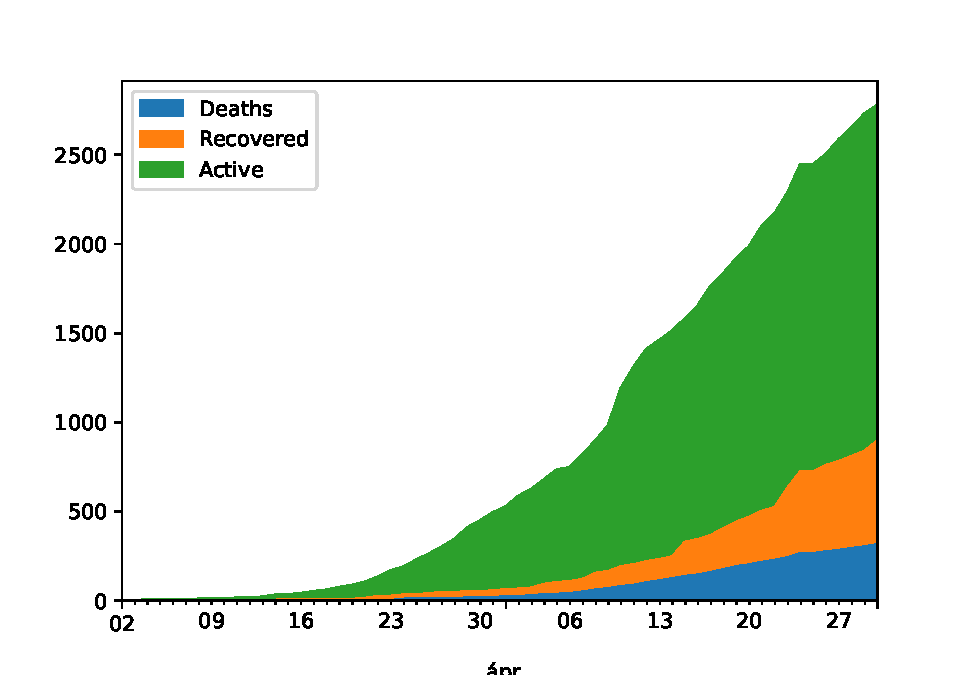
\includegraphics{_main_files/figure-latex/unnamed-chunk-87-1.pdf}

\section{Aggregálás data frame-ben}\label{aggreguxe1luxe1s-data-frame-ben}

Szűrjük le a corona dataframe-ből a legfrissebb adatokat minden országra egy új, corona\_latest dataframe-be!
Maximum függvényünk a \texttt{numpy} csomagból, tehát az \texttt{np} névtérből van.

\begin{Shaded}
\begin{Highlighting}[]
\NormalTok{corona\_latest }\OperatorTok{=}\NormalTok{ corona[corona[}\StringTok{\textquotesingle{}Date\textquotesingle{}}\NormalTok{]}\OperatorTok{==}\NormalTok{np.}\BuiltInTok{max}\NormalTok{(corona[}\StringTok{\textquotesingle{}Date\textquotesingle{}}\NormalTok{])]}
\NormalTok{corona\_latest.info()}
\end{Highlighting}
\end{Shaded}

\begin{verbatim}
## <class 'pandas.core.frame.DataFrame'>
## Index: 264 entries, 26136 to 26399
## Data columns (total 9 columns):
##  #   Column          Non-Null Count  Dtype         
## ---  ------          --------------  -----         
##  0   Province/State  264 non-null    object        
##  1   Country/Region  264 non-null    object        
##  2   Lat             264 non-null    float64       
##  3   Long            264 non-null    float64       
##  4   Date            264 non-null    datetime64[ns]
##  5   Confirmed       264 non-null    int64         
##  6   Deaths          264 non-null    int64         
##  7   Recovered       264 non-null    int64         
##  8   Active          264 non-null    int64         
## dtypes: datetime64[ns](1), float64(2), int64(4), object(2)
## memory usage: 20.6+ KB
\end{verbatim}

Itt mivel egy ország akár lehet több régióval is jelen a sorok között országnév szerint össze tudjuk adni az összes megerősített koronavírusos esetet (\emph{Confirmed} oszlop elemei). Magyarul \textbf{ország szintre szeretnénk összeg segítségével aggregálni} a megerősített koronavírus esetek számát.

Ehhez először a data frame \texttt{groupby} metódusával csoportosítani kell a sorokat ország szintre, majd megadni az összegzendő oszlopot és elsütni ezen oszlop \texttt{sum} metódusát az összegzéshez. Ha a \texttt{sum}-ot \texttt{avg}-re vagy \texttt{median}-ra cseréljük, akkor a kiválasztott oszlopnak nem az összegét, hanem az átlagát, illetve mediánját tudjuk nézni országok szerint. Azaz \textbf{átlaggal/mediánnal is aggregálhatunk az országok szintjére}.

\begin{Shaded}
\begin{Highlighting}[]
\NormalTok{corona\_country }\OperatorTok{=}\NormalTok{ corona\_latest.groupby(}\StringTok{\textquotesingle{}Country/Region\textquotesingle{}}\NormalTok{)[}\StringTok{\textquotesingle{}Confirmed\textquotesingle{}}\NormalTok{].}\BuiltInTok{sum}\NormalTok{()}

\NormalTok{corona\_country.info()}
\end{Highlighting}
\end{Shaded}

\begin{verbatim}
## <class 'pandas.core.series.Series'>
## Index: 187 entries, Afghanistan to Zimbabwe
## Series name: Confirmed
## Non-Null Count  Dtype
## --------------  -----
## 187 non-null    int64
## dtypes: int64(1)
## memory usage: 2.9+ KB
\end{verbatim}

\begin{Shaded}
\begin{Highlighting}[]
\NormalTok{corona\_country.head()}
\end{Highlighting}
\end{Shaded}

\begin{verbatim}
## Country/Region
## Afghanistan    2171
## Albania         773
## Algeria        4006
## Andorra         745
## Angola           27
## Name: Confirmed, dtype: int64
\end{verbatim}

Az eredmény nem egy data frame, hanem mint láthatjuk egy \texttt{Series} lett, ami ugyebár logikailag egy \texttt{numpy} tömb! Mivel a \texttt{groupby} során az országok nevéből lett az új sorindex, így csak 1 oszlopunk maradt, az összegzett megerősített esetszám.

Ha azt szeretnénk, hogy a \textbf{corona\_country}-ben az országok neve ne indexként, hanem külön oszlopként szerepeljen, akkor használjuk a \texttt{reset\_index()} metódust!

\begin{Shaded}
\begin{Highlighting}[]
\NormalTok{corona\_country }\OperatorTok{=}\NormalTok{ corona\_country.reset\_index()}

\NormalTok{corona\_country.info()}
\end{Highlighting}
\end{Shaded}

\begin{verbatim}
## <class 'pandas.core.frame.DataFrame'>
## RangeIndex: 187 entries, 0 to 186
## Data columns (total 2 columns):
##  #   Column          Non-Null Count  Dtype 
## ---  ------          --------------  ----- 
##  0   Country/Region  187 non-null    object
##  1   Confirmed       187 non-null    int64 
## dtypes: int64(1), object(1)
## memory usage: 3.1+ KB
\end{verbatim}

\begin{Shaded}
\begin{Highlighting}[]
\NormalTok{corona\_country.head()}
\end{Highlighting}
\end{Shaded}

\begin{verbatim}
##   Country/Region  Confirmed
## 0    Afghanistan       2171
## 1        Albania        773
## 2        Algeria       4006
## 3        Andorra        745
## 4         Angola         27
\end{verbatim}

Amennyiben a \texttt{groupby} metódus után egy általánosabb \texttt{agg} metódust használunk, akkor a \texttt{groupby}-ban megadott csoportosítás szerint egyszerre több művelet segítségével is összesíthetjük, azaz aggregálhatjuk a számértékű oszlop értékeit (pl. egyszerre nézünk átlagos és medián esetszámokat), Vagy akár több számértékű oszlopot is aggregálhatunk a \texttt{groupby} paraméterei szerint (pl. egyszerre nézünk átlagos esetszámot és halálozást is). Ráadásul, el is tudjuk nevezni az \texttt{agg} függvényen belül az újonnan létrehozott összesítő, azaz aggregált oszlopokat!
Annyi trükk van a dologban, hogy az aggregáláshoz használt függvényeket (medián, átlag, szórás, stb.) a \texttt{numpy} csomagból szedjük ki az \texttt{np.} előtaggal!

Szóval a következő kódrészletben az \texttt{AtlagAktiv\ =\ ("Active",\ np.mean)} rész azt jelenti majd pl, hogy az \emph{AtlagAktiv} oszlop a létrehozandó kimutatástáblában az eredeti data frame \emph{Active} oszlopának átlaggal, azaz \texttt{np.mean} függvényével országos szintre összesített (``\emph{groupby}''-olt) értékeit tartalmazza.

Na, akkor mostmár tényleg készítsünk el egy ország szintű kimutatást az átlagos és medián aktív koronavírus eseteiről, illetve átlagos és medián halálozási számairól a legfrisebb dátumra! Azt is megtehetjük, hogy már az aggregáló kód végére rögtön odatoljuk a \texttt{reset\_index}-et.

\begin{Shaded}
\begin{Highlighting}[]
\NormalTok{corona\_kimutatas }\OperatorTok{=}\NormalTok{ corona\_latest.groupby(}\StringTok{\textquotesingle{}Country/Region\textquotesingle{}}\NormalTok{).agg(}
\NormalTok{  AtlagAktiv }\OperatorTok{=}\NormalTok{ (}\StringTok{"Active"}\NormalTok{, np.mean),}
\NormalTok{  MedianAktiv }\OperatorTok{=}\NormalTok{ (}\StringTok{"Active"}\NormalTok{, np.median),}
\NormalTok{  AtlagHalal }\OperatorTok{=}\NormalTok{ (}\StringTok{"Deaths"}\NormalTok{, np.mean),}
\NormalTok{  MedianHalal }\OperatorTok{=}\NormalTok{ (}\StringTok{"Deaths"}\NormalTok{, np.median)}
\NormalTok{).reset\_index()}
\end{Highlighting}
\end{Shaded}

\begin{verbatim}
## <string>:1: FutureWarning: The provided callable <function mean at 0x00000167D93F13A0> is currently using SeriesGroupBy.mean. In a future version of pandas, the provided callable will be used directly. To keep current behavior pass the string "mean" instead.
## <string>:1: FutureWarning: The provided callable <function median at 0x00000167D95B8720> is currently using SeriesGroupBy.median. In a future version of pandas, the provided callable will be used directly. To keep current behavior pass the string "median" instead.
## <string>:1: FutureWarning: The provided callable <function mean at 0x00000167D93F13A0> is currently using SeriesGroupBy.mean. In a future version of pandas, the provided callable will be used directly. To keep current behavior pass the string "mean" instead.
\end{verbatim}

\begin{Shaded}
\begin{Highlighting}[]
\NormalTok{corona\_kimutatas}
\end{Highlighting}
\end{Shaded}

\begin{verbatim}
##          Country/Region  AtlagAktiv  MedianAktiv  AtlagHalal  MedianHalal
## 0           Afghanistan      1847.0       1847.0        64.0         64.0
## 1               Albania       272.0        272.0        31.0         31.0
## 2               Algeria      1777.0       1777.0       450.0        450.0
## 3               Andorra       235.0        235.0        42.0         42.0
## 4                Angola        18.0         18.0         2.0          2.0
## ..                  ...         ...          ...         ...          ...
## 182  West Bank and Gaza       266.0        266.0         2.0          2.0
## 183      Western Sahara         1.0          1.0         0.0          0.0
## 184               Yemen         4.0          4.0         2.0          2.0
## 185              Zambia        48.0         48.0         3.0          3.0
## 186            Zimbabwe        31.0         31.0         4.0          4.0
## 
## [187 rows x 5 columns]
\end{verbatim}

Azt látjuk, hogy az átlag és medián értékek mind az aktív esetek számára, mind a halálozási számokra megegyeznek. Ez azért van, mert a legtöbb ország ugyebár nem volt lebontva államokra és provinciákra, szóval egy nap csak egy érték érkezett a táblába rájuk mindenből. Egy értéknek pedig nyilván ugyan az az átlaga és a mediánja is! :)

Na, de lessünk meg pár olyan országot, ahol az adatok belső régiókra, provinciákra is le voltak bontva. Pl. Franciaország és az Egyesült Királyság ilyen országok voltak:

\begin{Shaded}
\begin{Highlighting}[]
\NormalTok{corona\_kimutatas[corona\_kimutatas[}\StringTok{"Country/Region"}\NormalTok{].isin([}\StringTok{"France"}\NormalTok{, }\StringTok{"United Kingdom"}\NormalTok{])]}
\end{Highlighting}
\end{Shaded}

\begin{verbatim}
##      Country/Region    AtlagAktiv  MedianAktiv   AtlagHalal  MedianHalal
## 62           France   8409.909091         31.0  2219.090909          1.0
## 177  United Kingdom  13161.818182         13.0  2440.181818          1.0
\end{verbatim}

Na itt már látszik az eltérés! Pl. a francia tartományok felében legfeljebb \(31\) aktív koronavírusos eset volt csak 2020.04.30-án, de a tartományok átlagában az érték már kerektíve \(8410\) eset! Ezt valószínűleg egy vagy kettő kiugróan sok esettel rendlkező tartomány okozza csak!

\section{Egyszerű leíró statisztika data frame-ben}\label{egyszerux171-leuxedruxf3-statisztika-data-frame-ben}

No, de most térjünk vissza a \textbf{corona\_country} data frame-hez! Egyszerűsítsük az oszlopneveket! A data frame-k \texttt{columns} tulajdonságának felülírásával az oszlopnevek könnyen módosíthatók. Mivel ugye a \texttt{columns} tulajdonságban az összes oszlopnév szerepel listaként, így az új oszlopneveket listaként felsorolva {[}{]} jellel kell megadni.

\begin{Shaded}
\begin{Highlighting}[]
\NormalTok{corona\_country.columns}\OperatorTok{=}\NormalTok{[}\StringTok{\textquotesingle{}Country\textquotesingle{}}\NormalTok{, }\StringTok{\textquotesingle{}COVID\_Cases\textquotesingle{}}\NormalTok{]}

\NormalTok{corona\_country.info()}
\end{Highlighting}
\end{Shaded}

\begin{verbatim}
## <class 'pandas.core.frame.DataFrame'>
## RangeIndex: 187 entries, 0 to 186
## Data columns (total 2 columns):
##  #   Column       Non-Null Count  Dtype 
## ---  ------       --------------  ----- 
##  0   Country      187 non-null    object
##  1   COVID_Cases  187 non-null    int64 
## dtypes: int64(1), object(1)
## memory usage: 3.1+ KB
\end{verbatim}

Nézzünk egy komplett leíró statisztikát a \emph{COVID\_Cases} változóra/ismérvre/oszlopra a \texttt{describe} metódus segítségével. Kerekítsük az eredményeket 2 tizedesjegyre (\texttt{round} függvény).

\begin{Shaded}
\begin{Highlighting}[]
\BuiltInTok{round}\NormalTok{(corona\_country.COVID\_Cases.describe(),}\DecValTok{2}\NormalTok{)}
\end{Highlighting}
\end{Shaded}

\begin{verbatim}
## count        187.00
## mean       17416.26
## std        84414.11
## min            1.00
## 25%           97.50
## 50%          746.00
## 75%         6254.50
## max      1069424.00
## Name: COVID_Cases, dtype: float64
\end{verbatim}

Nézzük meg ezt az ordenáré módon jobbra elnyúló eloszlást hisztogramon és doboz ábrán is!

A hisztogramot simán a vizsgált oszlop \texttt{hist} metódusával le lehet kérni.

\begin{Shaded}
\begin{Highlighting}[]
\NormalTok{corona\_country.COVID\_Cases.hist()}
\end{Highlighting}
\end{Shaded}

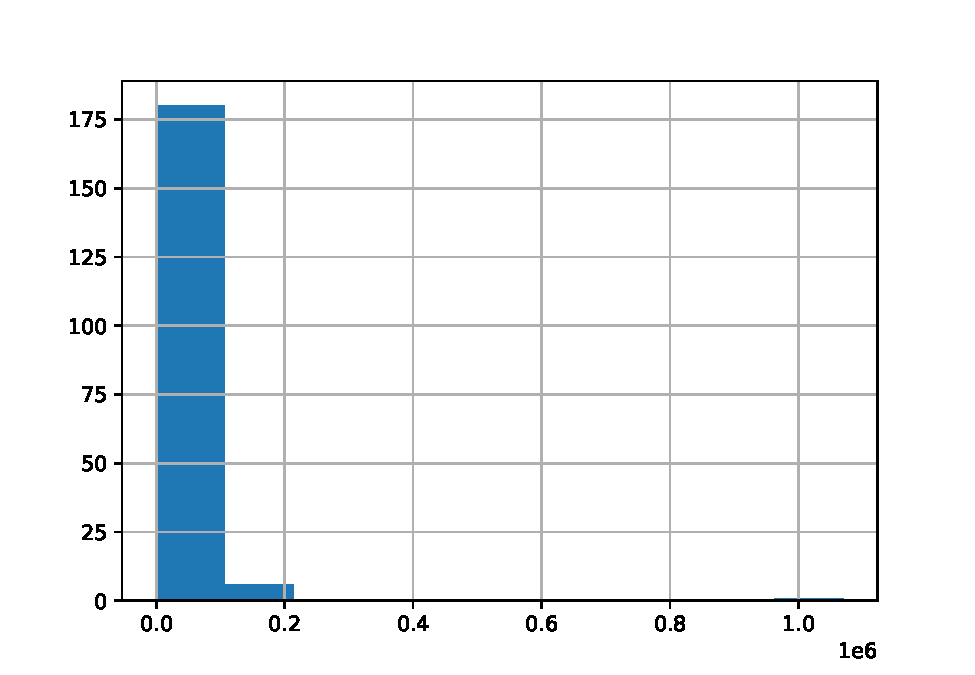
\includegraphics{_main_files/figure-latex/unnamed-chunk-95-3.pdf}

Alapból egyenlő hosszúságú osztályközötket képez a pitonállat a hisztogramokhoz, aminek a számát a \texttt{hist} függvényben a \texttt{bins} paraméteren keresztül tudjuk szabályozni.

Vigyük le pl. az osztályközök számát \(5\)-re.

\begin{Shaded}
\begin{Highlighting}[]
\NormalTok{corona\_country.COVID\_Cases.hist(bins}\OperatorTok{=}\DecValTok{5}\NormalTok{)}
\end{Highlighting}
\end{Shaded}

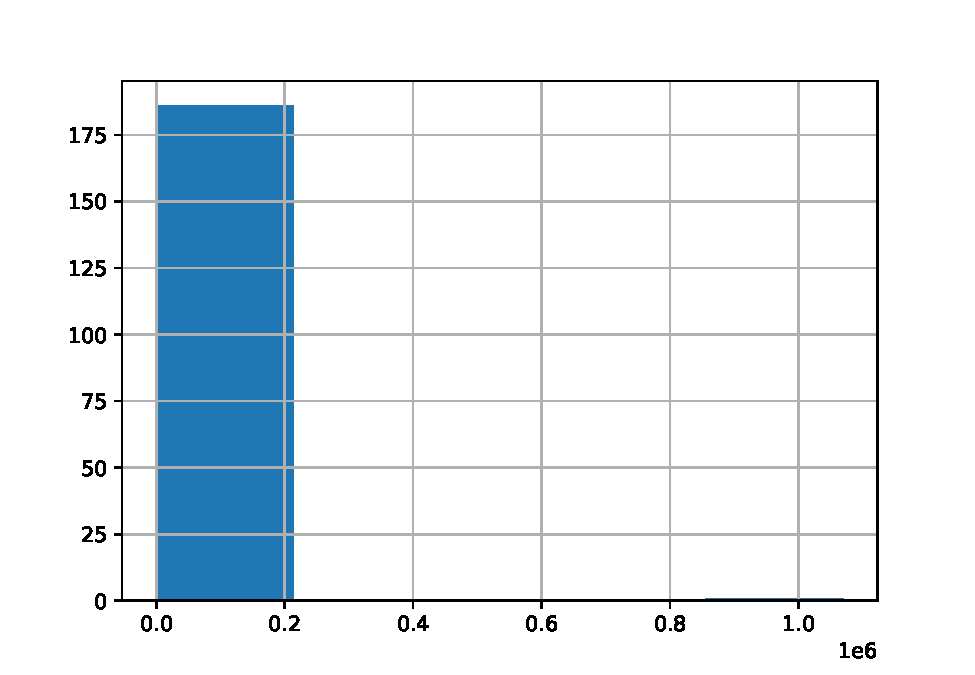
\includegraphics{_main_files/figure-latex/unnamed-chunk-96-5.pdf}

A \texttt{boxplot} metódus már alapvetően data frame, és nem oszlop szinten működik, és a metódus paraméterében kell megadni, hogy mely oszlopra vagy oszlopokra (neveket listaként felsorolva {[}{]} jellel) akarjuk az ábrát. Tehát, a doboz ábrát egyszerre több oszlopra is lekérhetjük egy ábrán belülre akár. Majd mindjárt nézünk ilyet is. Ennek a doboz ábránál van értelme, hiszen doboz ábránál nincsenek osztályközök, amiknek a számát esetlegesen az ismérvünk (oszlopunk) eloszlására kell szabni.

\begin{Shaded}
\begin{Highlighting}[]
\NormalTok{corona\_country.boxplot(column}\OperatorTok{=}\StringTok{"COVID\_Cases"}\NormalTok{)}
\end{Highlighting}
\end{Shaded}

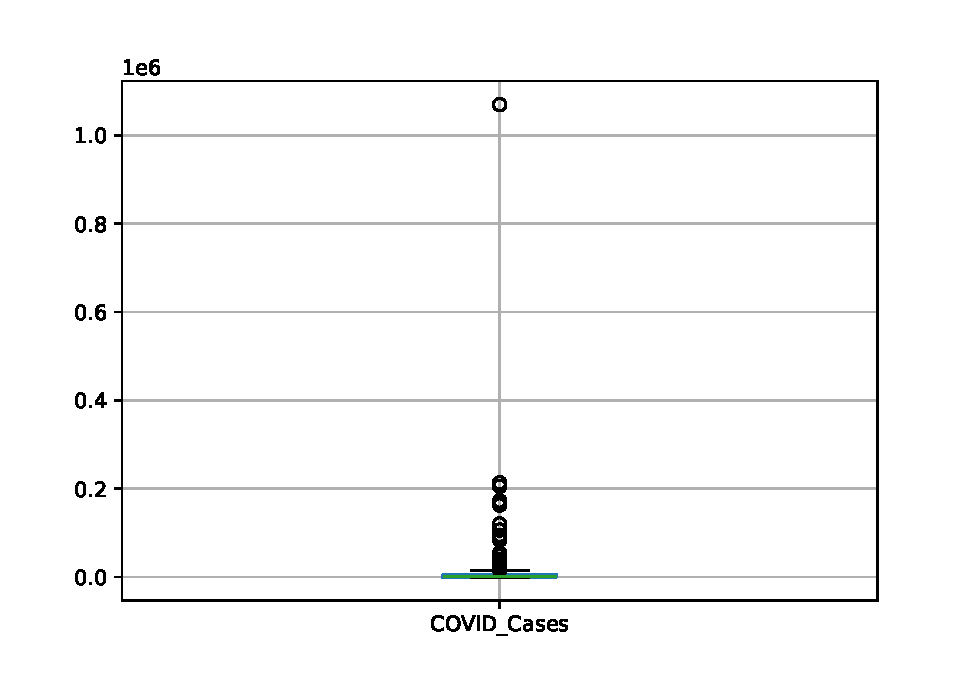
\includegraphics{_main_files/figure-latex/unnamed-chunk-97-7.pdf}

\section{Adatminőségi problémák felismerése és kezelése leíró statisztika segítségével}\label{adatminux151suxe9gi-probluxe9muxe1k-felismeruxe9se-uxe9s-kezeluxe9se-leuxedruxf3-statisztika-seguxedtsuxe9guxe9vel}

Olvassuk be a population\_by\_country\_2020.csv nevű fájlt, és mentsük el a beolvasott adatokat egy \textbf{population} nevű data frame-be!

\begin{Shaded}
\begin{Highlighting}[]
\NormalTok{population }\OperatorTok{=}\NormalTok{ pd.read\_csv(}\StringTok{\textquotesingle{}population\_by\_country\_2020.csv\textquotesingle{}}\NormalTok{)}
\NormalTok{population.info()}
\end{Highlighting}
\end{Shaded}

\begin{verbatim}
## <class 'pandas.core.frame.DataFrame'>
## RangeIndex: 235 entries, 0 to 234
## Data columns (total 11 columns):
##  #   Column                   Non-Null Count  Dtype  
## ---  ------                   --------------  -----  
##  0   Country (or dependency)  235 non-null    object 
##  1   Population (2020)        235 non-null    int64  
##  2   Yearly Change            235 non-null    object 
##  3   Net Change               235 non-null    int64  
##  4   Density (P/Km²)          235 non-null    int64  
##  5   Land Area (Km²)          235 non-null    int64  
##  6   Migrants (net)           201 non-null    float64
##  7   Fert. Rate               235 non-null    object 
##  8   Med. Age                 235 non-null    object 
##  9   Urban Pop %              235 non-null    object 
##  10  World Share              235 non-null    object 
## dtypes: float64(1), int64(4), object(6)
## memory usage: 20.3+ KB
\end{verbatim}

A \textbf{population} dataframe-ből csak az országnév, népesség, népsűrűség és városi népesség aránya változókra lesz szükségünk.
A többit törölhetjük is a data frame-ből! Mivel az oszlopnevekben mint fentebb láthatjuk elég sok a hányadék módon speciális karakter, így biztonságosabb most az oszlopokra a sorszámukkal hivatkozni. Láthatjuk az \texttt{info} metódus eredményéből, hogy a szükséges országnév, népesség, népsűrűség és városi népesség aránya oszlopok rendre a \(0,1,4,9\) indexekkel bírnak.

\begin{Shaded}
\begin{Highlighting}[]
\NormalTok{population }\OperatorTok{=}\NormalTok{ population.iloc[:,[}\DecValTok{0}\NormalTok{, }\DecValTok{1}\NormalTok{, }\DecValTok{4}\NormalTok{, }\DecValTok{9}\NormalTok{]]}

\NormalTok{population.info()}
\end{Highlighting}
\end{Shaded}

\begin{verbatim}
## <class 'pandas.core.frame.DataFrame'>
## RangeIndex: 235 entries, 0 to 234
## Data columns (total 4 columns):
##  #   Column                   Non-Null Count  Dtype 
## ---  ------                   --------------  ----- 
##  0   Country (or dependency)  235 non-null    object
##  1   Population (2020)        235 non-null    int64 
##  2   Density (P/Km²)          235 non-null    int64 
##  3   Urban Pop %              235 non-null    object
## dtypes: int64(2), object(2)
## memory usage: 7.5+ KB
\end{verbatim}

Egyszerűsítsük az oszlopneveket a population dataframe-ben!

\begin{Shaded}
\begin{Highlighting}[]
\NormalTok{population.columns }\OperatorTok{=}\NormalTok{ [}\StringTok{\textquotesingle{}Country\textquotesingle{}}\NormalTok{, }\StringTok{\textquotesingle{}Pop\textquotesingle{}}\NormalTok{, }\StringTok{\textquotesingle{}PopDensity\textquotesingle{}}\NormalTok{, }\StringTok{\textquotesingle{}UrbanPop\textquotesingle{}}\NormalTok{]}

\NormalTok{population.info()}
\end{Highlighting}
\end{Shaded}

\begin{verbatim}
## <class 'pandas.core.frame.DataFrame'>
## RangeIndex: 235 entries, 0 to 234
## Data columns (total 4 columns):
##  #   Column      Non-Null Count  Dtype 
## ---  ------      --------------  ----- 
##  0   Country     235 non-null    object
##  1   Pop         235 non-null    int64 
##  2   PopDensity  235 non-null    int64 
##  3   UrbanPop    235 non-null    object
## dtypes: int64(2), object(2)
## memory usage: 7.5+ KB
\end{verbatim}

Nézzük meg a population dataframe egyszerű leíró statisztikai mutatóit! Ha a \texttt{describe} metódust az egész data frame-n engedjük el, akkor minden numerikus (\texttt{int} vagy \texttt{float}) oszlopra megadja az alap leíró mutatókat.

\begin{Shaded}
\begin{Highlighting}[]
\BuiltInTok{round}\NormalTok{(population.describe(), }\DecValTok{2}\NormalTok{)}
\end{Highlighting}
\end{Shaded}

\begin{verbatim}
##                 Pop  PopDensity
## count  2.350000e+02      235.00
## mean   3.316936e+07      475.77
## std    1.351374e+08     2331.29
## min    8.010000e+02        0.00
## 25%    3.988760e+05       37.00
## 50%    5.459642e+06       95.00
## 75%    2.057705e+07      239.50
## max    1.439324e+09    26337.00
\end{verbatim}

Az \emph{UrbanPop} változónak mi baja? Elviekben az egy arányszám, annak is számnak kéne lennie, és meg kéne jelennie a \texttt{describe} metódus eredményében!

Kukkantsunk csak bele a data frame első 5 sorába!

\begin{Shaded}
\begin{Highlighting}[]
\NormalTok{population.head()}
\end{Highlighting}
\end{Shaded}

\begin{verbatim}
##          Country         Pop  PopDensity UrbanPop
## 0          China  1439323776         153      61%
## 1          India  1380004385         464      35%
## 2  United States   331002651          36      83%
## 3      Indonesia   273523615         151      56%
## 4       Pakistan   220892340         287      35%
\end{verbatim}

Áhhá! Százalékjel van benne! Ezért veszi szöveges adatnak a pitonállat!

Szedjük le ezt a százalékjelet! Erre szerencsére az egyes data frame oszlopoknak van egy \texttt{str.replace} metódusa, amiben megadhatjuk paraméterekkel, hogy az oszlopban milyen szövegrészleteket mire akarunk cserélni. Itt most ugyebár százalékjelet fogunk üres stringre cserélni.

\begin{Shaded}
\begin{Highlighting}[]
\NormalTok{population[}\StringTok{\textquotesingle{}UrbanPop\textquotesingle{}}\NormalTok{] }\OperatorTok{=}\NormalTok{ population[}\StringTok{\textquotesingle{}UrbanPop\textquotesingle{}}\NormalTok{].}\BuiltInTok{str}\NormalTok{.replace(}\StringTok{\textquotesingle{}\%\textquotesingle{}}\NormalTok{, }\StringTok{\textquotesingle{}\textquotesingle{}}\NormalTok{)}

\NormalTok{population.head()}
\end{Highlighting}
\end{Shaded}

\begin{verbatim}
##          Country         Pop  PopDensity UrbanPop
## 0          China  1439323776         153       61
## 1          India  1380004385         464       35
## 2  United States   331002651          36       83
## 3      Indonesia   273523615         151       56
## 4       Pakistan   220892340         287       35
\end{verbatim}

Ez jó, de sajnos vannak benne hiányzó értékek, amik nem a szabványos Python \texttt{NaN} kóddal vannak jelölve, hanem ilyen spéci \emph{``N.A.''} stringgel, amit a gépállat nem ismer fel, így az egész oszlopot \texttt{str}-nek (\texttt{object}) veszi a \texttt{numpy} tömbök egységes adattípus logikája alapján.

\begin{Shaded}
\begin{Highlighting}[]
\NormalTok{population.info()}
\end{Highlighting}
\end{Shaded}

\begin{verbatim}
## <class 'pandas.core.frame.DataFrame'>
## RangeIndex: 235 entries, 0 to 234
## Data columns (total 4 columns):
##  #   Column      Non-Null Count  Dtype 
## ---  ------      --------------  ----- 
##  0   Country     235 non-null    object
##  1   Pop         235 non-null    int64 
##  2   PopDensity  235 non-null    int64 
##  3   UrbanPop    235 non-null    object
## dtypes: int64(2), object(2)
## memory usage: 7.5+ KB
\end{verbatim}

Azt, hogy az \texttt{object} adattípus turpisságát az ``N.A.''-k okozzák az UrbanPop oszlopban, arra leginkább az oszlop gyakorisági táblájából lehet felismerni. Ezt a gyakorisági táblát az oszlop \texttt{value\_counts} metódusával tudjuk lekérni.

\begin{Shaded}
\begin{Highlighting}[]
\NormalTok{population.UrbanPop.value\_counts()}
\end{Highlighting}
\end{Shaded}

\begin{verbatim}
## UrbanPop
## N.A.    13
## 57       7
## 88       7
## 63       6
## 87       6
##         ..
## 50       1
## 81       1
## 28       1
## 37       1
## 10       1
## Name: count, Length: 81, dtype: int64
\end{verbatim}

Láthatjuk, hogy a sok számérték mellett, 13 ország esetén hiányzó értékünk van ezzel a csúnya ``N.A.'' kóddal.

Na, akkor! Most csináljuk azt, hogy leszűrjük azt a 13 országot, ahol hiányzik a városi népesség arányára vonatkozó adat!

Ezek után próbáljuk meg a városi népesség arányára vonatkozó adatot \texttt{int} típusúvá konvertálni! Ha sikerült, nézzük meg a változó alap leíró statisztikai mutatóit is!

Először logikai indexszeléssel leszűrjük az ``N.A.''-kat.

\begin{Shaded}
\begin{Highlighting}[]
\NormalTok{population }\OperatorTok{=}\NormalTok{ population[population[}\StringTok{\textquotesingle{}UrbanPop\textquotesingle{}}\NormalTok{]}\OperatorTok{!=}\StringTok{"N.A."}\NormalTok{]}
\end{Highlighting}
\end{Shaded}

Majd az oszlop \texttt{astype} metódusával \texttt{int}-é konvertáljuk az egész oszlopot. A metódus paraméterében kell megadni, hogy milyen adattípusra akarjuk konvertálni kiszemelt kis oszlopunk! :) Végül jöhet a \texttt{describe}.

\begin{Shaded}
\begin{Highlighting}[]
\NormalTok{population[}\StringTok{\textquotesingle{}UrbanPop\textquotesingle{}}\NormalTok{] }\OperatorTok{=}\NormalTok{ population[}\StringTok{\textquotesingle{}UrbanPop\textquotesingle{}}\NormalTok{].astype(}\BuiltInTok{int}\NormalTok{)}

\NormalTok{population.describe()}
\end{Highlighting}
\end{Shaded}

\begin{verbatim}
##                 Pop   PopDensity    UrbanPop
## count  2.220000e+02   222.000000  222.000000
## mean   3.488611e+07   186.373874   59.234234
## std    1.388508e+08   288.271695   24.230400
## min    1.357000e+03     0.000000    0.000000
## 25%    5.444048e+05    35.000000   43.000000
## 50%    5.911701e+06    89.000000   60.500000
## 75%    2.321589e+07   224.500000   79.000000
## max    1.439324e+09  2239.000000  100.000000
\end{verbatim}

Úgy tűnik, helyreállt a világ rendje! Már nagyon szépen le tudjuk olvasni pl., hogy a Föld országainak legzsúfoltabb \(25\%\)-ban legalább \(79\) fő/Km² a népsűrűség. És azt is látni a \texttt{count}ból, hogy már csak \(222\) országunk van a kezdeti \(235\) helyett, szóval nincsen itt a \(13\) ``N.A.''.

\section{Data frame-k összekapcsolása}\label{data-frame-k-uxf6sszekapcsoluxe1sa}

Akkor most álmodjunk egy nagyot! Kössük össze a \textbf{population} data frame-ben található országonkénti alapvető demográfiai ismérveket a \textbf{corona\_country} data frame-ben lakó országonkénti koronavírus esetszámokkal.

Nyilván ezt az összekötést az országok nevén keresztül lehet megtenni. Azaz pl. a magyar koronavírus esetszámokhoz a magyar demográfiai adatoknak kell kerülnie értelemszerűen. :)

A \texttt{pandas} csomagnak létezik egy \texttt{merge} névre hallgató függvénye, ami két data frame-et összeköt egy előre megadott közös oszlop alapján. Esetünkben ez a közös oszlop az országnév lesz.
Ha egy kicsit ``\emph{adatbázisabbul}'' szeretném kifejezni magam, akkor azt mondanám, hogy a \texttt{merge} függvény 2 tábla joinját oldja meg egy közös kulcs alapján.

Sőt, a \texttt{merge} függvény mindhárom alapvető táblakapcsolási módszert támogatja:

\begin{itemize}
\tightlist
\item
  \textbf{inner join}: Az összekötött táblában csak azok a sorok maradnak meg, amelyek mindkét data frame-ben szerepelnek.
\item
  \textbf{left join}: Az összekötött táblában csak azok a sorok maradnak meg, amelyek az elsőre megnevezett data frame-ben szerepelnek (attól függetlenül, hogy a másodszorra megnevezett táblában van-e hozzájuk találat).
\item
  \textbf{right join}: Az összekötött táblában csak azok a sorok maradnak meg, amelyek a másodszorra megnevezett data frame-ben szerepelnek (attól függetlenül, hogy az elsőre megnevezett táblában van-e hozzájuk találat).
\item
  \textbf{full outer join}: Az összekötött táblában mindkét tábla minden sora megmarad.
\end{itemize}

A különböző típusú összekötési módokat remekül lehet halmazábrákkal szemléltetni:

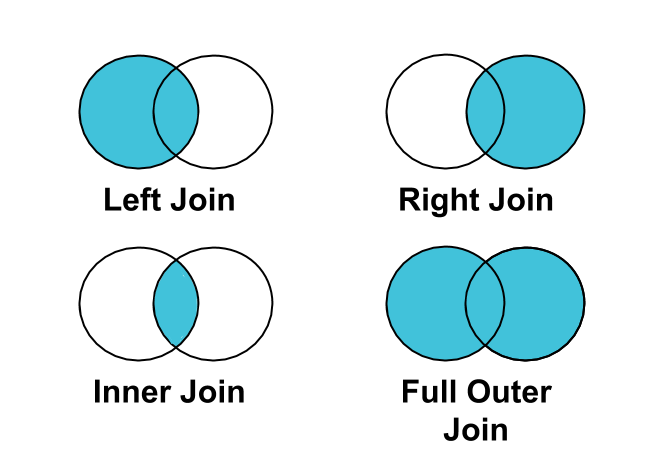
\includegraphics[width=0.5\textwidth,height=\textheight]{JoinVennDiagram.png}

Na, akkor mielőtt a tényleges \texttt{merge}-hez hozzálátunk, annyit ellenőrizzünk le, hogy ugyanaz-e a neve az országneveket tartalmazó oszlopnak mindkét data frame-ben, a \textbf{population}ben és a \textbf{corona\_country}-ban is:

\begin{Shaded}
\begin{Highlighting}[]
\NormalTok{corona\_country.columns}
\end{Highlighting}
\end{Shaded}

\begin{verbatim}
## Index(['Country', 'COVID_Cases'], dtype='object')
\end{verbatim}

\begin{Shaded}
\begin{Highlighting}[]
\NormalTok{population.columns}
\end{Highlighting}
\end{Shaded}

\begin{verbatim}
## Index(['Country', 'Pop', 'PopDensity', 'UrbanPop'], dtype='object')
\end{verbatim}

Szuper, mindkét táblában egységesen \textbf{`Country'} az összekötésre használandó oszlop neve! Nem meglepő, mert mindkét táblában átneveztük már korábban az oszlopokat, de azért jobb biztosra menni. :)

Akkor lássuk azt a \texttt{merge}-t! Most egy olyan összekötést csinálunk, hogy a \textbf{corona\_country} táblában lévő összes sorunk maradjon meg az összekötött táblában, mert alapvetően azok az országok érdekelnek, ahol megvan a COVID fertőzöttek száma. Ez az én data frame megadási sorrendben majd egy \emph{left join}t fog jelenteni. :)

A \texttt{merge} függvényben a két data frame megadása után a \texttt{how} paraméter szabályozza a \emph{join} jellegét, míg az \texttt{on} paraméterben adjuk meg az összekötésre használt oszlop nevét. A \emph{join} tehát azért lesz \emph{left}, mert a \textbf{corona\_country}-t adtam meg először, azaz ``\emph{balrább}''. :)

\begin{Shaded}
\begin{Highlighting}[]
\NormalTok{corona\_extended }\OperatorTok{=}\NormalTok{ pd.merge(corona\_country, population, how}\OperatorTok{=}\StringTok{\textquotesingle{}left\textquotesingle{}}\NormalTok{, on}\OperatorTok{=}\StringTok{\textquotesingle{}Country\textquotesingle{}}\NormalTok{)}
\NormalTok{corona\_extended.info()}
\end{Highlighting}
\end{Shaded}

\begin{verbatim}
## <class 'pandas.core.frame.DataFrame'>
## RangeIndex: 187 entries, 0 to 186
## Data columns (total 5 columns):
##  #   Column       Non-Null Count  Dtype  
## ---  ------       --------------  -----  
##  0   Country      187 non-null    object 
##  1   COVID_Cases  187 non-null    int64  
##  2   Pop          168 non-null    float64
##  3   PopDensity   168 non-null    float64
##  4   UrbanPop     168 non-null    float64
## dtypes: float64(3), int64(1), object(1)
## memory usage: 7.4+ KB
\end{verbatim}

Na, hát az új data frame \texttt{info} metódusa alapján van egy kis probléma. \(187-168=19\) országra a \textbf{corona\_country} data frame-ben nem volt találat a \textbf{population} data frame-ben.

\subsection{A kapcsolási kulcsnak használt oszlop ellenőrzése és javítása}\label{a-kapcsoluxe1si-kulcsnak-hasznuxe1lt-oszlop-ellenux151rzuxe9se-uxe9s-javuxedtuxe1sa}

Lessük meg mik ezek az országok, ahol nem volt találat a \textbf{population} data frame-ben! Ezt pl. úgy tudjuk megtenni, hogy lekérdezzük a hiányzó értékek országát a \textbf{Pop} oszlopban.

\begin{Shaded}
\begin{Highlighting}[]
\NormalTok{corona\_extended.Country[corona\_extended.Pop.isnull()}\OperatorTok{==}\VariableTok{True}\NormalTok{]}
\end{Highlighting}
\end{Shaded}

\begin{verbatim}
## 27                                Burma
## 39                  Congo (Brazzaville)
## 40                     Congo (Kinshasa)
## 42                        Cote d'Ivoire
## 46                              Czechia
## 48                     Diamond Princess
## 75                             Holy See
## 91                               Kosovo
## 92                               Kuwait
## 102                          MS Zaandam
## 113                              Monaco
## 140               Saint Kitts and Nevis
## 142    Saint Vincent and the Grenadines
## 144               Sao Tome and Principe
## 150                           Singapore
## 164                             Taiwan*
## 173                                  US
## 180                           Venezuela
## 182                  West Bank and Gaza
## Name: Country, dtype: object
\end{verbatim}

Elnézegetve az országneveket kialakulhat bennünk valami sejtés: valószínűleg ezeket az országokat máshogy hívják a \textbf{population} data frame-ben, mint a \textbf{corona\_country}-ban. Pl. \emph{Taiwan} nevében valószínűleg nem lesz csillag, vagy \emph{Czechia}-t inkább a hivatalosabb nevén jegyezheti a \textbf{population} tábla: \emph{Czech Republic}. Esetleg a \emph{US} is inkább \emph{United States}-ként szerepelhet.

Teszteljük le ezeket az elméleteket egy egyszerű logikai indexes szűréssel az \texttt{isin} metódussal megtámogatva.

\begin{Shaded}
\begin{Highlighting}[]
\NormalTok{population.Country[population.Country.isin([}\StringTok{"Czech Republic"}\NormalTok{, }\StringTok{"Taiwan"}\NormalTok{, }\StringTok{"United States"}\NormalTok{])]}
\end{Highlighting}
\end{Shaded}

\begin{verbatim}
## 2     United States
## 56           Taiwan
## Name: Country, dtype: object
\end{verbatim}

Mintha bejönne az okoskodásunk, de a cseheket csak nem akarja megtalálni a cucc. Próbáljunk meg úgy szűrni, hogy ne pontosan keressük ezeket az országneveket, hanem azt nézzük meg, hogy mik azok a sorok a \textbf{population} data frame-ben, amik ezeket az országneveket \emph{tartalmazzák} valahol a \textbf{Country} oszlopban.
Ezt egyszerűen el tudjuk érni úgy, hogy az előző kódunkban az \texttt{isin} metódust \texttt{str.contains}-re cseréljük. Annyi van, hogy itt a keresett string mintázatokat egy stringben kell megadni (azaz NEM listaként) ``\textbar{}'' jellel elválasztva őket.
Ez így amúgy egy úgynevezett \href{http://vbence.web.elte.hu/regex_leiras.html}{RegEx kifejezés}, és ilyenekkel lehet komplexebben működtetni ezt a \texttt{str.contains} metódust. Az érdeklődőknek jó kiindulópont a link. :)

\begin{Shaded}
\begin{Highlighting}[]
\NormalTok{population.Country[population.Country.}\BuiltInTok{str}\NormalTok{.contains(}\StringTok{"Czech Republic|Taiwan|United States"}\NormalTok{)]}
\end{Highlighting}
\end{Shaded}

\begin{verbatim}
## 2                United States
## 56                      Taiwan
## 85    Czech Republic (Czechia)
## Name: Country, dtype: object
\end{verbatim}

Ó, hogy a kedves felmenőiket a \textbf{population} data frame alkotóinak: hát nem ott van zárójelben a \emph{Czech Republic} mögött, hogy \emph{Czechia}?! ``\emph{Ripsz!}''

Hát valami hasonló módon be kéne lőni a maradék 16 nem egyező országnevet is, de most ezzel nem húzzuk a drága időnket, hanem javítjuk ezt a 3 esetet és újra összekötjük a tábláinkat.
Aki a nem egyértelmű kapcsoló oszlop (kulcs) alapján történő data frame összekötés világában szeretne elmélyedni, neki érdemes lehet majd előbb-utóbb utána néznie a \emph{fuzzy join} technikáknak, amiket a Pythonban pl. a \href{https://stackoverflow.com/questions/13636848/is-it-possible-to-do-fuzzy-match-merge-with-python-pandas}{difflib csomag támogat}. De ezek a megoldások az itteni bevezető példának a kereteit bőven megugorják komplexitásban.

Szóval, akkor a 3 azonosított eltérő országnevet javítsuk a \textbf{population} data frame-ben. Azaz ott átírjuk ezeket az országneveket arra a verzióra, ami a \textbf{corona\_country}-ban is szerepel. Ehhez megint az \texttt{str.replace}-t használjuk, mint anno az \textbf{UrbanPop} oszlop százalékjeleinek eltávolításakor. Ezt mindhárom esetben külön meg kell sajnos tenni.

\begin{Shaded}
\begin{Highlighting}[]
\NormalTok{population[}\StringTok{\textquotesingle{}Country\textquotesingle{}}\NormalTok{] }\OperatorTok{=}\NormalTok{ population[}\StringTok{\textquotesingle{}Country\textquotesingle{}}\NormalTok{].replace(}\StringTok{\textquotesingle{}United States\textquotesingle{}}\NormalTok{, }\StringTok{\textquotesingle{}US\textquotesingle{}}\NormalTok{)}
\NormalTok{population[}\StringTok{\textquotesingle{}Country\textquotesingle{}}\NormalTok{] }\OperatorTok{=}\NormalTok{ population[}\StringTok{\textquotesingle{}Country\textquotesingle{}}\NormalTok{].replace(}\StringTok{\textquotesingle{}Czech Republic (Czechia)\textquotesingle{}}\NormalTok{, }\StringTok{\textquotesingle{}Czechia\textquotesingle{}}\NormalTok{)}
\NormalTok{population[}\StringTok{\textquotesingle{}Country\textquotesingle{}}\NormalTok{] }\OperatorTok{=}\NormalTok{ population[}\StringTok{\textquotesingle{}Country\textquotesingle{}}\NormalTok{].replace(}\StringTok{\textquotesingle{}Taiwan\textquotesingle{}}\NormalTok{, }\StringTok{\textquotesingle{}Taiwan*\textquotesingle{}}\NormalTok{)}
\end{Highlighting}
\end{Shaded}

És akkor lássuk újra azt a \texttt{merge}-t! Most a többi nem kezelt esetet eldobjuk, szóval \emph{inner join}t csinálunk.

\begin{Shaded}
\begin{Highlighting}[]
\NormalTok{corona\_extended }\OperatorTok{=}\NormalTok{ pd.merge(corona\_country, population, how}\OperatorTok{=}\StringTok{\textquotesingle{}inner\textquotesingle{}}\NormalTok{, on}\OperatorTok{=}\StringTok{\textquotesingle{}Country\textquotesingle{}}\NormalTok{)}
\NormalTok{corona\_extended.info()}
\end{Highlighting}
\end{Shaded}

\begin{verbatim}
## <class 'pandas.core.frame.DataFrame'>
## RangeIndex: 171 entries, 0 to 170
## Data columns (total 5 columns):
##  #   Column       Non-Null Count  Dtype 
## ---  ------       --------------  ----- 
##  0   Country      171 non-null    object
##  1   COVID_Cases  171 non-null    int64 
##  2   Pop          171 non-null    int64 
##  3   PopDensity   171 non-null    int64 
##  4   UrbanPop     171 non-null    int32 
## dtypes: int32(1), int64(3), object(1)
## memory usage: 6.1+ KB
\end{verbatim}

Szupszi! Már nem \(168\) sor van, amire van találat mindkét data frame-ben, mint az előbb, hanem \(171\), azaz pont a megjavított \(3\) országgal több! Na, erre már elő lehet venni az ünnepi laposüveget (leánykori nevén lapiüvit)! ;)

\section{Kilógó értékek keresése és kezelése}\label{kiluxf3guxf3-uxe9rtuxe9kek-keresuxe9se-uxe9s-kezeluxe9se}

A sikeres data frame összekötési művelet örömére, számoljuk ki a \textbf{corona\_extended} dataframe-ben az egymillió főre jutó COVID-19 esetek számát minden országra! Aztán nézzük is meg az oszlop leíró statisztikáit!

\begin{Shaded}
\begin{Highlighting}[]
\NormalTok{corona\_extended[}\StringTok{\textquotesingle{}COVID\_perMillion\textquotesingle{}}\NormalTok{] }\OperatorTok{=}\NormalTok{ corona\_extended.COVID\_Cases }\OperatorTok{/}\NormalTok{ corona\_extended.Pop }\OperatorTok{*} \DecValTok{1000000}
\NormalTok{corona\_extended[}\StringTok{\textquotesingle{}COVID\_perMillion\textquotesingle{}}\NormalTok{].describe()}
\end{Highlighting}
\end{Shaded}

\begin{verbatim}
## count      171.000000
## mean       747.439425
## std       1775.534029
## min          0.201167
## 25%         19.420289
## 50%        119.830206
## 75%        700.197689
## max      16769.325985
## Name: COVID_perMillion, dtype: float64
\end{verbatim}

Na, szuper, itt is látszik egy csodás jobbra elnyúló eloszlás, hiszen az országok \(\frac{3}{4}\)-ének az egymillió főre vetített COVID esetszáma nem haladja meg a \(700\)-at, de ellenben a legnagyobb érték már majdnem \(17\) ezer fő! Ellenben az alsó \(25\%\) határa, a \(19.4\) egészen közel van a minimumhoz, a \(0.2\)-höz. Szóval valószínűleg brutál felfelé kilógó elemeink vannak.

Ezt erősítsük is meg egy doboz ábrán.

\begin{Shaded}
\begin{Highlighting}[]
\NormalTok{corona\_extended.boxplot(column}\OperatorTok{=}\StringTok{"COVID\_perMillion"}\NormalTok{)}
\end{Highlighting}
\end{Shaded}

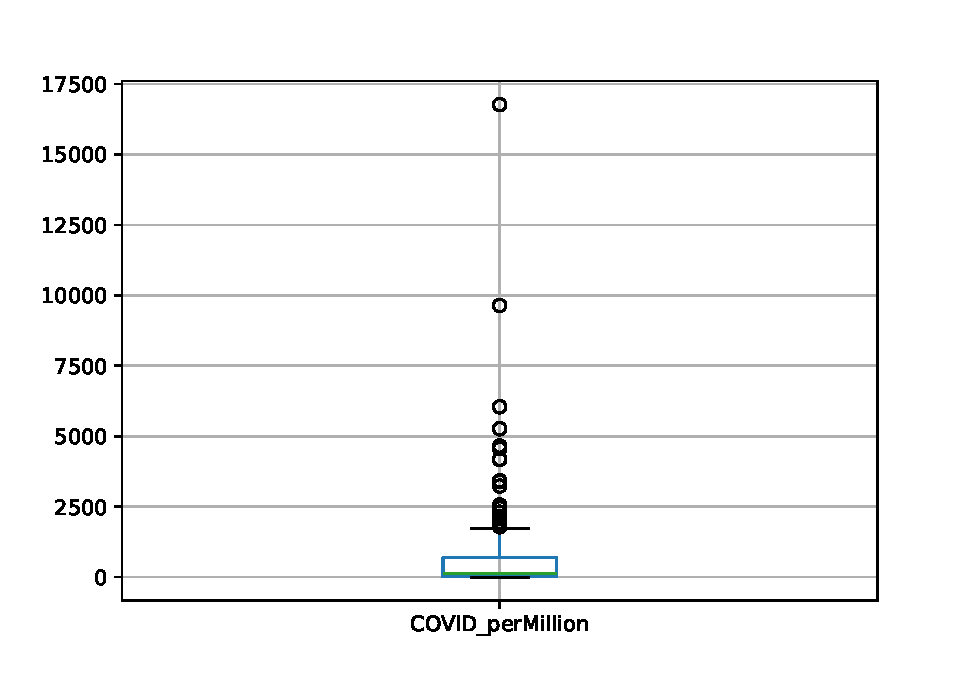
\includegraphics{_main_files/figure-latex/unnamed-chunk-116-9.pdf}

Az ábra alapján nagyjából olyan 3000 feletti értékek tűnnek extrém módon kilógónak (kb. 3000-nél van az első szakadás a dobozban a ponttal jelölt kilógó értékek körében; a szakadás alatti részek, még kb a normál adatok ``természetes'' folytatásának tekinthetők). Lássuk hát, hogy mik ezek!

Rendezzük a \textbf{COVID\_perMillion} szerint csökkenő sorrendbe a data frame-t, és kérjük le a sorbarendezett verzióból azokat az értékeket, ahol a \textbf{COVID\_perMillion} nagyobb, mint 3000!

A data frame-t sorba rendezni a \texttt{sort\_values} metódussal lehet, amelynek paraméterében meg kell adni, hogy mely oszlop alapján rendezünk, és hogy a sorrend csökkenő vagy növekvő-e. Majd ezen a rendezett állapoton elsüthetünk pl. egy iloc-ot az első 10 sor kiválasztásához.

\begin{Shaded}
\begin{Highlighting}[]
\NormalTok{corona\_extended.sort\_values(}\StringTok{\textquotesingle{}COVID\_perMillion\textquotesingle{}}\NormalTok{, ascending}\OperatorTok{=}\VariableTok{False}\NormalTok{).loc[corona\_extended[}\StringTok{\textquotesingle{}COVID\_perMillion\textquotesingle{}}\NormalTok{] }\OperatorTok{\textgreater{}} \DecValTok{3000}\NormalTok{,:]}
\end{Highlighting}
\end{Shaded}

\begin{verbatim}
##          Country  COVID_Cases  ...  UrbanPop  COVID_perMillion
## 131   San Marino          569  ...        97      16769.325985
## 3        Andorra          745  ...        88       9642.140685
## 93    Luxembourg         3784  ...        88       6044.940877
## 72       Iceland         1797  ...        94       5266.042087
## 126        Qatar        13409  ...        96       4654.201086
## 143        Spain       213435  ...        80       4564.987989
## 16       Belgium        48519  ...        98       4186.417453
## 77       Ireland        20612  ...        63       4174.340484
## 148  Switzerland        29586  ...        74       3418.520185
## 79         Italy       205463  ...        69       3398.226842
## 159           US      1069424  ...        83       3230.862341
## 
## [11 rows x 6 columns]
\end{verbatim}

Na, úgy néz ki, hogy az érintett országok töbségében ilyen jó kicsi, zsúfolt államok. Persze vannak extrém kivételek, pl. ugye az olaszok a nagy repülős turistaforgalmuk miatt.

Na, ezeket az extrém módon kilógó értékeket kipucoljuk a data frame-ből, aztán ránézünk újra a \textbf{COVID\_perMillion} doboz ábrájára. Most a kilógó értékeket vegyük csak a 4000 feletti esetszámoknak, mivel a sorrend alapján van egy nagyobb ugrás ott a svájci 3418-ról az ír 4174-re. Meg a doboz ábrán is látszik, hogy ez az utolsó 3 érték ebben a ``toplistában'' még azért közelebb van az adatok ``természetes folytatásához'', és utána jön még egy ugrás az egymillió főre vetített esetszámokban.

\begin{Shaded}
\begin{Highlighting}[]
\NormalTok{corona\_extended }\OperatorTok{=}\NormalTok{ corona\_extended[corona\_extended[}\StringTok{\textquotesingle{}COVID\_perMillion\textquotesingle{}}\NormalTok{] }\OperatorTok{\textless{}} \DecValTok{4000}\NormalTok{]}
\NormalTok{corona\_extended.boxplot(column}\OperatorTok{=}\StringTok{"COVID\_perMillion"}\NormalTok{)}
\end{Highlighting}
\end{Shaded}

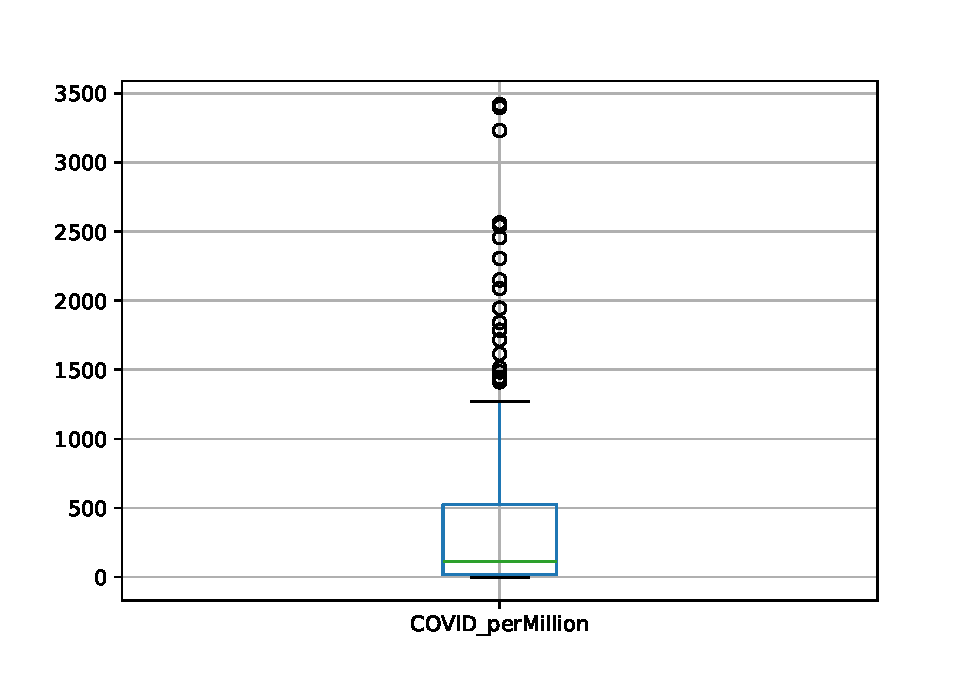
\includegraphics{_main_files/figure-latex/unnamed-chunk-118-11.pdf}

Ez már egy kulturáltabb jobbra elnyúló eloszlás. Viszont, a medián még mindig túlságosan közel van az alsó kvartilishez, és a felső kvartilis eléggé elszakad.

Ennek szellemében még nézzünk rá arra, hogy mely országok esnek az egymillió főre jutó COVID esetszám szerint az alsó kvintilisbe!

Egy data frame oszlop alsó kvintilisét az oszlop \texttt{quantile} metódusával számoljuk ki. A metódus alapvetően egy tetszőleges percentilist számol ki. Azt, hogy melyiket, azt a metódus paraméterében kell megadni \(0-1\) közötti számként. Szóval az alsó kvintilis alias 20. percentilis, ami alatt az adatok \(20\%\)-a található, egy \(0.2\) paraméterrel lesz megadható.

\begin{Shaded}
\begin{Highlighting}[]
\NormalTok{corona\_extended[}\StringTok{\textquotesingle{}COVID\_perMillion\textquotesingle{}}\NormalTok{].quantile(}\FloatTok{0.2}\NormalTok{)}
\end{Highlighting}
\end{Shaded}

\begin{verbatim}
## 10.058723607815136
\end{verbatim}

Ezt a fenti kódot felhasználva egy logikai indexes szűrésben gyorsan meg is lesznek a népességarányos esetszám szerinti alsó kvintilisbe tartozó országok nevei is.

\begin{Shaded}
\begin{Highlighting}[]
\NormalTok{corona\_extended[corona\_extended[}\StringTok{\textquotesingle{}COVID\_perMillion\textquotesingle{}}\NormalTok{] }\OperatorTok{\textless{}} 
\NormalTok{               corona\_extended[}\StringTok{\textquotesingle{}COVID\_perMillion\textquotesingle{}}\NormalTok{].quantile(}\FloatTok{0.2}\NormalTok{)]}
\end{Highlighting}
\end{Shaded}

\begin{verbatim}
##               Country  COVID_Cases  ...  UrbanPop  COVID_perMillion
## 4              Angola           27  ...        67          0.821511
## 18              Benin           64  ...        48          5.279134
## 19             Bhutan            7  ...        46          9.071964
## 22           Botswana           23  ...        73          9.780463
## 27            Burundi           11  ...        14          0.925086
## 29           Cambodia          122  ...        24          7.297102
## 33               Chad           73  ...        23          4.444211
## 37            Comoros            1  ...        29          1.149953
## 54           Ethiopia          131  ...        21          1.139491
## 59             Gambia           11  ...        59          4.551722
## 69              Haiti           81  ...        57          7.103688
## 84              Kenya          396  ...        28          7.364524
## 86               Laos           19  ...        36          2.611483
## 90              Libya           61  ...        78          8.877515
## 94         Madagascar          128  ...        39          4.622437
## 95             Malawi           37  ...        18          1.934140
## 100        Mauritania            8  ...        57          1.720557
## 107        Mozambique           76  ...        38          2.431577
## 108           Namibia           16  ...        55          6.296969
## 109             Nepal           57  ...        21          1.956288
## 112         Nicaragua           14  ...        57          2.113350
## 114           Nigeria         1932  ...        52          9.372290
## 120  Papua New Guinea            8  ...        13          0.894152
## 142       South Sudan           35  ...        25          3.126752
## 149             Syria           43  ...        60          2.457050
## 151        Tajikistan           15  ...        27          1.572715
## 152          Tanzania          480  ...        37          8.035595
## 160            Uganda           83  ...        26          1.814564
## 166           Vietnam          270  ...        38          2.773823
## 167    Western Sahara            6  ...        87         10.044548
## 168             Yemen            6  ...        38          0.201167
## 169            Zambia          106  ...        45          5.765897
## 170          Zimbabwe           40  ...        38          2.691260
## 
## [33 rows x 6 columns]
\end{verbatim}

Az eredmények alapján úgy néz ki, hogy az egymillió főre jutó COVID esetszám szerinti alsó kvintilisbe elsősorban olyan afrikai országok esnek, ahol még 2020.04.30-án egyelőre nem tört ki tömeges járvány!

Ezeket az országokat távolítsuk el a corona\_country dataframe-ből!
Majd ezután tekintsük meg ismét az egymillió főre jutó COVID esetszám hisztogramját, és doboz ábráját!

\begin{Shaded}
\begin{Highlighting}[]
\NormalTok{corona\_extended }\OperatorTok{=}\NormalTok{ corona\_extended[corona\_extended[}\StringTok{\textquotesingle{}COVID\_perMillion\textquotesingle{}}\NormalTok{] }\OperatorTok{\textgreater{}}
\NormalTok{                                corona\_extended[}\StringTok{\textquotesingle{}COVID\_perMillion\textquotesingle{}}\NormalTok{].quantile(}\FloatTok{.2}\NormalTok{)]}

\NormalTok{corona\_extended.boxplot(column}\OperatorTok{=}\StringTok{"COVID\_perMillion"}\NormalTok{)}
\end{Highlighting}
\end{Shaded}

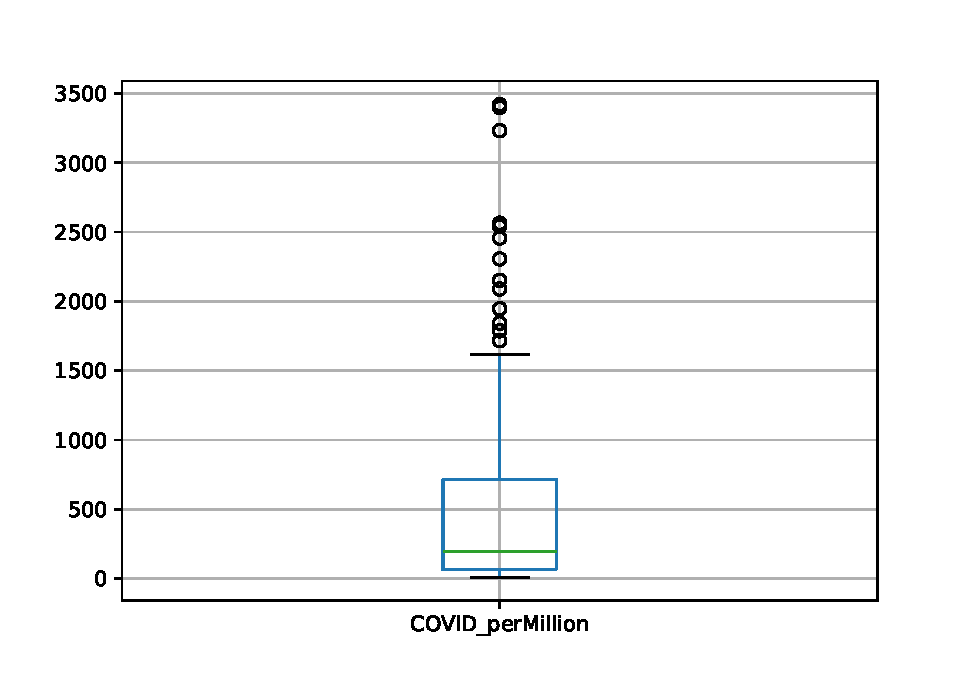
\includegraphics{_main_files/figure-latex/unnamed-chunk-121-13.pdf}

Na, ez már kb úgy néz ki, mint egy ``egészségesen'' jobbra elnyúló eloszlás doboz ábrája! :)

\section{Korrelációs elemzések data frame-ben}\label{korreluxe1ciuxf3s-elemzuxe9sek-data-frame-ben}

Nézzünk rá a numerikus adattípusú oszlopok közti korrelációs mátrixra. Egyedül a \textbf{Pop} és \textbf{COVID\_Cases} oszlopokat hagyjuk ki a vizsgálatból, mert azok abszolút és nem népességarányos adatok, így csalóka lenne őket szerepeltetni a korrelációs vizsgálatokban, hiszen ``triviálisan'' korrelálnak: nagyobb népességű országban nyilván több az összes esetszám. :)

Azt, hogy csak két oszlopot ne válasszunk ki egy data frame-ben úgy tudjuk elérni, hogy a data frame oszlopnevei közül egy \texttt{isin} metódussal kiválasztjuk a két kihagyandó oszlopot, majd az eredményt letagadjuk egy \texttt{\textasciitilde{}} jellel. Ezt a műveletet pedig beágyazzuk egy \texttt{loc} metódusba, és meg is vagyunk! :)

\begin{Shaded}
\begin{Highlighting}[]
\NormalTok{corona\_extended.loc[:,}\OperatorTok{\textasciitilde{}}\NormalTok{corona\_extended.columns.isin([}\StringTok{\textquotesingle{}COVID\_Cases\textquotesingle{}}\NormalTok{, }\StringTok{\textquotesingle{}Pop\textquotesingle{}}\NormalTok{])]}
\end{Highlighting}
\end{Shaded}

\begin{verbatim}
##                   Country  PopDensity  UrbanPop  COVID_perMillion
## 0             Afghanistan          60        25         55.769130
## 1                 Albania         105        63        268.608244
## 2                 Algeria          18        73         91.354724
## 5     Antigua and Barbuda         223        26        245.075514
## 6               Argentina          17        93         97.973762
## ..                    ...         ...       ...               ...
## 161               Ukraine          75        69        237.939741
## 162  United Arab Emirates         118        86       1261.930506
## 163        United Kingdom         281        83       2540.744366
## 164               Uruguay          20        96        185.103621
## 165            Uzbekistan          79        50         60.921678
## 
## [130 rows x 4 columns]
\end{verbatim}

Erre az oszlopaiban megvágott data frame-re pedig egy \texttt{corr} nevű metódust tudunk alkalmazni, ami megadja a numerikus oszlopok közti korrelációk mátrixszát. Figyeljünk még arra, hogy a \textbf{Country} oszlopot is ki kell szedni a korrelációszámításban érintett oszlopok közül, hiszen nem numerikus adattípusú, így a korrelációszámítás nem értelmezett rajta! Ennyire azért nem okos ez a pitonka kígyócska! :)

\begin{Shaded}
\begin{Highlighting}[]
\NormalTok{corona\_extended.loc[:,}\OperatorTok{\textasciitilde{}}\NormalTok{corona\_extended.columns.isin([}\StringTok{\textquotesingle{}Country\textquotesingle{}}\NormalTok{, }\StringTok{\textquotesingle{}COVID\_Cases\textquotesingle{}}\NormalTok{, }\StringTok{\textquotesingle{}Pop\textquotesingle{}}\NormalTok{])].corr()}
\end{Highlighting}
\end{Shaded}

\begin{verbatim}
##                   PopDensity  UrbanPop  COVID_perMillion
## PopDensity          1.000000 -0.051282          0.118036
## UrbanPop           -0.051282  1.000000          0.341160
## COVID_perMillion    0.118036  0.341160          1.000000
\end{verbatim}

A korrelációs mátrixból látszik, hogy az egymillió főre jutó COVID esetszám leginkább a városi népesség arányával függ össze, teljesen logikus módon: egyirányú, közepes erősségű a kapcsolat. A zsúfolt városi közösségi tereken, tömegközlekedésen könnyebb megfertőződni. :)

Nézzük is meg a kapcsolatot pontdiagramon! Teljesen úgy működik a pontdiagram is, mint pl. a korábbiakban a magyar adatokon látott területdiagram, csak a metódus neve nem \texttt{plot.area}, hanem \texttt{plot.scatter}. :)

\begin{Shaded}
\begin{Highlighting}[]
\NormalTok{corona\_extended.plot.scatter(x}\OperatorTok{=}\StringTok{"UrbanPop"}\NormalTok{, y}\OperatorTok{=}\StringTok{"COVID\_perMillion"}\NormalTok{)}
\end{Highlighting}
\end{Shaded}

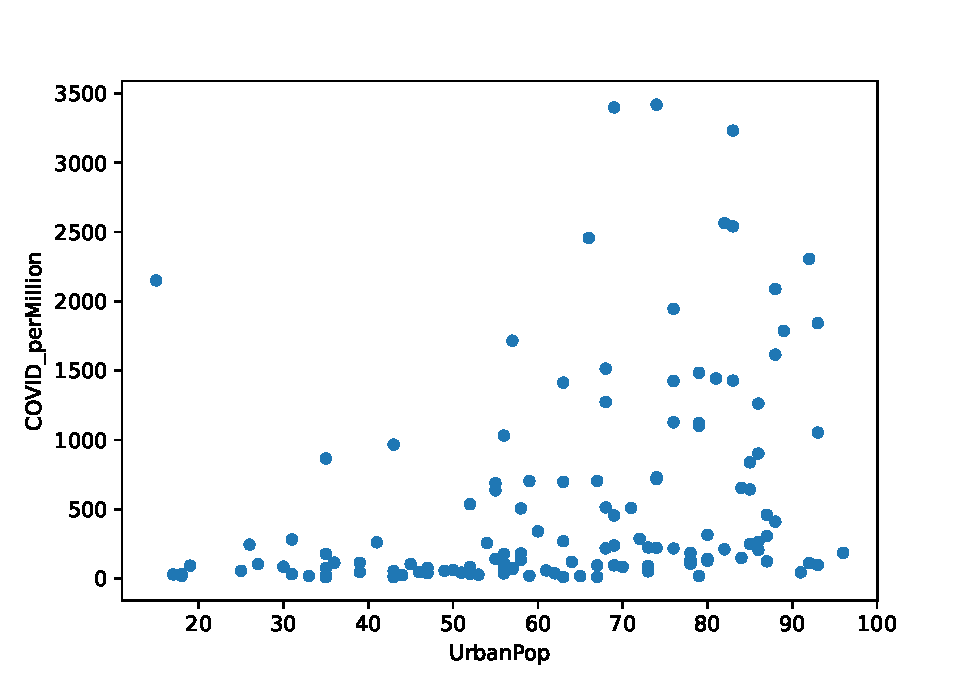
\includegraphics{_main_files/figure-latex/unnamed-chunk-124-15.pdf}

A pontdiagramon azt vehetjük észre, hogy az egymillió főre jutó COVID esetszám jobbra elnyúló eloszlása miatt jelenlévő felfelé kiugró értékek befolyásolják a két ismérv kapcsolatát. A kilógóan magas esetszámok miatt úgy tűnik, mintha az 500 alatti esetszámú országokban nem is lenne kapcsolat a két ismérv között.
A városi népesség arányával nincsenek ilyen problémák, mivel annak eloszlása közel szimmetrikus.

A két ismérv/oszlop eloszlásáról írtakat a hisztogramokon is meg lehet lesni.

Az egymillió főre jutó esetszám hisztogramja, ami elég jobbra elnyúló.

\begin{Shaded}
\begin{Highlighting}[]
\NormalTok{corona\_extended.COVID\_perMillion.hist()}
\end{Highlighting}
\end{Shaded}

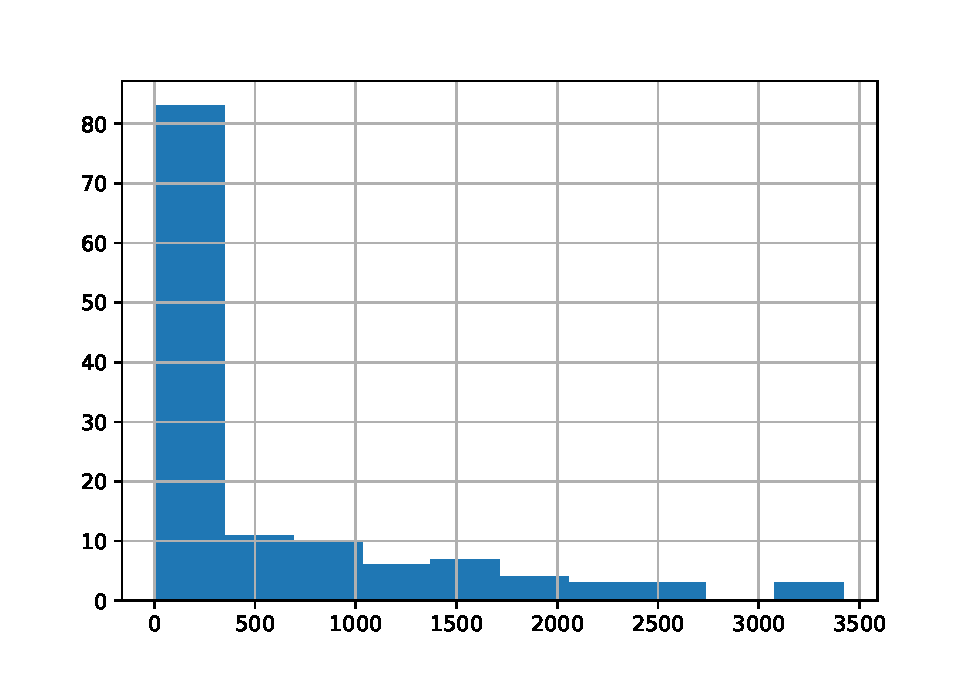
\includegraphics{_main_files/figure-latex/unnamed-chunk-125-17.pdf}

És a városi népesség arányáé, ami szimmetrikusabb egy fokkal, de némileg inkább balra elnyúló. A lényeg, hogy ezen nem segít a logaritmus. :)

\begin{Shaded}
\begin{Highlighting}[]
\NormalTok{corona\_extended.UrbanPop.hist()}
\end{Highlighting}
\end{Shaded}

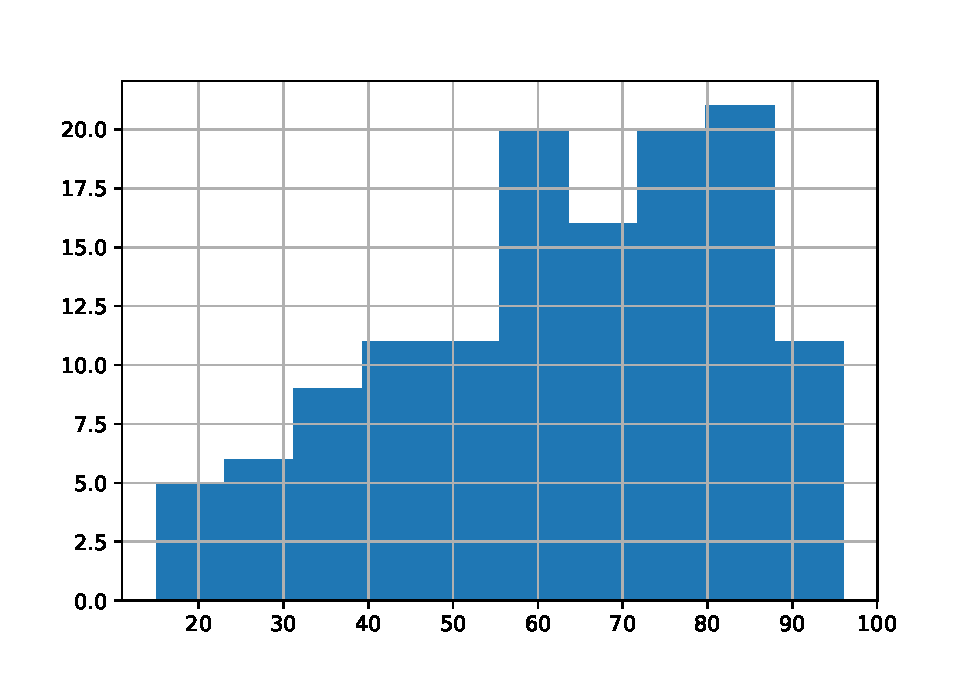
\includegraphics{_main_files/figure-latex/unnamed-chunk-126-19.pdf}

A kiugró értékek hatását, és az \textbf{eloszlás jobbra elnyúlóból közel szimmetrikussá alakítását logaritmussal} lehet elérni.

Készítsük is el a \textbf{COVID\_perMillion} oszlop természetes alapú logaritmusát egy új oszlopban a data frame-n belül.

\begin{Shaded}
\begin{Highlighting}[]
\NormalTok{corona\_extended[}\StringTok{\textquotesingle{}log\_COVID\_perMillion\textquotesingle{}}\NormalTok{] }\OperatorTok{=}\NormalTok{ np.log(corona\_extended[}\StringTok{\textquotesingle{}COVID\_perMillion\textquotesingle{}}\NormalTok{])}
\end{Highlighting}
\end{Shaded}

Ezek után lessünk rá az új oszlop hisztogramjára:

\begin{Shaded}
\begin{Highlighting}[]
\NormalTok{corona\_extended.log\_COVID\_perMillion.hist()}
\end{Highlighting}
\end{Shaded}

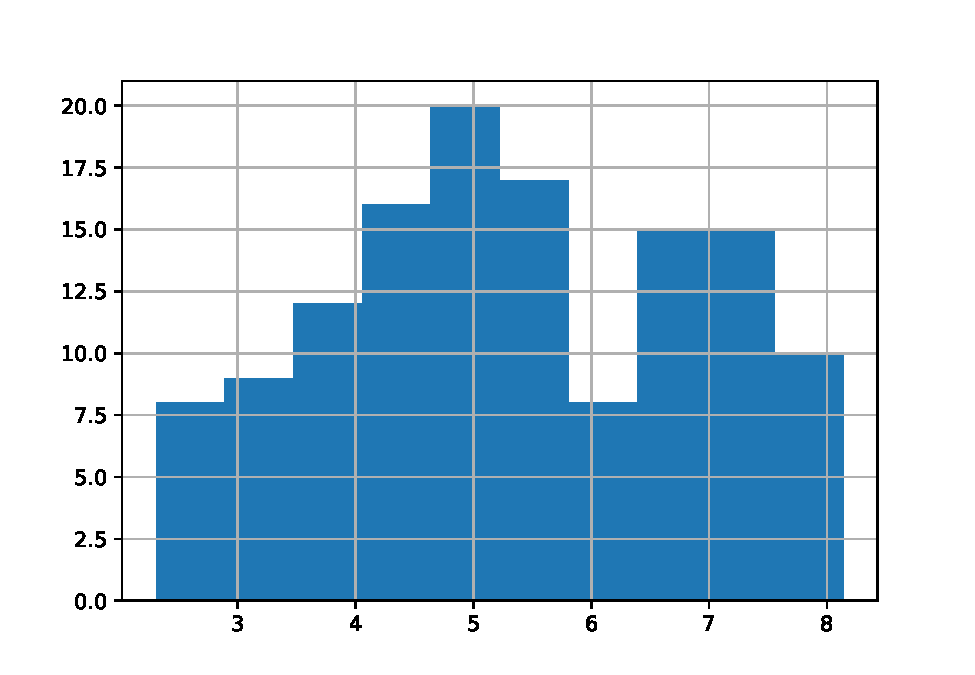
\includegraphics{_main_files/figure-latex/unnamed-chunk-128-21.pdf}

Sokkal szebb! :) Legalábbis szimmetria szempontjából biztos. Viszont van benne azért egy kétmóduszú jelleg. Ez azt jelenti, hogy van az országoknak egy jelentősebb csoportja, ahol emelkedettebb a népességarányos COVID esetszám, mint az országok többségében, akik az alacsonyabb értéktartományban lévő ``első móduszt'' adják.

A korreláció az esetszám logaritmusa és a városi népesség aránya között pedig feljavul. Abszolút értékben több, mint \(0.1\) egységet emelkedik a korreláció, ami nem elhanyagolható mértéjű javulás. :) Most a korrelációs mátrixból kivesszük a \textbf{PopDensity}-t is, hogy áttekinthetőbb legyen.

\begin{Shaded}
\begin{Highlighting}[]
\NormalTok{corona\_extended.loc[:,}\OperatorTok{\textasciitilde{}}\NormalTok{corona\_extended.columns.isin([}\StringTok{\textquotesingle{}Country\textquotesingle{}}\NormalTok{, }\StringTok{\textquotesingle{}COVID\_Cases\textquotesingle{}}\NormalTok{, }\StringTok{\textquotesingle{}Pop\textquotesingle{}}\NormalTok{, }\StringTok{\textquotesingle{}PopDensity\textquotesingle{}}\NormalTok{])].corr()}
\end{Highlighting}
\end{Shaded}

\begin{verbatim}
##                       UrbanPop  COVID_perMillion  log_COVID_perMillion
## UrbanPop              1.000000          0.341160              0.464379
## COVID_perMillion      0.341160          1.000000              0.826654
## log_COVID_perMillion  0.464379          0.826654              1.000000
\end{verbatim}

A korreláció abszolút értékében bekövetkezett javulás oka szépen látható a pontdiagramon: nincsenek már olyan durva outlierek a pontdiagramon. A pontokra nagyobb pontossággal illeszthető egy képzeletbeli egyenes a teljes tartományon nem csak az 500 feletti egymilliófőre vetített esetszámmal bíró országokban.

\begin{Shaded}
\begin{Highlighting}[]
\NormalTok{corona\_extended.plot.scatter(x}\OperatorTok{=}\StringTok{"UrbanPop"}\NormalTok{, y}\OperatorTok{=}\StringTok{"log\_COVID\_perMillion"}\NormalTok{)}
\end{Highlighting}
\end{Shaded}

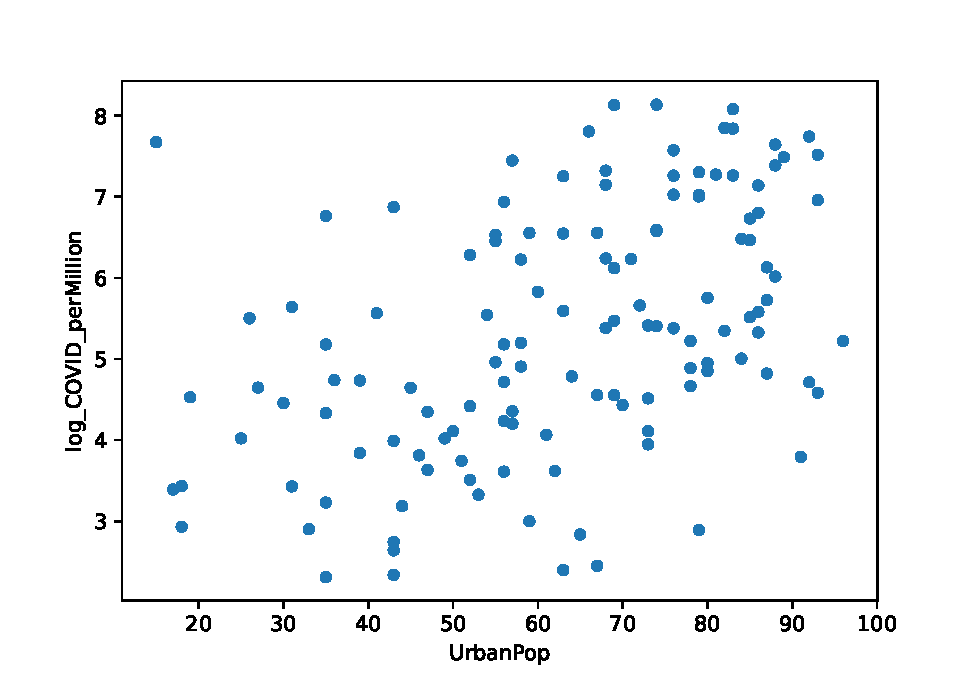
\includegraphics{_main_files/figure-latex/unnamed-chunk-130-23.pdf}

Annyit lehet látni, hogy van egy ország, aminek hatalmas az egymillió főre jutó COVID esetszáma az elég alacsony, \(20\%\) alatti városi népesség arányához képest. Jó lenne rájönni mi ez az ország!

Ehhez csináljunk egy olyan verziót az előző pontdiagramból, amin minden ponton szerepel, hogy az melyik országot jelöli.

Ennek elkészítéséhez felhasználunk egy \texttt{enumerate} névre hallgató függvényt. Ha ezt a függvényt ráeresztjük a \textbf{Country} oszlopra a data frame-ben, és az eredményt egy \texttt{for} ciklussal bejárjuk, akkor igazából két listát is bejárunk prhuzamosan:

\begin{itemize}
\tightlist
\item
  Egyet, ami az ország sorszámát mutatja a data frame-ben \(0\)-tól indexszelve. Ezt hívom én \texttt{sorszám}-nak.
\item
  A másik listában pedig az országnevek vannak. Ez a kódban \texttt{szöveg}-nek becézem.
\end{itemize}

Fontos, hogy a két listát bejáró változó neve teljesen tetszőleges, akár ``kismacska'' és ``gumimaci'' is lehetnének. :)

\begin{Shaded}
\begin{Highlighting}[]
\ControlFlowTok{for}\NormalTok{ sorszám, szöveg }\KeywordTok{in} \BuiltInTok{enumerate}\NormalTok{(corona\_extended.Country):}
   \BuiltInTok{print}\NormalTok{(sorszám)}
   \BuiltInTok{print}\NormalTok{(szöveg)}
\end{Highlighting}
\end{Shaded}

\begin{verbatim}
## 0
## Afghanistan
## 1
## Albania
## 2
## Algeria
## 3
## Antigua and Barbuda
## 4
## Argentina
## 5
## Armenia
## 6
## Australia
## 7
## Austria
## 8
## Azerbaijan
## 9
## Bahamas
\end{verbatim}

És ez így folytatódik tovább a data frame összes sorára, csak most ide nem íratom ki a több mint 100 értéket. :)

Na, ezt az \texttt{enumerate}-t használó \texttt{for} ciklust úgy hasznosítjuk, hogy először egy külön \texttt{fig} című objektumba elmentjk az alap pontdiagramos ábrát, amit az előbb is megcsináltunk.
Aztán elindítjuk ezt a \texttt{for} ciklust az \texttt{enumerate} alapján, és a cikluson belül használjuk a \texttt{fig} objektum \texttt{annotate} metódusát, ami a pontok feliratozását valósítja meg. A metódus paramétereiben megadom először, hogy az aktuális \texttt{szöveg}-et, azaz az országnevet rakja fel, mint felirat.
A következő paraméter, ami zárójelben van az csak optikai tuning. Ott azt csinálom, hogy az \(x,y\) koordinátáknak megfelelő oszlopok konkrét, pontdiagramon lévő koordinátáit kérdezem le az oszlopok \texttt{iat} tulajdonságában. Ez két lista, így mindig a \emph{sorszámadik} elemét nézem a cikluson belül. Ezen koordináták közül a diagram \(x\) tengelyét adó \textbf{UrbanPop}-ét eltolom \(0.05\)-tel. Így a pont felirata nem a pont középpontjában kezdődik, hanem attól \(0.05\) egységgel jobbra. Így olvashatóbb lesz a cucc. :) Nyilván a felirat \(y\) koordinátáját is tudnám itt szabályozni, és kedvem szerint fel-le rakni a felirat kezdőpontját, de erre itt nincs szükség, így az \texttt{annotate} paraméterben ezt a koordinátát csak csak változatlanul átadom.

Na, és lássuk is ezt a csodát működés közben! A kód végén egy \texttt{plt.show()} utasítással lehet a diagramot láthatóvá is tenni.

\begin{Shaded}
\begin{Highlighting}[]
\NormalTok{fig }\OperatorTok{=}\NormalTok{ corona\_extended.plot.scatter(x}\OperatorTok{=}\StringTok{"UrbanPop"}\NormalTok{, y}\OperatorTok{=}\StringTok{"log\_COVID\_perMillion"}\NormalTok{)}

\ControlFlowTok{for}\NormalTok{ sorszám, szöveg }\KeywordTok{in} \BuiltInTok{enumerate}\NormalTok{(corona\_extended.Country):}
\NormalTok{   fig.annotate(szöveg, (corona\_extended.UrbanPop.iat[sorszám]}\OperatorTok{+}\FloatTok{0.05}\NormalTok{, corona\_extended.log\_COVID\_perMillion.iat[sorszám]))}

\NormalTok{plt.show()}
\end{Highlighting}
\end{Shaded}

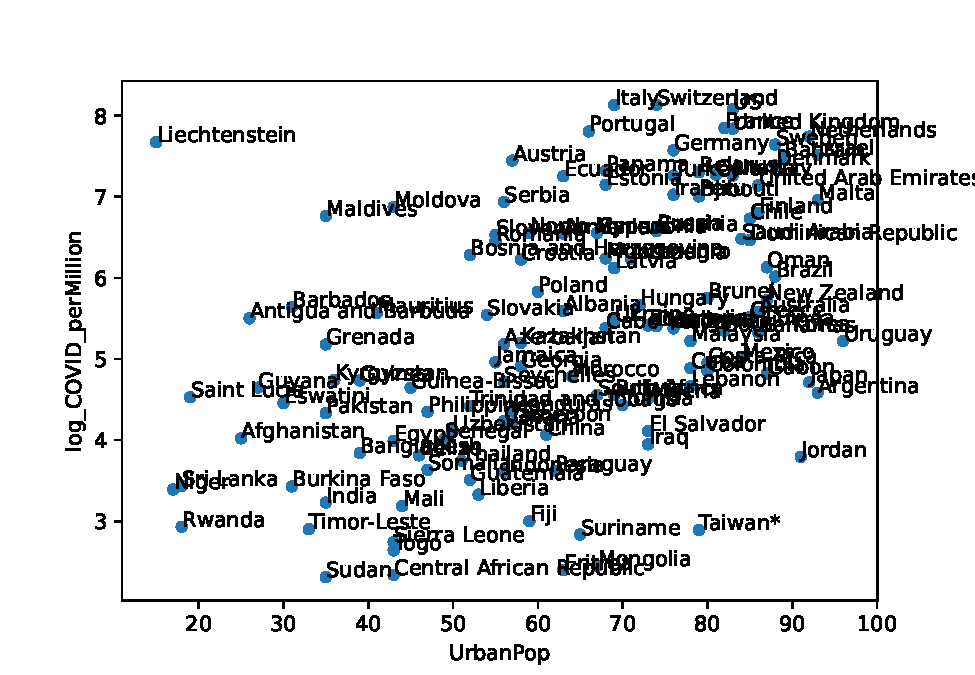
\includegraphics{_main_files/figure-latex/unnamed-chunk-133-25.pdf}

E voilá: a gyanús kis államunk a magas esetszámával a kis városi népesség arány ellenére \emph{Lichtenstein}! :) Érdekes észrevenni még, hogy pl. Taiwan elég jól áll: a városi népesség arányához képest elég alacsony az esetszáma! Magyarország, ha jól szemmelverjük, akkor látható, hogy gyakorlatilag pont a fő csapásirány közepén van kb: pont annyi nagyjából az esetszáma, amennyi a városi népesség aránya alapján ``lennie kéne''. :)

\section*{Gyakorló feladatok}\label{gyakorluxf3-feladatok}
\addcontentsline{toc}{section}{Gyakorló feladatok}

\begin{enumerate}
\def\labelenumi{\arabic{enumi}.}
\tightlist
\item
  Olvassuk be az index\_2019\_-\_pour\_import\_1\_1.csv nevű fájlt, és mentsük el a beolvasott adatokat egy \textbf{PressLiberty} nevű data frame-be!

  \begin{itemize}
  \tightlist
  \item
    Vigyázat! A fájlban tizedesvesszők vannak tizedes pont helyett! Használni kell a \texttt{read\_csv} függvény \texttt{decimal} paraméterét! Meg kell a paraméterben adni, hogy a tizedeshelyeket a \texttt{\textquotesingle{},\textquotesingle{}} karakter jelöli!
  \end{itemize}
\item
  A \textbf{PressLiberty} data frame-ből csak az angol országnév (\textbf{EN\_country}) és a 2019-es sajtószabadsági index (\textbf{Score 2019}) oszlopkra lesz szükségünk. A sajtószabadsági indexben az alacsonyabb érték jelent szabadabb sajtót egy országban. A többi változót töröljuk ki a data frame-ből!
\item
  A szűkített \textbf{PressLiberty} data frame oszlopainak neve legyen \textbf{Country} és \textbf{PressLiberty}!
\item
  Változtassuk meg az Egyesült Államok nevét ``\emph{United States}''-ről ``\emph{US}''-re a \textbf{PressLiberty} data frame-ben, hogy az összeköthető legyen a \textbf{corona\_extended} data frame-el az országneveken keresztül!
\item
  Inner Join művelet segítségével vezessük át a sajtószabadsági index vonatkozó adatokat a \textbf{corona\_extended} data frame-be!
\item
  Ábrázoljuk a \textbf{corona\_extended} data frame-ben a kapcsolatot a \textbf{log\_COVID\_perMillion} és \textbf{PressLiberty} ismérvek között pontdiagramon! Értelmezze röviden szövegesen is a kapcsolatot! Logikus-e a kapcsolat iránya?
\item
  Vizsgáljuk meg a \textbf{PressLiberty} eloszlását hisztogramon!
\item
  Adjuk hozzá a \textbf{corona\_extended} data frame-hez a \textbf{PressLiberty} logaritmusát \textbf{log\_PressLiberty} néven!
\item
  Nézzük meg a korrelációs mátrixot a \textbf{log\_COVID\_perMillion}, \textbf{PressLiberty} és \textbf{log\_PressLiberty} ismérvek között! Volt-e értelme a logaritmus alkalmazásának? Válaszát röviden indokolja!
\item
  Ábrázoljuk a \textbf{corona\_extended} data frame-ben a kapcsolatot a \textbf{COVID\_perMillion} logaritmusa és a \textbf{PressLiberty} logaritmusa között pontdiagramon! Az egyes pontokon szerepeljen az országok neve is!

  \begin{itemize}
  \tightlist
  \item
    Van-e olyan ország, amelyik a két ismérv kapcsolatát leíró általános tendenciához képest eltérően viselkedik? Válaszát röviden indokolja!
  \end{itemize}
\end{enumerate}

\section*{Gyakorló feladatok megoldása}\label{gyakorluxf3-feladatok-megolduxe1sa}
\addcontentsline{toc}{section}{Gyakorló feladatok megoldása}

\subsection*{1. feladat}\label{feladat}
\addcontentsline{toc}{subsection}{1. feladat}

\begin{Shaded}
\begin{Highlighting}[]
\NormalTok{PressLiberty }\OperatorTok{=}\NormalTok{ pd.read\_csv(}\StringTok{\textquotesingle{}index\_2019\_{-}\_pour\_import\_1\_1.csv\textquotesingle{}}\NormalTok{, decimal}\OperatorTok{=}\StringTok{\textquotesingle{},\textquotesingle{}}\NormalTok{)}
\NormalTok{PressLiberty.info()}
\end{Highlighting}
\end{Shaded}

\begin{verbatim}
## <class 'pandas.core.frame.DataFrame'>
## RangeIndex: 180 entries, 0 to 179
## Data columns (total 14 columns):
##  #   Column            Non-Null Count  Dtype  
## ---  ------            --------------  -----  
##  0   ISO               180 non-null    object 
##  1   Rank2019          180 non-null    int64  
##  2   FR_Country        180 non-null    object 
##  3   EN_country        180 non-null    object 
##  4   ES_country        180 non-null    object 
##  5   Score A           180 non-null    float64
##  6   Sco Exa           180 non-null    float64
##  7   Score 2019        180 non-null    float64
##  8   Progression RANK  180 non-null    int64  
##  9   Rank 2018         180 non-null    int64  
##  10  Score 2018        180 non-null    float64
##  11  Zone              180 non-null    object 
##  12  AR_country        180 non-null    object 
##  13  FA_country        180 non-null    object 
## dtypes: float64(4), int64(3), object(7)
## memory usage: 19.8+ KB
\end{verbatim}

\subsection*{2. feladat}\label{feladat-1}
\addcontentsline{toc}{subsection}{2. feladat}

\begin{Shaded}
\begin{Highlighting}[]
\NormalTok{PressLiberty }\OperatorTok{=}\NormalTok{ PressLiberty.loc[:,[}\StringTok{\textquotesingle{}EN\_country\textquotesingle{}}\NormalTok{, }\StringTok{\textquotesingle{}Score 2019\textquotesingle{}}\NormalTok{]]}
\NormalTok{PressLiberty.info()}
\end{Highlighting}
\end{Shaded}

\begin{verbatim}
## <class 'pandas.core.frame.DataFrame'>
## RangeIndex: 180 entries, 0 to 179
## Data columns (total 2 columns):
##  #   Column      Non-Null Count  Dtype  
## ---  ------      --------------  -----  
##  0   EN_country  180 non-null    object 
##  1   Score 2019  180 non-null    float64
## dtypes: float64(1), object(1)
## memory usage: 2.9+ KB
\end{verbatim}

\subsection*{3. feladat}\label{feladat-2}
\addcontentsline{toc}{subsection}{3. feladat}

\begin{Shaded}
\begin{Highlighting}[]
\NormalTok{PressLiberty.columns }\OperatorTok{=}\NormalTok{ [}\StringTok{\textquotesingle{}Country\textquotesingle{}}\NormalTok{, }\StringTok{\textquotesingle{}PressLiberty\textquotesingle{}}\NormalTok{]}
\NormalTok{PressLiberty.info()}
\end{Highlighting}
\end{Shaded}

\begin{verbatim}
## <class 'pandas.core.frame.DataFrame'>
## RangeIndex: 180 entries, 0 to 179
## Data columns (total 2 columns):
##  #   Column        Non-Null Count  Dtype  
## ---  ------        --------------  -----  
##  0   Country       180 non-null    object 
##  1   PressLiberty  180 non-null    float64
## dtypes: float64(1), object(1)
## memory usage: 2.9+ KB
\end{verbatim}

\subsection*{4. feladat}\label{feladat-3}
\addcontentsline{toc}{subsection}{4. feladat}

\begin{Shaded}
\begin{Highlighting}[]
\NormalTok{PressLiberty[}\StringTok{\textquotesingle{}Country\textquotesingle{}}\NormalTok{] }\OperatorTok{=}\NormalTok{ PressLiberty[}\StringTok{\textquotesingle{}Country\textquotesingle{}}\NormalTok{].replace(}\StringTok{\textquotesingle{}United States\textquotesingle{}}\NormalTok{, }\StringTok{\textquotesingle{}US\textquotesingle{}}\NormalTok{)}
\end{Highlighting}
\end{Shaded}

\subsection*{5. feladat}\label{feladat-4}
\addcontentsline{toc}{subsection}{5. feladat}

\begin{Shaded}
\begin{Highlighting}[]
\NormalTok{corona\_extended }\OperatorTok{=}\NormalTok{ pd.merge(corona\_extended, PressLiberty, how}\OperatorTok{=}\StringTok{\textquotesingle{}inner\textquotesingle{}}\NormalTok{, on}\OperatorTok{=}\StringTok{\textquotesingle{}Country\textquotesingle{}}\NormalTok{)}
\NormalTok{corona\_extended.info()}
\end{Highlighting}
\end{Shaded}

\begin{verbatim}
## <class 'pandas.core.frame.DataFrame'>
## RangeIndex: 115 entries, 0 to 114
## Data columns (total 8 columns):
##  #   Column                Non-Null Count  Dtype  
## ---  ------                --------------  -----  
##  0   Country               115 non-null    object 
##  1   COVID_Cases           115 non-null    int64  
##  2   Pop                   115 non-null    int64  
##  3   PopDensity            115 non-null    int64  
##  4   UrbanPop              115 non-null    int32  
##  5   COVID_perMillion      115 non-null    float64
##  6   log_COVID_perMillion  115 non-null    float64
##  7   PressLiberty          115 non-null    float64
## dtypes: float64(3), int32(1), int64(3), object(1)
## memory usage: 6.9+ KB
\end{verbatim}

\subsection*{6. feladat}\label{feladat-5}
\addcontentsline{toc}{subsection}{6. feladat}

\begin{Shaded}
\begin{Highlighting}[]
\NormalTok{corona\_extended.plot.scatter(x}\OperatorTok{=}\StringTok{"PressLiberty"}\NormalTok{, y}\OperatorTok{=}\StringTok{"log\_COVID\_perMillion"}\NormalTok{)}
\end{Highlighting}
\end{Shaded}

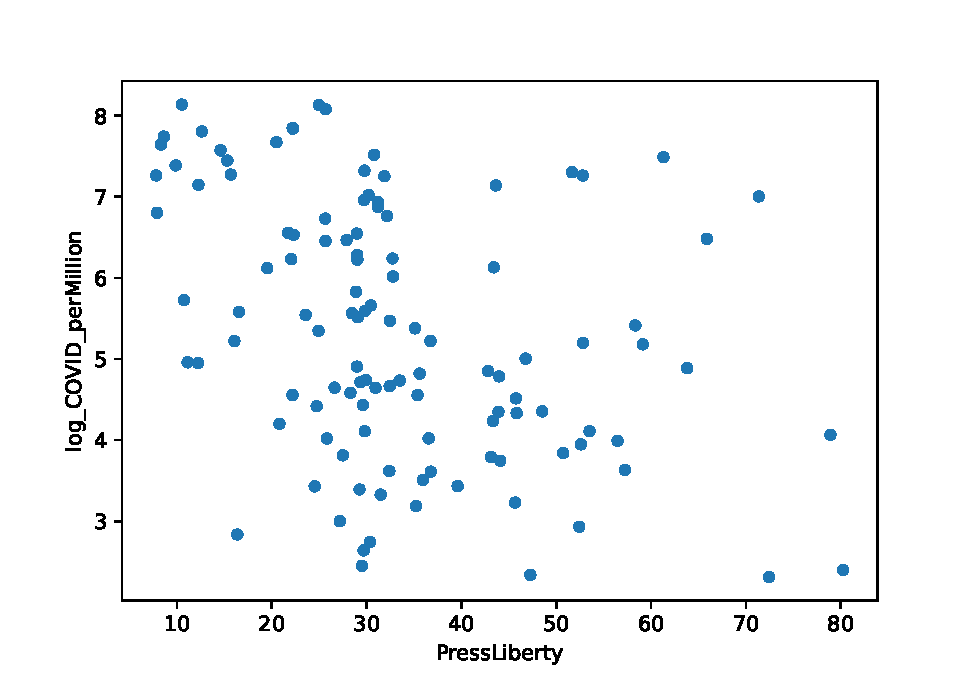
\includegraphics{_main_files/figure-latex/unnamed-chunk-139-27.pdf}

Úgy látszik, hogy a a kapcsolat ellentétes irányú: a sajtószabadsági index növekedésével jellemzően csökken az esetszám. Mivel a magasabb index jelenti a kevésbé szabad sajtót, így első olvasatra nem logikus a kapcsolat iránya: kevésbé szabad sajtóval rendelkező országokban kevesebb az esetszám egymillió főre nézve. De egy picit belegondolva lehet logikus a dolog: a szabadabb sajtóval rendelkező országok jellemzően gazdagabb országok is. Feltehetően ilyen országokban a COVID tesztelésre is több erőforrás jut.

\subsection*{7. feladat}\label{feladat-6}
\addcontentsline{toc}{subsection}{7. feladat}

\begin{Shaded}
\begin{Highlighting}[]
\NormalTok{corona\_extended.PressLiberty.hist()}
\end{Highlighting}
\end{Shaded}

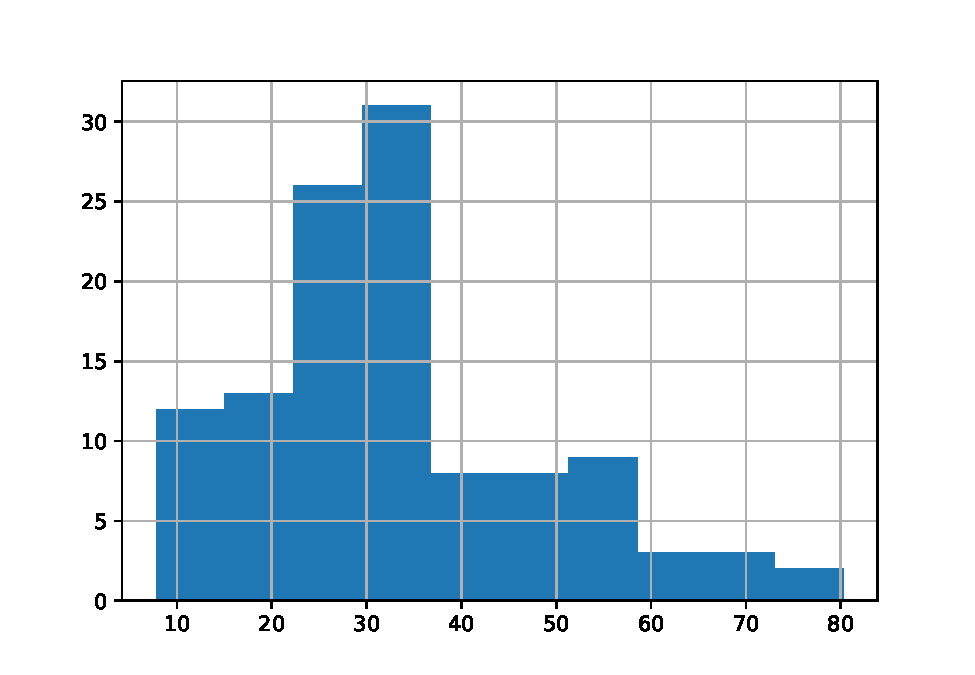
\includegraphics{_main_files/figure-latex/unnamed-chunk-140-29.pdf}

Az eloszlás némileg jobbra elnyúló, vannak felső irányban kiugró értékek. Érdemes lehet logaritmust alkalmazni az oszlopon.

\subsection*{8. feladat}\label{feladat-7}
\addcontentsline{toc}{subsection}{8. feladat}

\begin{Shaded}
\begin{Highlighting}[]
\NormalTok{corona\_extended[}\StringTok{\textquotesingle{}log\_PressLiberty\textquotesingle{}}\NormalTok{] }\OperatorTok{=}\NormalTok{ np.log(corona\_extended[}\StringTok{\textquotesingle{}PressLiberty\textquotesingle{}}\NormalTok{])}
\NormalTok{corona\_extended.info()}
\end{Highlighting}
\end{Shaded}

\begin{verbatim}
## <class 'pandas.core.frame.DataFrame'>
## RangeIndex: 115 entries, 0 to 114
## Data columns (total 9 columns):
##  #   Column                Non-Null Count  Dtype  
## ---  ------                --------------  -----  
##  0   Country               115 non-null    object 
##  1   COVID_Cases           115 non-null    int64  
##  2   Pop                   115 non-null    int64  
##  3   PopDensity            115 non-null    int64  
##  4   UrbanPop              115 non-null    int32  
##  5   COVID_perMillion      115 non-null    float64
##  6   log_COVID_perMillion  115 non-null    float64
##  7   PressLiberty          115 non-null    float64
##  8   log_PressLiberty      115 non-null    float64
## dtypes: float64(4), int32(1), int64(3), object(1)
## memory usage: 7.8+ KB
\end{verbatim}

\subsection*{9. feladat}\label{feladat-8}
\addcontentsline{toc}{subsection}{9. feladat}

\begin{Shaded}
\begin{Highlighting}[]
\NormalTok{corona\_extended.loc[:,[}\StringTok{\textquotesingle{}log\_COVID\_perMillion\textquotesingle{}}\NormalTok{, }\StringTok{\textquotesingle{}PressLiberty\textquotesingle{}}\NormalTok{, }\StringTok{\textquotesingle{}log\_PressLiberty\textquotesingle{}}\NormalTok{]].corr()}
\end{Highlighting}
\end{Shaded}

\begin{verbatim}
##                       log_COVID_perMillion  PressLiberty  log_PressLiberty
## log_COVID_perMillion              1.000000     -0.381829         -0.430291
## PressLiberty                     -0.381829      1.000000          0.944278
## log_PressLiberty                 -0.430291      0.944278          1.000000
\end{verbatim}

Volt értelme, a sajtószabadsági indexnek jobbra elnyúló az eloszlása, így a kilógó értékek hatását az egymillió főre vetített esetszámmal vett kapcsolatára tudta mérsékelni a logaritmus. Ez onnan látszódik, hogy a korreláció abszolút értékben \(0.05\) egységgel nőtt. Nem akkora a javulás, mint a városi népesség arányával vett korrelációnál tapasztaltuk, de azért észrevehető.

\subsection*{10. feladat}\label{feladat-9}
\addcontentsline{toc}{subsection}{10. feladat}

\begin{Shaded}
\begin{Highlighting}[]
\NormalTok{fig }\OperatorTok{=}\NormalTok{ corona\_extended.plot.scatter(x}\OperatorTok{=}\StringTok{"log\_PressLiberty"}\NormalTok{, y}\OperatorTok{=}\StringTok{"log\_COVID\_perMillion"}\NormalTok{)}

\ControlFlowTok{for}\NormalTok{ sorszám, szöveg }\KeywordTok{in} \BuiltInTok{enumerate}\NormalTok{(corona\_extended.Country):}
\NormalTok{   fig.annotate(szöveg, (corona\_extended.log\_PressLiberty.iat[sorszám]}\OperatorTok{+}\FloatTok{0.05}\NormalTok{, corona\_extended.log\_COVID\_perMillion.iat[sorszám]))}

\NormalTok{plt.show()}
\end{Highlighting}
\end{Shaded}

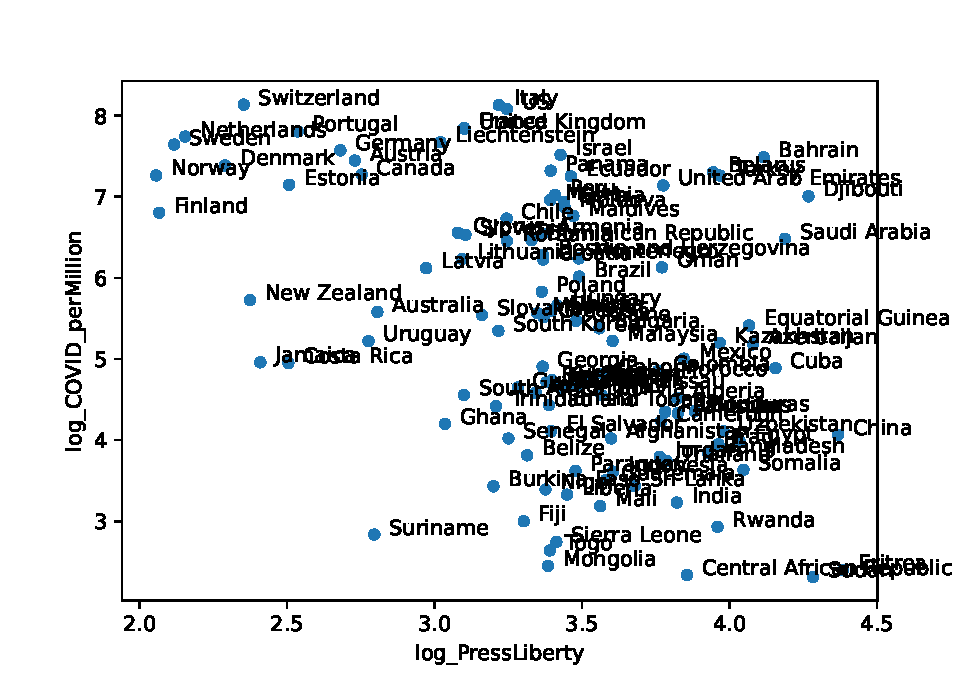
\includegraphics{_main_files/figure-latex/unnamed-chunk-143-31.pdf}

Úgy látszik, hogy pl. a dél-amerikai \emph{Suriname}-ben még a viszonylag rossz sajtószabadsági indexhez képest is kevés esettalálható egymillió főre. \emph{Bahrain}ben és \emph{Szaúd-Arábiában} viszont épp, hogy magas az esetszám a kevésbé szabad sajtó ellenére is. Itt lehet az olajvagyonból futja tesztelésre is \emph{úgymond}. :)

\chapter{Leíró Statisztika ismétlés és Valószínűségszámítás alapok}\label{leuxedruxf3-statisztika-ismuxe9tluxe9s-uxe9s-valuxf3szuxednux171suxe9gszuxe1muxedtuxe1s-alapok}

\section{Leíró statisztikai mutatók}\label{leuxedruxf3-statisztikai-mutatuxf3k}

A Stat. I. PTSD roham kiváltását kezdjük egy nagyon egyszerű kis ``Móricka példán''. Vizsgáljuk meg a TSLA.xlsx című táblában található adatokat, amik a \textbf{TESLA részvények napi záróárfolyam-változásai}t mutatják ki \textbf{dollárban} (\$) 2019 májusától 2020 májusáig.

Az Excel táblákat, amennyiben az adattáblánk első értéke az \emph{A1} cellában kezdődik és csak egy darab munkalapunk van, gond nélkül be lehet olvasni a \texttt{pandas} csomag \texttt{read\_excel} függvényével egy data frame-be. Több munkalap esetén a \texttt{read\_excel} függvény \texttt{sheet\_name} paraméterével tudjuk megadni a beolvasandó munkalap nevét stringként. Viszont ahhoz, hogy ez működőképes legyen fel kell még telepítenünk egy \texttt{openpyxl} című kiegészítő csomagot. A biztonság kedvéért ezzel a művelettel együtt rögtön importáljuk a statisztikai számításokhoz szükséges \texttt{numpy} és az ábrák megjelenítéséhez szükséges \texttt{matplotlib} csomagokat is.

\begin{Shaded}
\begin{Highlighting}[]
\NormalTok{pip install openpyxl}
\ImportTok{import}\NormalTok{ pandas }\ImportTok{as}\NormalTok{ pd}
\ImportTok{import}\NormalTok{ matplotlib.pyplot }\ImportTok{as}\NormalTok{ plt}
\ImportTok{import}\NormalTok{ numpy }\ImportTok{as}\NormalTok{ np}
\end{Highlighting}
\end{Shaded}

Ezek után pedig akkor jöhet az Excel beolvasás data frame-be!

\begin{Shaded}
\begin{Highlighting}[]
\NormalTok{Tesla }\OperatorTok{=}\NormalTok{ pd.read\_excel(}\StringTok{"TSLA.xlsx"}\NormalTok{)}

\NormalTok{Tesla.info()}
\end{Highlighting}
\end{Shaded}

\begin{verbatim}
## <class 'pandas.core.frame.DataFrame'>
## RangeIndex: 250 entries, 0 to 249
## Data columns (total 2 columns):
##  #   Column  Non-Null Count  Dtype         
## ---  ------  --------------  -----         
##  0   Dátum   250 non-null    datetime64[ns]
##  1   TESLA   250 non-null    float64       
## dtypes: datetime64[ns](1), float64(1)
## memory usage: 4.0 KB
\end{verbatim}

\begin{Shaded}
\begin{Highlighting}[]
\NormalTok{Tesla.head()}
\end{Highlighting}
\end{Shaded}

\begin{verbatim}
##        Dátum      TESLA
## 0 2019-05-07  -8.279998
## 1 2019-05-08  -2.220002
## 2 2019-05-09  -2.860000
## 3 2019-05-10  -2.459992
## 4 2019-05-13 -12.510009
\end{verbatim}

Láthatjuk, hogy két oszlopunk van: a dátum és a részvény árváltozása az adott napon az előző napi záróárfolyamhoz képest a \textbf{TESLA} oszlopban. Tehát 2019.05.07-én egy Tesla részvény kb. \(8.3\) dollárral ért kevesebbet a nap végére, mint amennyit 2019.05.06-án ért nap végén. Ellenben 05.13-án már \(12.5\) dollárral ér kevesebbet, mint előző nap, 05.12-én. Az \texttt{info} metódus alapján \(N=250\) napnyi ilyen adatunk van, ami nagyjából meg is egyezik egy évben a tőzsdei kereskedési napok számával.

Nos, az első öt vizsgált nap alapján nem lennék Elon Musk helyében, elég szép mínuszokat produkál a részvénye. De lássuk, hogy a leíró statisztikai mutatók mit árulnak el, hogyan is teljesített ez a csodacég a teljes vizsgált 1 éves időtartamban! Vessük át be a data frame \texttt{describe} metódusát!

\begin{Shaded}
\begin{Highlighting}[]
\NormalTok{Tesla.describe()}
\end{Highlighting}
\end{Shaded}

\begin{verbatim}
##                             Dátum       TESLA
## count                         250  250.000000
## mean   2019-11-02 15:56:09.600000    1.783920
## min           2019-05-07 00:00:00 -152.359986
## 25%           2019-08-05 06:00:00   -3.770005
## 50%           2019-10-31 12:00:00    1.420006
## 75%           2020-02-02 06:00:00    6.957486
## max           2020-05-01 00:00:00  129.429993
## std                           NaN   27.192611
\end{verbatim}

Lássuk hát milyen sztorit mesélnek a kiszámított mutatóink!

\begin{itemize}
\tightlist
\item
  Úgy látszik, hogy abszolút értékben a legnagyobb veszteség (\(-152\$\)) némileg nagyobb, mint a legnagyobb nyereség (\(+129\$\)).
\item
  Ugyanakkor, egy átlagos napon nagyjából jól járunk egy Tesla részvénnyel, mert kb. \(\mu=\bar{Y}=1.8\$\)-al növeli értékét.
\item
  Viszont, marha nagy a rizikó a rendszerben, mert a szórás (angolul \emph{standard deviation}, rövidítve \texttt{std}) alapján egy véletlenszerűen kiválasztott napon az árváltozás az \(\sigma=1.8\$\)-os átlagtól várhatóan \(\pm27.2\$\)-al térhet el. Azaz az árváltozások várható ingadozása az átlagos nyereségnek mintegy \(V=\frac{\sigma}{\mu}=\frac{27.2}{1.8}=15.1\)-szerese! (\emph{relatív szórás})
\item
  A medián árváltozás alapján azt mondhatjuk el, hogy a vizsgált időszakban a napok felében az elérhető maximális nyereség \(Me=1.42\$\), míg a napok másik felében a nyereség pedig legalább ennyi.
\item
  Az alsó kvartilis alapján a kereskedési napok legrosszabb \(\frac{1}{4}\)-ében a veszteség nagyobb, mint \(3.77\$\). Másképp: az árváltozás a napok negyedében kisebb, mint \(Q_1=-3.77\$\).
\item
  A napjaink legjobb \(25\%\)-ban pedig a nyereség legalább \(Q_3=6.96\$\)
\end{itemize}

Ha a fenti megállapításokat összenézzük, akkor arra juthatunk, hogy az \textbf{árváltozások eloszlása kb. szimmetrikus} lehet, egy \textbf{enyhe jobbra elnyúlással}. A \textbf{szimmetria mellett szól}, hogy az átlag nem nagyon tér el a mediántól (tehát a kilógó értékekre érzékeny átlag nem nagyon mozog el a kilógó értékekre robusztus felezőponttól), és a medián nagyjából egyenlő távolságra van az alsó és felső kvartilisektől (szóval az \(50\%\)-os pont a gyakoriságok szerint, értékekben is kb. a \(25\%\) és \(75\%\)-os pontok közepén helyezkedik el). Ellenben az \textbf{enyhe jobbra elnyúlás mellett érvel}, hogy azért mégis az átlag enyhén nagyobb mediánnál (tehát a felfelé kilógó értékek kicsit felfelé húzzák az átlagértéket a felezőponthoz képest), és a medián enyhén közelebb van az alsó kvartilishez, mint a felsőhöz (tehát az adatok többsége egy kicsit inkább az értéktartomány aljára koncentrálódik \(\rightarrow\) a kisebb értékből egy kicsit több van). De ezek tényleg nagyon enyhe eltérések. Sőt, \textbf{akár még a balra elnyúló eloszlás felé is lehet érvelni} azzal, hogy \(Q_3\) közelebb van a maximumhoz, mint \(Q_1\) a minimumhoz, tehát a \emph{felső} \(25\%\)-ban lévő értékek ``kevésbé húznak szét'', nem annyira kilógóak, mint az \emph{alsó} \(25\%\)-ban lévők.

\subsection{Hisztogram és Alakmutatók}\label{hisztogram-uxe9s-alakmutatuxf3k}

Az előző bekezdés dilemmáit leginkább \textbf{egy hisztogram segítségével tudnánk tisztázni}. A \textbf{hisztogramhoz} viszont szükségünk van egy \textbf{osztályközös gyakorisági táblára}, hiszen az árfolyamváltozások értékkészlete elég tág. Az osztályközöket vegyük egyenlő hosszúra. Ezek után már csak azt kell eldöntenünk, hogy \textbf{hány osztályközt} hozzunk létre! Ezt ugye Stat. I-ben legtöbbször a \textbf{``\(2^k\) szabállyal''} adtuk meg. Tehát az osztályközök száma a legkisebb olyan \(k\) szám, amire igaz az, hogy \(2^k \geq N\), ahol \(N\) az adataink elemszáma. Azt láttuk a \texttt{describe} eredményéből is pl., hogy \(N=250\). Ez alapján pedig a keresett \(k\) az \(8\) lesz, mert \(k=8:2^8 = 256 >250\), ám \(k=7:2^7=128 < 250\). Ha valaki ezt pitonul szeretné kiszámolni arra figyeljen, hogy ott a hatványozás jele a \texttt{**}.

\begin{Shaded}
\begin{Highlighting}[]
\DecValTok{2}\OperatorTok{**}\DecValTok{7}
\end{Highlighting}
\end{Shaded}

\begin{verbatim}
## 128
\end{verbatim}

\begin{Shaded}
\begin{Highlighting}[]
\DecValTok{2}\OperatorTok{**}\DecValTok{8}
\end{Highlighting}
\end{Shaded}

\begin{verbatim}
## 256
\end{verbatim}

Akkor hát nézzük meg a 8 egyenlő hosszú osztályközzel bíró gyakorisági tábla alapján készített hisztogramot.

\begin{Shaded}
\begin{Highlighting}[]
\NormalTok{Tesla.TESLA.hist(bins }\OperatorTok{=} \DecValTok{8}\NormalTok{)}
\end{Highlighting}
\end{Shaded}

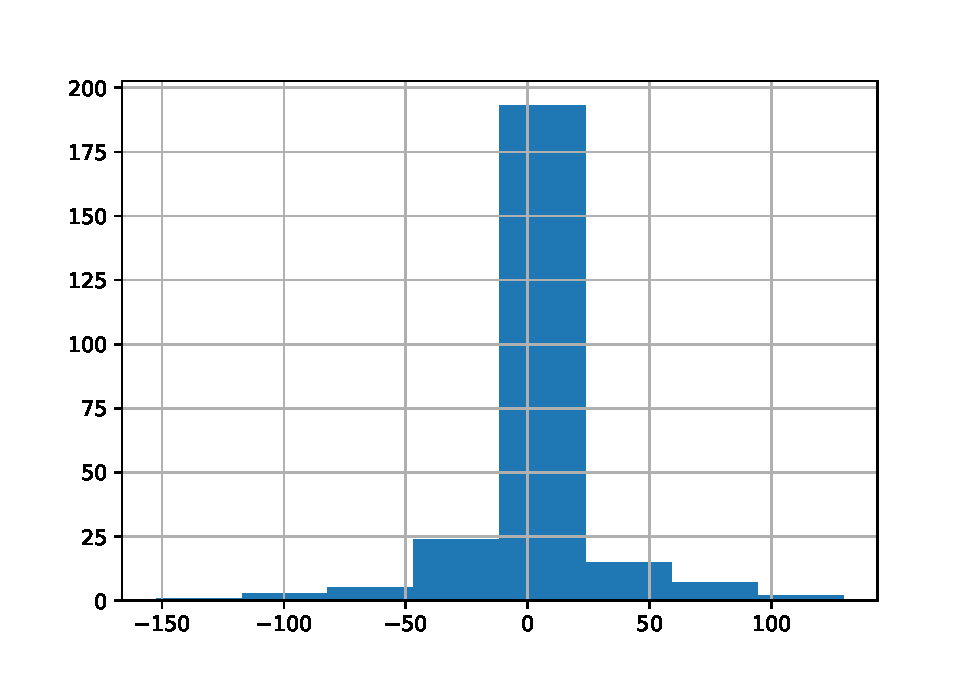
\includegraphics{_main_files/figure-latex/unnamed-chunk-149-33.pdf}

Nagyon szép, tényleg sac/kb szimmetrikus az eloszlás: középen, az \(1.8\$\)-os átlag körül csoportosul a legtöbb elem, és az ennél kisebb és nagyobb értékekből arányosan kevesebb van. Bár némileg kicsit csúcsosnak néz ki az eloszlás: a középső, átlag körüli, leggyakoribb értéktartományra koncentrálódik az adatok legnagyobb része, kb. \(190\) nap értéke az \(N=250\)-ből. Lássuk mi mondanak erről az \(\alpha_3, \alpha_4\) \textbf{alakmutatók}!

Az \(\alpha_3\) \textbf{aszimmetria mutató} Pythonban egy data frame oszlop \texttt{skew} metódusával, míg az \(\alpha_4\) \textbf{csúcsossági muató} az oszlop \texttt{skew} metódusával számítható.

\begin{Shaded}
\begin{Highlighting}[]
\NormalTok{Tesla.TESLA.skew()}
\end{Highlighting}
\end{Shaded}

\begin{verbatim}
## -0.5253045816998407
\end{verbatim}

\begin{Shaded}
\begin{Highlighting}[]
\NormalTok{Tesla.TESLA.kurt()}
\end{Highlighting}
\end{Shaded}

\begin{verbatim}
## 9.086855960563858
\end{verbatim}

Az \(\alpha_3\) értéke nagyon picit negatív, így enyhe balra elnyúlást jelez, de a hisztogram alapján látszik, hogy ez tényleg nagyon gyenge tendencia. Ez ugyebár abból adódik hogy \(Q_3\) közelebb van a maximumhoz, mint \(Q_1\) a minimumhoz. Tehát ezt a nagyon enyhe ``balra elnyúlást'' csak a maximum némileg kilógó viselkedése okozza, amire az \(\alpha_3\) ugyebár érzékeny, hiszen az átlag (\(\mu\)) alapján számoljuk őt ki (átlag körüli harmadik momentum).
Ellenben az \(\alpha_4=+9.09\)-es nagyon erősen pozitív értéke egyértelműen csúcsos eloszlás mutat, amit gyönyörűen látunk is a hisztogramon.

\subsection{Gyakorisági tábla lekérése}\label{gyakorisuxe1gi-tuxe1bla-lekuxe9ruxe9se}

Ha szeretnénk \textbf{megtekinteni a hisztogram mögött lakó osztályközös gyakorisági táblát}, akkor a dolgunk annyi, hogy a \texttt{hist} metódus helyett a \texttt{numpy} csomag \texttt{histogram} függvényével készítsük el a hisztogramot, és az eredményt mentsük el egy külön objektumba. A \texttt{histogram} függvény első paramétere az a data frame oszlop, amiből hisztogramot készítenénk, míg a második paramétere a \texttt{bins}, ami ugyan az, mint a data frame \texttt{hist} metódusában. Az elmentett eredményt data frame-é konvertáljuk a \texttt{pandas} csomag \texttt{DataFrame} függvénye segítségével, majd az eredményt transzponáljuk (alias 90 fokkal elforgatjuk) a data frame-k \texttt{transpose} metódusa segítségével.

\begin{Shaded}
\begin{Highlighting}[]
\NormalTok{gyaktábla }\OperatorTok{=}\NormalTok{ np.histogram(Tesla.TESLA, bins }\OperatorTok{=} \DecValTok{8}\NormalTok{)}
\NormalTok{gyaktábla }\OperatorTok{=}\NormalTok{ pd.DataFrame(gyaktábla).transpose()}
\NormalTok{gyaktábla}
\end{Highlighting}
\end{Shaded}

\begin{verbatim}
##        0           1
## 0    1.0 -152.359986
## 1    3.0 -117.136239
## 2    5.0  -81.912491
## 3   24.0  -46.688744
## 4  193.0  -11.464996
## 5   15.0   23.758751
## 6    7.0   58.982498
## 7    2.0   94.206246
## 8    NaN  129.429993
\end{verbatim}

Amit kaptunk az egy olyan tábla, aminek az \textbf{első oszlopa a gyakoriságok} értéke, míg a \textbf{második az adott osztályköz alsó határa}. Ezért van az utolsó sorban üres (\texttt{NaN}) érték, mert az ottani alsó határ az a vizsgált ismérvünk (árváltozásunk) maximuma, ami fölött természetesen már nincs érték.

Nevezzük át tartalmuknak megfelelően az oszlopokat, majd a \texttt{shift} metódus segítségével rakjuk be a táblába az adott osztályközök felső határait is. Itt a a \texttt{shift} metódusnál az alapelv, hogy az adott osztályköz felső határa nem más, mint a következő sor alsó határa.

\begin{Shaded}
\begin{Highlighting}[]
\NormalTok{gyaktábla.columns }\OperatorTok{=}\NormalTok{ [}\StringTok{\textquotesingle{}Gyakoriság\textquotesingle{}}\NormalTok{, }\StringTok{\textquotesingle{}AlsóHatár\textquotesingle{}}\NormalTok{]}
\NormalTok{gyaktábla.info()}
\end{Highlighting}
\end{Shaded}

\begin{verbatim}
## <class 'pandas.core.frame.DataFrame'>
## RangeIndex: 9 entries, 0 to 8
## Data columns (total 2 columns):
##  #   Column      Non-Null Count  Dtype  
## ---  ------      --------------  -----  
##  0   Gyakoriság  8 non-null      float64
##  1   AlsóHatár   9 non-null      float64
## dtypes: float64(2)
## memory usage: 276.0 bytes
\end{verbatim}

\begin{Shaded}
\begin{Highlighting}[]
\NormalTok{gyaktábla[}\StringTok{\textquotesingle{}FelsőHatár\textquotesingle{}}\NormalTok{] }\OperatorTok{=}\NormalTok{ gyaktábla.AlsóHatár.shift(}\OperatorTok{{-}}\DecValTok{1}\NormalTok{)}
\NormalTok{gyaktábla}
\end{Highlighting}
\end{Shaded}

\begin{verbatim}
##    Gyakoriság   AlsóHatár  FelsőHatár
## 0         1.0 -152.359986 -117.136239
## 1         3.0 -117.136239  -81.912491
## 2         5.0  -81.912491  -46.688744
## 3        24.0  -46.688744  -11.464996
## 4       193.0  -11.464996   23.758751
## 5        15.0   23.758751   58.982498
## 6         7.0   58.982498   94.206246
## 7         2.0   94.206246  129.429993
## 8         NaN  129.429993         NaN
\end{verbatim}

Na, ez egész pofás! Már csak annyi van, hogy rendezzük logikus sorrendbe az oszlopokat, és töröljük azt a nyomorult utolsó sort a \texttt{NaN}-nal.

\begin{Shaded}
\begin{Highlighting}[]
\NormalTok{gyaktábla }\OperatorTok{=}\NormalTok{ gyaktábla[[}\StringTok{\textquotesingle{}AlsóHatár\textquotesingle{}}\NormalTok{, }\StringTok{\textquotesingle{}FelsőHatár\textquotesingle{}}\NormalTok{, }\StringTok{\textquotesingle{}Gyakoriság\textquotesingle{}}\NormalTok{]]}
\NormalTok{gyaktábla }\OperatorTok{=}\NormalTok{ gyaktábla.drop(}\DecValTok{8}\NormalTok{, axis }\OperatorTok{=} \StringTok{"index"}\NormalTok{)}
\NormalTok{gyaktábla}
\end{Highlighting}
\end{Shaded}

\begin{verbatim}
##     AlsóHatár  FelsőHatár  Gyakoriság
## 0 -152.359986 -117.136239         1.0
## 1 -117.136239  -81.912491         3.0
## 2  -81.912491  -46.688744         5.0
## 3  -46.688744  -11.464996        24.0
## 4  -11.464996   23.758751       193.0
## 5   23.758751   58.982498        15.0
## 6   58.982498   94.206246         7.0
## 7   94.206246  129.429993         2.0
\end{verbatim}

Na, ez végre tök szépen olvasható! :) Láthatjuk például, hogy \(5\) olyan kereslkedési napunk volt a vizsgált időszakban, amikor az árfolyamváltozás \(-81\$\) és \(-46\$\) között volt, azaz a Tesla 46 és 81 dollár közti \emph{veszteséget} produkált ezen az 5 napon. Ellenben \(15\) napon \(23\$\) és \(58\$\) dollárt lehetett kaszálni egy Tesla részvényen. De amint a hisztogramon is látszott: a legtöbb, \(193\) napon az árfolyamváltozások a \(11\$\) \emph{veszteség} és a \(23\$\) \emph{nyereség} között (tehát úgy kb az \(1.8\$\) átlag környékén) ingadoztak.

\subsection{Gyakorisági tábla bővítése}\label{gyakorisuxe1gi-tuxe1bla-bux151vuxedtuxe9se}

Ha szeretnénk, akkor a \textbf{Relatív Gyakoriságokat} iis ki tudjuk számítani a táblába: ugyebár minden gyakoriságot leosztunk a teljes elemszámmal (\(N\)), ami a gyakoriságok összege. Ez Pythonban úgy néz ki, hogy a data frame gyakoriság oszlopát elosztjuk annak összegzett verziójával. Az összeg alias \texttt{sum} függvényt itt a \texttt{numpy} csomagból raboljuk el.

\begin{Shaded}
\begin{Highlighting}[]
\NormalTok{gyaktábla[}\StringTok{\textquotesingle{}RelatívGyak\textquotesingle{}}\NormalTok{] }\OperatorTok{=}\NormalTok{ gyaktábla.Gyakoriság }\OperatorTok{/}\NormalTok{ np.}\BuiltInTok{sum}\NormalTok{(gyaktábla.Gyakoriság)}
\NormalTok{gyaktábla}
\end{Highlighting}
\end{Shaded}

\begin{verbatim}
##     AlsóHatár  FelsőHatár  Gyakoriság  RelatívGyak
## 0 -152.359986 -117.136239         1.0        0.004
## 1 -117.136239  -81.912491         3.0        0.012
## 2  -81.912491  -46.688744         5.0        0.020
## 3  -46.688744  -11.464996        24.0        0.096
## 4  -11.464996   23.758751       193.0        0.772
## 5   23.758751   58.982498        15.0        0.060
## 6   58.982498   94.206246         7.0        0.028
## 7   94.206246  129.429993         2.0        0.008
\end{verbatim}

Szuper, így már láthatjuk, hogy az az \(5\) nap, amikor \(46\$\) és \(81\$\) közti \emph{veszteségünk} volt az az összes vizsgált napnak \(2\%\)-át jelenti.

Lehet \textbf{kumulálni} is a \texttt{cumsum} metódus segítségével. Számítsuk is ki így a \emph{kumulált relatív gyakoriságot}!

\begin{Shaded}
\begin{Highlighting}[]
\NormalTok{gyaktábla[}\StringTok{\textquotesingle{}KumRelatívGyak\textquotesingle{}}\NormalTok{] }\OperatorTok{=}\NormalTok{ gyaktábla.RelatívGyak.cumsum()}
\NormalTok{gyaktábla}
\end{Highlighting}
\end{Shaded}

\begin{verbatim}
##     AlsóHatár  FelsőHatár  Gyakoriság  RelatívGyak  KumRelatívGyak
## 0 -152.359986 -117.136239         1.0        0.004           0.004
## 1 -117.136239  -81.912491         3.0        0.012           0.016
## 2  -81.912491  -46.688744         5.0        0.020           0.036
## 3  -46.688744  -11.464996        24.0        0.096           0.132
## 4  -11.464996   23.758751       193.0        0.772           0.904
## 5   23.758751   58.982498        15.0        0.060           0.964
## 6   58.982498   94.206246         7.0        0.028           0.992
## 7   94.206246  129.429993         2.0        0.008           1.000
\end{verbatim}

Remek, az utolsó sorban ott a \(100\%\)-os kumulált relatív gyakoriság, ahogy kell, és azt is látjuk, hogy a vizsgált napjaink \(3.6\%\)-ban volt a \emph{veszteség} nagyobb, mint \(46\$\) (azaz az árváltozás kisebb, mint \(-46\$\)).

\subsection{Súlyozott átlag és szórás Pythonban}\label{suxfalyozott-uxe1tlag-uxe9s-szuxf3ruxe1s-pythonban}

Ha szeretnénk pl. \textbf{súlyozott átlagot számítani} a gyakorisági táblából azt is minden további nélkül megtehetjük! Kb. \textbf{pont ugyan úgy, mint Excelben}! Itt most a \emph{SZORZATÖSSZEG} függvény szerepét a \texttt{numpy}-féle \texttt{sum} függvény tölti be! Ezzel ugyan úgy \textbf{le tudjuk tükrözni a szummás statos képleteinket Pythonban, mint ahogy azt Excelben megtettük}.

Ugyebár a súlyozott átlaghoz két dolog kellenek, a \textbf{gyakoriságok}, alias \(f_i\)-k, és az \textbf{osztályközepek}, az \(Y_i\)-k. Előbbiek megvannak csak hozzáadom az \textbf{f\_i} jelölést az oszlop nevéhez, mígy az \(Y_i\)-ket kiszámolom, mint az osztály alsó és felső határának átlaga egy új \textbf{Y\_i} nevű oszlopba! Majd a data frame \textbf{oszlopnevekben mindig} '\_' \textbf{szimbólummal jelölöm az alsó indexet}!

\begin{Shaded}
\begin{Highlighting}[]
\NormalTok{gyaktábla }\OperatorTok{=}\NormalTok{ gyaktábla.rename(columns }\OperatorTok{=}\NormalTok{ \{}\StringTok{"Gyakoriság"}\NormalTok{:}\StringTok{"f\_i"}\NormalTok{\})}
\NormalTok{gyaktábla[}\StringTok{\textquotesingle{}Y\_i\textquotesingle{}}\NormalTok{] }\OperatorTok{=}\NormalTok{ (gyaktábla.AlsóHatár }\OperatorTok{+}\NormalTok{ gyaktábla.FelsőHatár) }\OperatorTok{/} \DecValTok{2}
\NormalTok{gyaktábla}
\end{Highlighting}
\end{Shaded}

\begin{verbatim}
##     AlsóHatár  FelsőHatár    f_i  RelatívGyak  KumRelatívGyak         Y_i
## 0 -152.359986 -117.136239    1.0        0.004           0.004 -134.748112
## 1 -117.136239  -81.912491    3.0        0.012           0.016  -99.524365
## 2  -81.912491  -46.688744    5.0        0.020           0.036  -64.300618
## 3  -46.688744  -11.464996   24.0        0.096           0.132  -29.076870
## 4  -11.464996   23.758751  193.0        0.772           0.904    6.146877
## 5   23.758751   58.982498   15.0        0.060           0.964   41.370625
## 6   58.982498   94.206246    7.0        0.028           0.992   76.594372
## 7   94.206246  129.429993    2.0        0.008           1.000  111.818119
\end{verbatim}

Nagyon jó, így mát tudom is alkalmazni a súlyozott átlag képletét: \[\mu=\bar{Y}=\frac{\sum_i{f_iY_i}}{N}\]

\begin{Shaded}
\begin{Highlighting}[]
\NormalTok{átlag }\OperatorTok{=}\NormalTok{ np.}\BuiltInTok{sum}\NormalTok{(gyaktábla.f\_i }\OperatorTok{*}\NormalTok{ gyaktábla.Y\_i) }\OperatorTok{/} \BuiltInTok{len}\NormalTok{(Tesla.TESLA)}
\NormalTok{átlag}
\end{Highlighting}
\end{Shaded}

\begin{verbatim}
## 4.456137313500011
\end{verbatim}

Remek, hát az osztályközepek használatával kicsit felélőttem a valóságnak (ami kb. \(1.8\$\) volt ugyebár), de hát ez ugye csak egy becslés. :)

A súlyozott szórást ugyan ezzel az elvvel ki lehet számolni pitonkával a képlete alapján: \[\sigma=\sqrt{\frac{\sum_i{f_i(Y_i-\bar{Y})^2}}{N}}\]

\begin{Shaded}
\begin{Highlighting}[]
\NormalTok{gyaktábla}
\end{Highlighting}
\end{Shaded}

\begin{verbatim}
##     AlsóHatár  FelsőHatár    f_i  RelatívGyak  KumRelatívGyak         Y_i
## 0 -152.359986 -117.136239    1.0        0.004           0.004 -134.748112
## 1 -117.136239  -81.912491    3.0        0.012           0.016  -99.524365
## 2  -81.912491  -46.688744    5.0        0.020           0.036  -64.300618
## 3  -46.688744  -11.464996   24.0        0.096           0.132  -29.076870
## 4  -11.464996   23.758751  193.0        0.772           0.904    6.146877
## 5   23.758751   58.982498   15.0        0.060           0.964   41.370625
## 6   58.982498   94.206246    7.0        0.028           0.992   76.594372
## 7   94.206246  129.429993    2.0        0.008           1.000  111.818119
\end{verbatim}

\begin{Shaded}
\begin{Highlighting}[]
\NormalTok{szórás }\OperatorTok{=}\NormalTok{ np.sqrt(np.}\BuiltInTok{sum}\NormalTok{(gyaktábla.f\_i }\OperatorTok{*}\NormalTok{ (gyaktábla.Y\_i}\OperatorTok{{-}}\NormalTok{átlag)}\OperatorTok{**}\DecValTok{2}\NormalTok{) }\OperatorTok{/} \BuiltInTok{len}\NormalTok{(Tesla.TESLA))}
\NormalTok{szórás}
\end{Highlighting}
\end{Shaded}

\begin{verbatim}
## 27.048902512450574
\end{verbatim}

Na, ezt már nem lőttük annyira mellé a valós \(27.19\$\)-hez képest. Ezzel meg is vagyunk, juppí! :)

\section{A normális eloszlás és sűrűségfüggvénye}\label{a-normuxe1lis-eloszluxe1s-uxe9s-sux171rux171suxe9gfuxfcggvuxe9nye}

Térjünk vissza a Tesla részvényárfolyamok hisztogramjához. Most rajzoljuk ki úgy a cuccot, hogy a \texttt{hist} metóduson bekapcsolunk egy \texttt{density\ =\ True} beállítást. Ez úgy rajzolja ki a hisztogramot, hogy az \(y\) tengelyen nem a gyakoriságok jelennek meg, hanem azoknak egy úgy skálázott verziója, hogy a maximum érték az adott osztály osztályközepének és a körülötte lévő \(\pm 2\) érték együttes relatív gyakoriságával arányos. Mivel egy konkrét érték gyakorisága itt most \(\frac{1}{250}\), így a maximum érték egy jó alacsony szám lesz az \(y\) tenegelyen, egész konkrétan kb. \(\frac{5}{250}=0.02\). A többi oszlop magassága az eredeti gyakoriságok szerint legyártott hisztogram alapján van belőve ehhez a maximum értékhez. Szóval, a hisztogram alakja nem változik, csak az \(y\) tengely van máshogy beskálázva.

\begin{Shaded}
\begin{Highlighting}[]
\NormalTok{Tesla.TESLA.hist(bins }\OperatorTok{=} \DecValTok{8}\NormalTok{, density }\OperatorTok{=} \VariableTok{True}\NormalTok{)}
\end{Highlighting}
\end{Shaded}

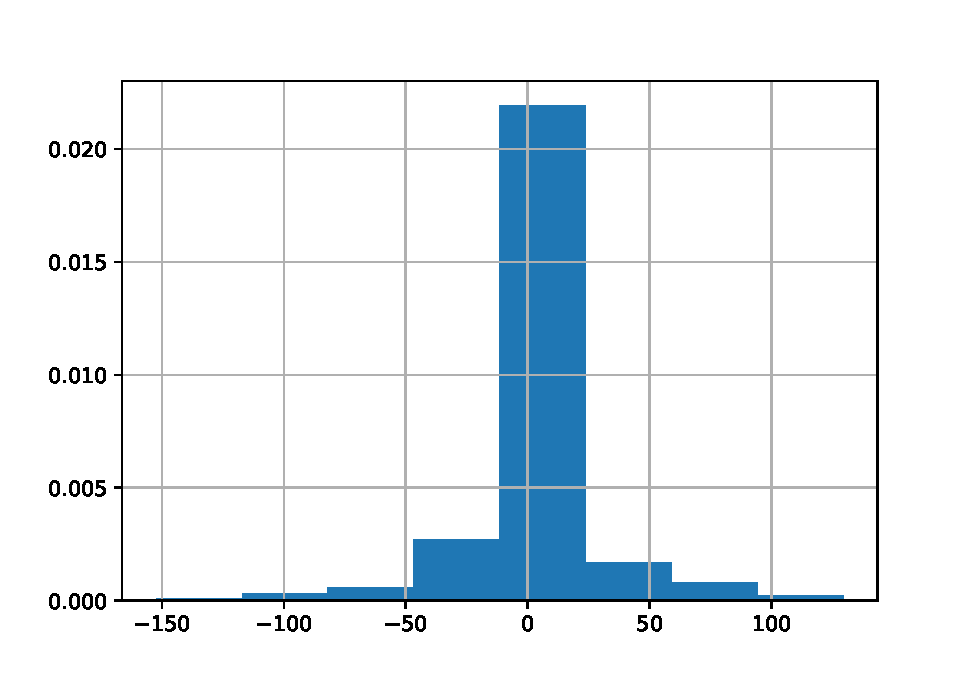
\includegraphics{_main_files/figure-latex/unnamed-chunk-159-35.pdf}

Meg is van a csodaszépen szimmetrikus eloszlást mutató hisztogramunk.
Ezen a ``\emph{relatív gyakoriságos}'' hisztogramon azt a gondolatot kell most elképzelni, hogy milyen alakzatot kapunk, ha \textbf{az oszlopokat összekötjük egy folytonos vonallal}.
Nos, nem kell sokat fantáziálni, a vonnallal összekötés az \textbf{alábbi alakzathoz hasonló függvényt eredményez}:

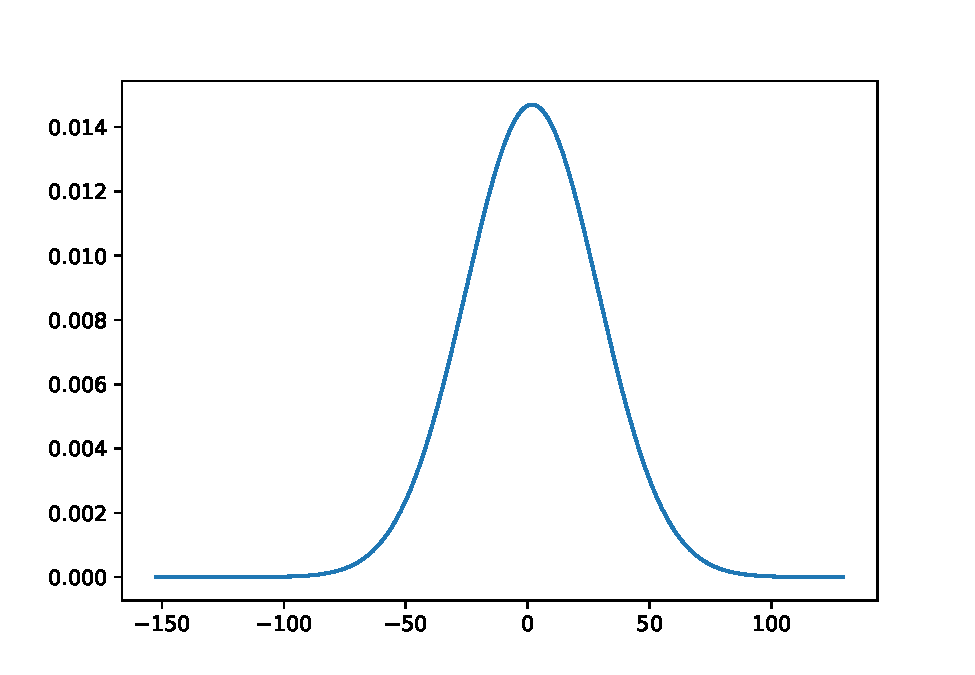
\includegraphics{_main_files/figure-latex/unnamed-chunk-160-37.pdf}

Amit itt látunk az nem más, mint \textbf{egy normális eloszlás sűrűségfüggvénye}. Sőt, pontosítok is, ez \textbf{az alakzat egy \(\mu=1.8\) átlagú és \(\sigma=27.19\) szórású normális eloszlás sűrűségfüggvénye, hiszen ennyi volt a Tesla árfolyamváltozások adatsorának átlaga és szórása, aminek a hisztogramja alapján gondolatban kirajzoltuk ezt a sűrűségfüggvényt}. Ezt ilyenkor úgy szoktuk szakszerűen mondani, hogy amit látunk az egy \(N(1.8,27.19)\) eloszlás sűrűségfüggvénye. Általánosságban egy normális eloszlásra pedig \(N(\mu, \sigma)\) jelöléssel hivatkozunk.

Miért is van ez így? Mivel \textbf{azt, hogy konkrétan milyen egy normális eloszlású sűrűségfüggvény alakja, meghatározza, hogy mennyi az adatsor átlaga és szórása, amire ezt a sűrűségfüggvényt úgymond illeszteni szeretnénk}. Azt, hogy hogyan az alábbi kis interaktív ábra szemlélteti:

Amúgy a normális eloszlás sűrűségfüggvényének hozzárendelési \(f(x)\) utasítása \(\mu\) átlag és \(\sigma\) szórás függvényében az alább alakot ölti.\[f(x)=\frac{1}{\sigma\sqrt{2\pi}}e^{-\frac{1}{2}\left(\frac{x-\mu}{\sigma}\right)^2}\]

Mielőtt szörnyet halunk az Analízis emlékek által kiváltott PTSD-ben, megnyugtatok mindenkit: erre a épletre igazából nekünk nem lesz szükségünk, de egyszer nem árt ha látjuk a függvény mögötti képletet is. :)

\subsection{A sűrűségfüggvény használata}\label{a-sux171rux171suxe9gfuxfcggvuxe9ny-hasznuxe1lata}

No, de ``\emph{Mit adtak nekünk a rómaiak?}'' Azaz jogosan kérdezhetjük, hogy mire tudjuk használni ezt a sűrűségfüggvényt? Első és legfontosabb funkciója, hogy ha a függvény \(f(x)\) formulájába behelyettesítek egy \(x\) értéket, akkor megkapom, hogy \textbf{mi a valószínűsége, hogy az \(Y\) adatsoromból egy véletlenszerűen kihúzott \(Y_i\) érték az \(x\)-et vesz fel}. Magyarul \(f(x)=P(Y_i=x)\).
Most itt egy picit \textbf{pontatlan voltam}. Ugyanis nem egész pontosan a \(Y_i=x\) esemény valószínűségét kapjuk meg, mert nagy értékkészlet esetén az gyakorlatilag \(0\) lenne. Gondoljunk bele: annak a valószínűsége, hogy a Tesla napi árváltozása éppen pont \(2.760009\$\) az tényleg gyakorlatilag \(0\), de a valóságban pont ennyi volt a cucc 2019. május 23-án. Szóval, abszolút nem lehetetlen\ldots{} Azaz, egész pontosan az \(f(x)\) sűrűségfüggvény érték \emph{arányos} a \(P(x<Y_i<x+ \epsilon)\) esemény valószínűségével, ahol az \(\epsilon\) egy \emph{nagyon kicsi} szám. Konkrétan, azt mondhatjuk, hogy \(P(x<Y_i<x+ \epsilon)=f(x) \times \epsilon\). Tehát, annak a valószínűsége, hogy a random módon kihúzott \(Y_i\) értékünk az \(x\)-nek egy \emph{nagyon kicsi}, \(\epsilon\)-nyi környezetébe esik, arányos az \(f(x)\) sűrűségfüggvény értékével. Ha nagyobb ez a valószínűség, akkor nagyobb a sűrűségfüggvény érték is, és fordítva. Szóval, annyi biztosan elmondható, hogy amelyik \(x\) pontnak nagyobb az \(f(x)\) sűrűségfüggvény értéke, annak nagyobb is a bekövetkezési valószínűsége, ha véletlenszerűen kiválasztok egy tetszőleges \(Y_i\) értéket. Csak a két dolog (sűrűségfüggvény és valószínűség) nem ugyan az, az eltérésük egy \(\epsilon\) szorzó.
Emiatt van az is, hogy a Pythonban a \texttt{hist} metódus \texttt{density\ =\ True} beállítással a relatív gyakoriságokat a legnagyobb gyakoriságú \(Y_i\) osztályközép \(\pm 2\) környezet relatív gyakorisága alapján mutatja meg a hisztogram \(y\) tengelyén.
De most nekünk \textbf{szemléletes szempontból teljesen jó lesz, ha úgy gondolunk a helyettesítési értékre \(x\) helyen, mint az \(x\) érték bekövetkezési valószínűsége}. Azaz, mi a \(f(x)=P(Y_i=x)\) értelmezéssel megyünk tovább.

Ez alapján, ha meg akarjuk tudni, hogy mennyi a valószínűsége, hogy a Tesla egy random napi árfolyamváltozása épp a 2019. május 23-i kb. \(2.76\$\)-al lesz egyenlő, akkor ahhoz az alábbi csodát kell kiszámolni.\[P(Y_i=2.76)=f(2.76)=\frac{1}{27.19\sqrt{2\pi}}e^{-\frac{1}{2}\left(\frac{2.76-1.8}{27.19}\right)^2}\]

Hiszen azt tudjuk, hogy a megfigyelt kereskedési napok alapján az árváltozások átlaga \(\mu=1.8\$\) és szórása \(\sigma=27.19\$\).

Na, ezt számolja ki kézzel az, aki papíron tanulja a Stat. II-t. :) Mi Pythonban be tudjuk vetni a \texttt{scipy} csomag \texttt{stats} névterében található függvényeket egy ilyen normális eloszlás sűrűségfüggvény-érték kiszámítására!

Telepítsuk a csomagot és importáljuk a szükséges függvényeket egy \texttt{stats} névtérbe. A \textbf{csomagot nagyon sokat fogjuk hazsnálni a félév során}, és egy szép alapos dokumentációja van. Érdemes olvasgatni! :)

\begin{Shaded}
\begin{Highlighting}[]
\NormalTok{pip install scipy}
\ImportTok{import}\NormalTok{ scipy.stats }\ImportTok{as}\NormalTok{ stats}
\end{Highlighting}
\end{Shaded}

Majd a névtér \texttt{norm.pdf} függvénye segítségével számoljuk ki a keresett valószínűséget! A függvény \textbf{3 paraméterrel operál, ebben a sorrendben: \(x, \mu, \sigma\).} Annyit érdemes megjegyezni, hogy a függvény a \(\mu\) átlagot location-nek, azaz \texttt{loc}-nak, míg a \(\sigma\) szórást \texttt{scale}-nek nevezi a saját kis nyelvjárásában. A függvény neve pedig az angol \emph{probability density function}-ból (valószínűségi sűrűségfüggvény) rövidül \emph{pdf}-nek.

\begin{Shaded}
\begin{Highlighting}[]
\NormalTok{mű }\OperatorTok{=} \FloatTok{1.8}
\NormalTok{szigma }\OperatorTok{=} \FloatTok{27.19}
\NormalTok{stats.norm.pdf(x }\OperatorTok{=} \FloatTok{2.76}\NormalTok{, loc }\OperatorTok{=}\NormalTok{ mű, scale }\OperatorTok{=}\NormalTok{ szigma)}
\end{Highlighting}
\end{Shaded}

\begin{verbatim}
## 0.014663247477553697
\end{verbatim}

Szuper, ez azt jelenti, hogy kb. \(1.466\%\) a valószínűsége annak, hogy egy véletlenszerű napon egy Tesla részvénnyel \(2.76\$\)-t lehet kaszálni.

Ezen a ponton \textbf{érdemes belegondolni, hogyan is reagált a sűrűségfüggvény a szórás növekedésére\ldots ellaposodott!} Na, ez most teljesen érthetővé válik, hiszen \textbf{ha a szórás nő}, az azt jelenti, hogy a \textbf{szélsőségesen magas vagy alacsony \(Y_i\) értékek bekövetkezési valószínűsége is megnő}\ldots és ha a \textbf{függvény \(f(x)\) értéke épp ezekkel a \(P(Y_i=x)\) valószínűségekkel egyenlő}, akkor épp a \textbf{két szélen fog ``meghízni'' a függvény képe}, azaz \textbf{ellaposodik}!

\subsection{A sűrűségfüggvény integrálja}\label{a-sux171rux171suxe9gfuxfcggvuxe9ny-integruxe1lja}

Azért láthatjuk, hogy egy konkrét érték bekövetkezési valószínűsége, alapól nem valami nagy, épp azért, amit fejtegettünk korábban is: az árváltozások értékkészlete elég nagy, egy konkrét érték (vagy annak kis környezetének) bekövetkezési valószínűsége elég kicsi.
Emiatt nem is ezt a kérdést szoktuk általában feltenni a sűrűségfüggvénynek, hanem pl. azt, hogy \textbf{mi a valószínűsége annak, hogy egy véletlenszerűen kihúzott \(Y_i\) érték egy előre megadott \(x\) érték alatt helyezkedik el}? Tehát a \(P(Y_i < x)\) valószínűséget keressük általában.
Ez pedig nem más, mint a \textbf{sűrűségfüggvény \(x\) alatti részének területe}, vagyis a \(\int_{-\infty}^x{f(x)}dx\) improprius integrál.

Na, ha a sűrűségfüggvény helyettesítési értékét nem akartuk kézzel-lábbal kiszámolni, akkor ezt az improprius integrált meg pláne nem!
Szerencsére, \textbf{van erre is beépített függvényünk} a \texttt{scipy} csomagban \texttt{norm.cdf} néven. Ugyan úgy működik, mint a \texttt{norm.pdf}, 3 paramétere van, ugyan abban a sorrendben: \texttt{x,\ loc,\ scale}, csak a \(P(Y_i < x)\)-et számítja ki, nem a \(P(Y_i = x)\)-t a megadott átlagú és szórású normális eloszlás sűrűségfüggvény alapján. A függvény neve az angol \emph{cumulative density function}-ból (kumulált sűrűségfüggvény) rövidül \emph{cdf}-nek. Ha belegondolunk ez logikus, hiszen felösszegezzük (azaz felkumuláljuk) az egyes \(Y_i\) elemek bekövetkezési valószínűségét \(-\infty\)-től \(x\)-ig.

Lássuk akkor hát pl., hogy mennyi a valószínűsége, hogy egy véletlenszerűen kiszúrt kereskedési napon a Teslával \(82\$\)-nál nagyobb \emph{veszteségünk} lesz! Tehát, a \(P(Y_i<-82)\) valószínűséget keressük.

\begin{Shaded}
\begin{Highlighting}[]
\NormalTok{stats.norm.cdf(x }\OperatorTok{=} \OperatorTok{{-}}\DecValTok{82}\NormalTok{, loc }\OperatorTok{=}\NormalTok{ mű, scale }\OperatorTok{=}\NormalTok{ szigma)}
\end{Highlighting}
\end{Shaded}

\begin{verbatim}
## 0.0010280208392538434
\end{verbatim}

Ez pedig a korábban megadott \(\mu\) átlaggal és \(\sigma\) szórással nem más, mint kb. \(0.1\%\). Szóval, szerencsére egy jó kicsi érték! :)

Természetesen ha egy \(x\) érték alá esési valószínűségét ki tudjuk számolni, akkor az \(x\) felé esés valószínűségét már gyerekjáték kiszámolni, hiszen \textbf{a ``felé esés'' az ``alá esés'' komplementer eseménye}, azaz \(P(Y_i>x)=1-P(Y_i<x)\). Szemléletesen pedig itt a \textbf{sűrűségfüggvény \(x\) feletti részének területét} számoljuk ki.

Eszerint gyorsan meg tudjuk adni, hogy mi annak a valószínűsége, hogy egy random napon a Tesla részvényen \(20\$\)-nál többet kaszálunk, hiszen \(P(Y_i>20)=1-P(Y_i<20)\). Tehát, az egész dolog ismét megoldható a \texttt{norm.cdf} függvény segítségével.

\begin{Shaded}
\begin{Highlighting}[]
\DecValTok{1} \OperatorTok{{-}}\NormalTok{ stats.norm.cdf(x }\OperatorTok{=} \DecValTok{20}\NormalTok{, loc }\OperatorTok{=}\NormalTok{ mű, scale }\OperatorTok{=}\NormalTok{ szigma)}
\end{Highlighting}
\end{Shaded}

\begin{verbatim}
## 0.25163173906817715
\end{verbatim}

Na, ez nem is rossz, a \(20\$\) feletti nyereség valószínűsége egy napon egy kicsit több, mint \(25\%\)!

Ha pedig azt szeretnénk megtudni, hogy mi a valószínűsége, hogy a véletlenszerűen kihúzott \(Y_i\) értékünk épp két előre megadott \(x\) és \(y\) érték közé esik, akkor egyszerűen a \textbf{nagyobb érték alá esés valószínűségéből kivonjuk a kisebb érték alá esés valószínűségét}. Azaz, ha \(x>y\), akkor \(P(y<Y_i<x)=P(Y_i<x)-P(Y_i<y)\), de ha \(x<y\), akkor \(P(x<Y_i<y)=P(Y_i<y)-P(Y_i<x)\) a számítás menete.Tehát, ekkor is az egész sztori megoldható pitonban a \texttt{norm.cdf} függvénnyel. Grafikusan pedig úgy képzeljük el a dolgot, mint a \textbf{sűrűségfüggvény \(x\) és \(y\) közötti részének területe}.

Szóval, ha azt szeretném megtudni, hogy mi a valószínűsége annak, hogy egy véletlenszerűen kiválasztott napon egy Tesla részvénnyel \(47\$\) és \(82\$\) közti veszteséget produkálunk, akkor megnézem a \(-47\) alá esés valószínűségét, és kivonom belőle a \(-82\) alá esés valószínűségét (tartom a nagyobból vonom a kisebbet elvet ugyebár).

\begin{Shaded}
\begin{Highlighting}[]
\NormalTok{stats.norm.cdf(x }\OperatorTok{=} \OperatorTok{{-}}\DecValTok{47}\NormalTok{, loc }\OperatorTok{=}\NormalTok{ mű, scale }\OperatorTok{=}\NormalTok{ szigma) }\OperatorTok{{-}}\NormalTok{ stats.norm.cdf(x }\OperatorTok{=} \OperatorTok{{-}}\DecValTok{82}\NormalTok{, loc }\OperatorTok{=}\NormalTok{ mű, scale }\OperatorTok{=}\NormalTok{ szigma)}
\end{Highlighting}
\end{Shaded}

\begin{verbatim}
## 0.035316558328262415
\end{verbatim}

Nagyon jó, akkor már azt is tudjuk, hogy kb. \(3.5\%\) a valószínűsége, hogy a Tesla egy napon \(47\$\) és \(82\$\) közti veszteséget produkál.

\textbf{Összefogalva} tehát a sűrűségfüggvény, \(f(x)\) segítségével a következő események bekövetkezési valószínűsége számítható ki, ahol \(Y_i\) a vizsgált adatsornak egy véletlenszerűen kihúzott \(i\)-edik eleme, \(x\) és \(y\) pedig előre adott számok:

\begin{itemize}
\tightlist
\item
  \(x\) bekövetkezése: \(P(Y_i=x)=f(x)\)
\item
  \(x\) alá esés: \(P(Y_i<x)=\int_{-\infty}^x{f(x)}dx\)
\item
  \(x\) felé esés: \(P(Y_i>x)=1-P(Y_i<x)\)
\item
  \(x\) és \(y\) közé esés: \(P(y<Y_i<x)=P(Y_i<x)-P(Y_i<y)\)
\end{itemize}

Mindezen valószínűségek számolása a hozzájuk tartozó sűrűségfüggvény interaktív ábrájával alább tekinthetők át.
Egy \emph{apró megjegyzés}: az alá-felé-közé esési valószínűségeknél azért hagytam el mindenhol a \(=\) jelet, mert a nagy értékkészlét miatt ugyebár egy konkrét érték bekövetkezési valószínűsége nagyon kicsi, így a tartományba esésnél elhanyagolható. \emph{Nem oszt, nem szoroz úgymond}.

\subsection{Valószínűség vs Relatív Gyakoriság}\label{valuxf3szuxednux171suxe9g-vs-relatuxedv-gyakorisuxe1g}

Na jó, már tudjuk akkor használni a normális eloszlás sűrűségfüggvényét. Jó-jó, de \textbf{ennek mi értelme?} Oké, akkor az előbb a sűrűségfüggvénnyel kiszámoltuk, hogy a Tesla részvényekkel a \(47\$\) és \(82\$\) közti veszteség valószínűsége \(3.5\%\).

\begin{Shaded}
\begin{Highlighting}[]
\NormalTok{stats.norm.cdf(x }\OperatorTok{=} \OperatorTok{{-}}\DecValTok{47}\NormalTok{, loc }\OperatorTok{=}\NormalTok{ mű, scale }\OperatorTok{=}\NormalTok{ szigma) }\OperatorTok{{-}}\NormalTok{ stats.norm.cdf(x }\OperatorTok{=} \OperatorTok{{-}}\DecValTok{82}\NormalTok{, loc }\OperatorTok{=}\NormalTok{ mű, scale }\OperatorTok{=}\NormalTok{ szigma)}
\end{Highlighting}
\end{Shaded}

\begin{verbatim}
## 0.035316558328262415
\end{verbatim}

De ez egy olyan dolog, amit az osztályközös \textbf{gyakorisági tábla relatív gyakoriságaiból is tudtunk már, nem?} Hiszen ott megnéztük a \(-82\) és \(-47\) értékek közötti napok számát, mint kedvező esetek, és elosztottuk a teljes \(N=250\) elemszámmal, mint összes eset. Tehát ilyen elven az is, a \(47\$\) és \(82\$\) közti veszteség valószínűsége, nem?

\begin{Shaded}
\begin{Highlighting}[]
\NormalTok{gyaktábla}
\end{Highlighting}
\end{Shaded}

\begin{verbatim}
##     AlsóHatár  FelsőHatár    f_i  RelatívGyak  KumRelatívGyak         Y_i
## 0 -152.359986 -117.136239    1.0        0.004           0.004 -134.748112
## 1 -117.136239  -81.912491    3.0        0.012           0.016  -99.524365
## 2  -81.912491  -46.688744    5.0        0.020           0.036  -64.300618
## 3  -46.688744  -11.464996   24.0        0.096           0.132  -29.076870
## 4  -11.464996   23.758751  193.0        0.772           0.904    6.146877
## 5   23.758751   58.982498   15.0        0.060           0.964   41.370625
## 6   58.982498   94.206246    7.0        0.028           0.992   76.594372
## 7   94.206246  129.429993    2.0        0.008           1.000  111.818119
\end{verbatim}

Na igen ám, de itt ez a relatív gyakoriság \(2.0\%\)!! Na akkor most kinek higgyek? Mi ez a keresett valószínűség? \(3.5\%\) ahogy a sűrűségfüggvény mondja vagy \(2.0\%\), ahogy a relatív gyakorisággal kiszámoltam? Mi a kettő válasz közötti különbség?

Nos, azt kell észrevenni, hogy a \textbf{relatív gyakoriságos \(2.0\%\) kiszámításánál csak a megfigyelt adatokat, azaz a megfigyelst statisztikai MINTÁT vettem csak figyelembe!!} Tehát a \(2.0\%\) esetén a \textbf{pontos értelmezés az, hogy a megfigyelt napjainknak 2\%-a volt olyan, hogy a részvénnyel 47-82 dollárt veszítettünk!!}

Ezzel szemben a \(3.6\%\), amit az adatokra illeszkedő átlagú és szórású normális eloszlás sűrűségfüggvénye (Gauss görbéje) alapján számoltunk már egy \emph{elvi valószínűség}! Konkréten, \textbf{annak az ELVI valószínűsége, hogy a részvénnyel 47-82 dollár közti összeget veszítek \(3.6\%\)!!} Ez azért lehet egy elvi érték, hiszen mivel az \(x\) tengely felett egy folytonos vonallal összekötött \(f(x)\) függvényről beszélünk, ami így \textbf{pozitív bekövetkezési valószínűséget rendel olyan \(x\) értékekhez is, amik a megfigyelt adatok között még nem szerepelnek!!} Tehát, \textbf{a sűrűségfüggvény megfigyelt adataimon kívüli világot is figyelembe veszi!} Emiatt mondhatom a sűrűségfüggvényből származó értékeket \emph{valódi VALÓSZÍNŰSÉG}nek, és nem csak relatív gyakoriságnak!

\emph{Nota bene}: ehhez azért az is kell, hogy az eloszlás, aminek a sűrűségfüggvényét használom tényleg illeszkedjen az adatokra! Itt azért most a normális eloszlással lehetnek gondok, hiszen amint láttuk pl. az \(\alpha_4\) a Tesla részvények eloszlása kicsit csúcsosabb az \(N(1.8,27.19)\) eloszlás sűrűségfüggvényénél.

Azt, hogy egy eloszlás sűrűségfüggvény mennyire illeszkedik a megfigyelt adatok hisztogramjára a következőképpen tudjuk grafikusan megvizsgálni.

\begin{itemize}
\tightlist
\item
  Először elkészítjük a hisztogramot a \texttt{hist} metódussal, \texttt{density\ =\ True} paraméterrel, hogy az \(y\) tengely skálázása összemérhető legyen a sűrűségfüggvény \(y\) tengelyével, ami ugyebár valószínűségeket mutat ki.
\item
  Utána megadjuk egy külön objektumban a sűrűségfüggvény \(x\) tengelyének tartományát a \texttt{np.arange} függvénnyel. A függvény paraméterezése azt mondja nekünk el, hogy a létrehozott \(x\) tengely a megfigyelt Tesla árváltozások minimuma és maximuma között fog terjedni \(0.01\)-es lépésközzel.
\item
  Kövi lépésben megadjuk a sűrűségfüggvény \(y\) tengelyét egy külön objektumban a \texttt{scipy} csomag \texttt{norm.pdf} függvényével. Ha ennek a függvénynek az \texttt{x} paraméterében több értéket adunk át, akkor mindegyikhez szépen kiszámolja a sűrűségfüggvény \(f(x)\) helyettesítési értékét. Az átlagot (\texttt{loc} paraméter) és szórást (\texttt{scale} paraméter) most közvetlenül a data frame-ből számolom ki a függvényen belül.
\item
  Egy sima \texttt{matplotlib} csomag \texttt{plt} névteréből származó \texttt{plot} függvénnyel felrajzolunk egy olyan vonaldiagramot a hisztogramra, aminek az \(x\) és \(y\) tengelye az előző két pontban létrehozott értékekből áll.
\item
  Végül a \texttt{plt.show()} paranccsal kikényszerítjük, hogy ezt a többrétegű árát így egyben mutassa meg nekünk a gépállat.
\item
  \textbf{FONTOS!} Az alábbi kódsort mindig egyben futtassuk le, mert csak így fogja szépen egyben összerakni a kívánt ábrát! Ha soronként futtatjuk, akkor két külön ábránk lesz belőle!
\end{itemize}

\begin{Shaded}
\begin{Highlighting}[]
\NormalTok{Tesla.TESLA.hist(bins }\OperatorTok{=} \DecValTok{8}\NormalTok{, density }\OperatorTok{=} \VariableTok{True}\NormalTok{)}
\NormalTok{x\_tengely }\OperatorTok{=}\NormalTok{ np.arange(np.}\BuiltInTok{min}\NormalTok{(Tesla.TESLA), np.}\BuiltInTok{max}\NormalTok{(Tesla.TESLA), }\FloatTok{0.01}\NormalTok{)}
\NormalTok{y\_tengely }\OperatorTok{=}\NormalTok{ stats.norm.pdf(x }\OperatorTok{=}\NormalTok{ x\_tengely, loc }\OperatorTok{=}\NormalTok{ np.mean(Tesla.TESLA), scale }\OperatorTok{=}\NormalTok{ np.std(Tesla.TESLA))}
\NormalTok{plt.plot(x\_tengely, y\_tengely)}
\NormalTok{plt.show()}
\end{Highlighting}
\end{Shaded}

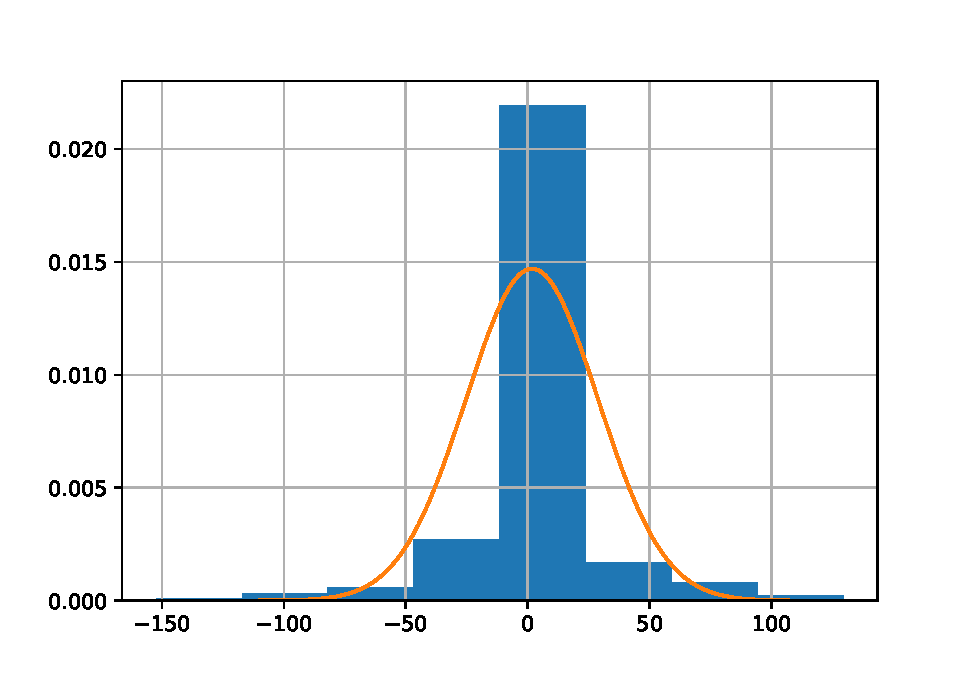
\includegraphics{_main_files/figure-latex/unnamed-chunk-170-1.pdf}

Egyszerűen \emph{utsukushii}, nemigaz? :) Szépen látszik, hogy a valódi árváltozás eloszlás kissé csúcsosabb, mint amit az adatokra illeszkedő normális eloszlás sűrűségfüggvénye sugall.

Egyébként majd ilyen elvi sűrűségfüggvények illeszkedési jóságát valós hisztogramokhoz egzaktabban is megtanuljuk majd mérni a félév során, mint a szemmelverés. :)

\subsection{Centrális Határeloszlás Tétel (CHT)}\label{centruxe1lis-hatuxe1reloszluxe1s-tuxe9tel-cht}

A normális eloszlás esetében viszont van egy \textbf{valószínűségszmítási tétel, ami megadja, hogy a normális eloszlás milyen tulajdonságú adatsorok esetén} lesz egy \textbf{jól illeszkedő eloszlás} a megfigyelt adatok hisztogramjára. Ez a tétel pedig a \textbf{Centrális Határeloszlás Tétel}, leánykori nevén \textbf{CHT}.
Maga a tétel azt mondja, hogy \textbf{ha az adatsor egy \(Y_i\) értéke véletlen hatások összegződéseként áll elő, akkor az adatok hisztogramja normális eloszlású sűrűségfüggvényt követ}.

A tétel tehát ilyen klasszikus \textbf{ha --\textgreater{} akkor} típusú matematiaki tétel. És az \textbf{``akkor'' utáni rész az érthetőbb}. Ha valami felétel teljesül, akkor az adatsorunk normális eloszlású. Ezt oké, értjük. De \textbf{mit jelent az a rész, ami a tétel feltételében van?} Hogy ha \textbf{az \(Y_i\) értékek véletlen hatások összegeként állnak elő}.

Nos, ez \textbf{utóbbi rész megértéséhez nézzünk rá ismét a Tesla árváltozások adatsorának első 5 elemére} a data frame \texttt{head} metódusával.

\begin{Shaded}
\begin{Highlighting}[]
\NormalTok{Tesla.head()}
\end{Highlighting}
\end{Shaded}

\begin{verbatim}
##        Dátum      TESLA
## 0 2019-05-07  -8.279998
## 1 2019-05-08  -2.220002
## 2 2019-05-09  -2.860000
## 3 2019-05-10  -2.459992
## 4 2019-05-13 -12.510009
\end{verbatim}

Vegyük például a 2019 május 13-i \(Y_5=-12.510009\$\)-os veszteséget. Nos \textbf{ez az érték úgy jött ki}, hogy \textbf{az adott nap} (2019. 05. 13.) \textbf{véletlenszerű gazdasági eseményeinek hatása összegződött}, és \textbf{így kötöttünk ki ott, hogy a Tesla részvény a nap végére kb. 12 és fél dollárral kevesebbet ér}. Tehát, reggel mondjuk bejelentik a kínaiak, hogy vizsgálatot indítanak az egyik Tesla gyár munkakörülményei ellen, aminek hatására elkezd esni a részvény értéke, de aztán délben Musk tweetel egyet, hogy ``no para, átviszem a gyárat Mexikóba'', aminek hatására nyugi lesz és elindul felfelé a részvény értéke, de aztán nap végére beesik egy hír, hogy a Mexikóban máris tümtikéznek a tervezett Tesla gyár ellen, ami megint elkezdi levinni a részvény értékét és a nap végére uda jutunk, hogy a részvény \(-12.510009\$\)-al zár\ldots{}
Szóval az \textbf{adott nap véletlenszerű gazdasági eseményeinek összegződéseként áll elő a nap végi \(Y_i\) Tesla árváltozás}. Ezt jelenti az, hogy \textbf{az \(Y_i\) értékek véletlen hatások összegeként állnak elő}. És \textbf{ilyen esetekben az \(Y_i\) adatsorhoz tartozó hisztogram normális eloszlású sűrűségfüggvényt követ a CHT szerint!}

Láthatjuk a \textbf{Tesla részvény vizsgálatának korábbi tapasztalataink alapján}, hogy a csúcsosság miatt azért \textbf{a pénzügyi piacokon ez a tétel nem érvényesül annyira pontosan}, de \textbf{közelítőleg} igen. De \textbf{több egyéb esetben elég szépen érvényesül}: Pl. egy termelőgép által a nap végén gyártott selejtes termékek száma esetén. Az adott napi selejtszám értéke (ha nincs szabotőr a gyárban) az adott napi véletlen hatások összegződése állítja elő. Így, ha több nap nap végi selejtszámait vizsgáljuk, akkor azok hisztogramja csudiszép normális eloszlást kell, hogy kirajzoljon.

\subsection{Inverz Értékek}\label{inverz-uxe9rtuxe9kek}

A sűrűségfüggvényektől lehet ``\emph{visszafelé is kérdezni}''. Tehát, nem csak arra képesek, hogy mondok egy eseményt (pl. mi a valószínűsége, hogy \(80\$\)-nál nagyobb veszteségem lesz a Teslán) és adnak hozzá valószínűséget, hanem arra is, hogy mondok nekik valószínűséget, és az \textbf{inverz értékeik} segítségével adnak hozzá értéket. Szóval, tudok tőlük olyat kérdezni, hogy pl. \emph{Mi az az érték, aminél csak \(5\%\) valószínűséggel veszítek többet a Teslán?}
Magyarul, a \(P(Y_i < x) = 0.05\) kifejezésben megadja nekem a sűrűségfüggvény inverz értéke az \(x\)-et. Ilyenkor az történik a háttérben, hogy a sűrűségfüggvény primitívfüggvényéből (amit hívnak eloszlásfüggvénynek is, de a mi szempontunkból ez az elnevezés nem fontos) ``\emph{kifejezzük az \(x\)-et}''.

Természetesen, a \texttt{scipy}-nak erre is van beépített függvénye \texttt{norm.ppf} néven, ami 3 paramétert kíván: a \(P(Y_i < x)\) alá esési valószínűséget (ezt a függvény \texttt{q}-nak hívja az angol kvantilis=quantile szóból), a \(\mu\) átlagot (\texttt{loc}) és a \(\sigma\) szórást (\texttt{scale}).
Akkor hát lássuk mi is az az érték, aminél csak \(5\%\) valószínűséggel veszítek többet a Teslán?

\begin{Shaded}
\begin{Highlighting}[]
\NormalTok{stats.norm.ppf(q }\OperatorTok{=} \FloatTok{0.05}\NormalTok{, loc }\OperatorTok{=}\NormalTok{ np.mean(Tesla.TESLA), scale }\OperatorTok{=}\NormalTok{ np.std(Tesla.TESLA))}
\end{Highlighting}
\end{Shaded}

\begin{verbatim}
## -42.85439941594264
\end{verbatim}

Oké, tehát csak \(5\%\) valószínűséggel veszítünk kb. \(42.85\$\)-nál többet. Vagy másképp: \(5\%\) a valószínűsége, hogy egy random napon a Tesla árváltozás kisebb lesz, mint \(-42.85\$\). Jó tudni. :) Amúgy pénzügyekben ezeket az értékeket \emph{5\%-os Value at Risk}-nek szokás becézni, mint 5\%-os kockáztatott érték. Általában úgy szól a törvényi szabályozás ezeket az értékeket a befektetési bankoknak be kell raknia biztonsági tartalékba egy-egy pénzügyi befektetési portfólió után.

Ha valaki mélyebben belegondol a Stat. I-es rémképeibe, az \textbf{eloszlások inverz értékeihez is találhat analógiát, mégpedig a percentiliseket!} Hiszen a megfigyelt árváltozások \textbf{5. percentilis}e megadja, hogy mi az az érték, aminél az adatok \(5\%\)-a kisebb csak. Tehát ez az értelmezés lehet a ``\emph{Mi az az érték, aminél csak \(5\%\) a valószínűsége, hogy egy random napon a Tesla árváltozás kisebb lesz?}'' c.~kérdés analógiája.

Lássuk, akkor mi a megfigyelt érváltozások 5. percentilise! Itt most a data frame \texttt{quantile} metódusát vetjük be, aminek a paraméterében tizedestörtként kell megadni a keresett percentilis sorszámát. Tehát az 5. percentilisnél \(0.05\)-öt adunk meg.

\begin{Shaded}
\begin{Highlighting}[]
\NormalTok{Tesla.TESLA.quantile(}\FloatTok{0.05}\NormalTok{)}
\end{Highlighting}
\end{Shaded}

\begin{verbatim}
## -28.48700139999998
\end{verbatim}

Ahha, ez csak kb. \(-28.5\$\)! Tehát a megfigyelt napjaink \(5\%\)-ban volt nagyobb veszteségünk, mint \(28.5\$\)! Ez azért \textbf{lényegesen kisebb érték, mint a sűrűségfüggvényből származó \(42.85\$\)-os veszteség!} És valószínűleg a \textbf{sűrűségfüggvény}ből származó éték a reálisabb, hiszen az a számolás során ugyebár \textbf{olyan értékeket is figyelembe vett} valami pozitív bekövetkezési valószínűséggel, \textbf{amiket a megfigyelt adatsor még egyáltalán ``nem is látott''}, mert kisebbek pl. mint a minimum értéke.
Tehát, megint elmondhatjuk, hogy \textbf{ha az elvi eloszlásból ``keresek percentilist'', akkor a megfigyelt adatokon kívüli világot is figyelembe veszem!} Azaz, \textbf{általánosítok}.

Az tehát, hogy mondjuk egy befektetési bank a befketetéseinek \emph{Value at Risk} értékét a megfigyelt korábbi adatokból, vagy egy azokra jól illeszkedő elvi eloszlásból számolja egyáltalán nem mindegy! Persze itt a jól illeszkedő eloszlás nem feltétlenül a normális eloszlás, de rengeteg egyéb, kellően egzotikus sűrűségfüggvénnyel rendelkező eloszlás van a palettán, lehet válogatni. :)
Persze a válogatáshoz dolgozni is kéne, és nagy a csábítás, hogy egyszerűen inkább a megfigyelt múltbeli adatok alapján mondjon az ember egy percentilist\ldots a nagy befektetési bankok többsége 2008 előtt ezt is csinálta, mert megtehette. Aztán a 2008-as pénzügyi válság lett belőle. Erről is szól részben a The Black Swan: The Impact of the Highly Improbable c.~könyv. Ajánlom minden érdeklődőnek, tartalmas és közérthető olvasmány. :)
2008 óta a törvényi szabályozás (Európában a Bázel III., 2023-tól Bázel IV.) kötelezi a bankokat, hogy a befektetéseikhez Value at Risk-et az adataikra megfelelően illeszkedő elvi eloszlásból számoljanak.

Természetesen ilyen inverz érték formájában ``pozitív'' dolgot is kérdezhetek: \textbf{Mi az az érték, aminél csak \(1\%\) a valószínűsége, hogy többet nyerünk egy Tesla részvényen?} Azaz, mi a \(99\%\)-os valószínűséggel elérhető legnagyobb nyereség?

Ekkor a kérdés ugyebár úgy szól matematikai formájában, hogy mi az az \(x\), aminél \(P(Y_i>x)=0.01\)-et kapunk. De mivel a \texttt{scipy} csomag \texttt{norm.ppf} függvénye \textbf{csak alá esési valószínűséghez tud visszakeresni értékeket}, így inkább a kérdés átfogalmazott verzióját kérdezzük meg a gépszellemtől: \textbf{Mi az az \(x\), aminél \(P(Y_i<x)=0.99\)-et kapunk?}

\begin{Shaded}
\begin{Highlighting}[]
\NormalTok{stats.norm.ppf(q }\OperatorTok{=} \FloatTok{0.99}\NormalTok{, loc }\OperatorTok{=}\NormalTok{ np.mean(Tesla.TESLA), scale }\OperatorTok{=}\NormalTok{ np.std(Tesla.TESLA))}
\end{Highlighting}
\end{Shaded}

\begin{verbatim}
## 64.91674710828752
\end{verbatim}

Tehát, csak \(1\%\) eséllyel tudok többet nyerni egy nap a Teslán, mint kb. \(65\$\).

\subsection{A Standard Normális Eloszlás}\label{a-standard-normuxe1lis-eloszluxe1s}

Még egy fontos dologról kell megemlékeznünk a normális eloszlás kapcsán, a \(\mu=0\) átlagú és \(\sigma=1\) szórású \(N(0,1)\) eloszlásról, ami \textbf{standard normális eloszlás} néven külön helyet kapott a pokolban.

Ami miatt külön kiemelt helye van ennek a standard normális eloszlásnak az az, hogy minden \(N(\mu,\sigma)\) normális eloszlás áttranszformálható strandard normális \(N(0,1)\) eloszlássá. Mégpedig a következő formulával. \[z_i=\frac{Y_i-\mu}{\sigma}\]

Tehát, ha egy \textbf{normális eloszlású \(Y_i\) adatsor minden eleméből kivonom az átlagot és az eredményt elosztom a szórással, akkor az így előálló \(z_i\) adatsor már standard normális eloszlású lesz}. Ez a művelet a \textbf{standardizálás/noralizálás művelet}e.

Amúgy azt, hogy egy adatsor/sokaság valamilyen eloszlást követ, azt \(\sim\) jellel szokás jelölni. Tehát azt mondhatom, hogy \(Y_i \sim N(\mu,\sigma)\), de \(z_i \sim N(0,1)\).

Lássuk is akkor a standardizálást a gyakorlatban a Tesla részvények árváltozásain, és állítsuk elő ezt a \(z_i\) oszlopot.

\begin{Shaded}
\begin{Highlighting}[]
\NormalTok{Tesla[}\StringTok{\textquotesingle{}z\_i\textquotesingle{}}\NormalTok{] }\OperatorTok{=}\NormalTok{ (Tesla.TESLA }\OperatorTok{{-}}\NormalTok{ np.mean(Tesla.TESLA))}\OperatorTok{/}\NormalTok{np.std(Tesla.TESLA)}
\BuiltInTok{round}\NormalTok{(Tesla.describe(), }\DecValTok{2}\NormalTok{) }\CommentTok{\# 2 tizedesre kereítés az átláthatóság miatt}
\end{Highlighting}
\end{Shaded}

\begin{verbatim}
##                             Dátum   TESLA     z_i
## count                         250  250.00  250.00
## mean   2019-11-02 15:56:09.600000    1.78    0.00
## min           2019-05-07 00:00:00 -152.36   -5.68
## 25%           2019-08-05 06:00:00   -3.77   -0.20
## 50%           2019-10-31 12:00:00    1.42   -0.01
## 75%           2020-02-02 06:00:00    6.96    0.19
## max           2020-05-01 00:00:00  129.43    4.70
## std                           NaN   27.19    1.00
\end{verbatim}

Láthatjuk a leíró statisztikákból, hogy a \(z_i\) adatsornak már kb. \(0\) az átlaga és kb. \(1\) a szórása 2 tizedesre kerekítve.

De a hisztogram alapján az eloszlás továbbra is normális maradt.

\begin{Shaded}
\begin{Highlighting}[]
\NormalTok{Tesla.z\_i.hist(bins}\OperatorTok{=}\DecValTok{8}\NormalTok{)}
\end{Highlighting}
\end{Shaded}

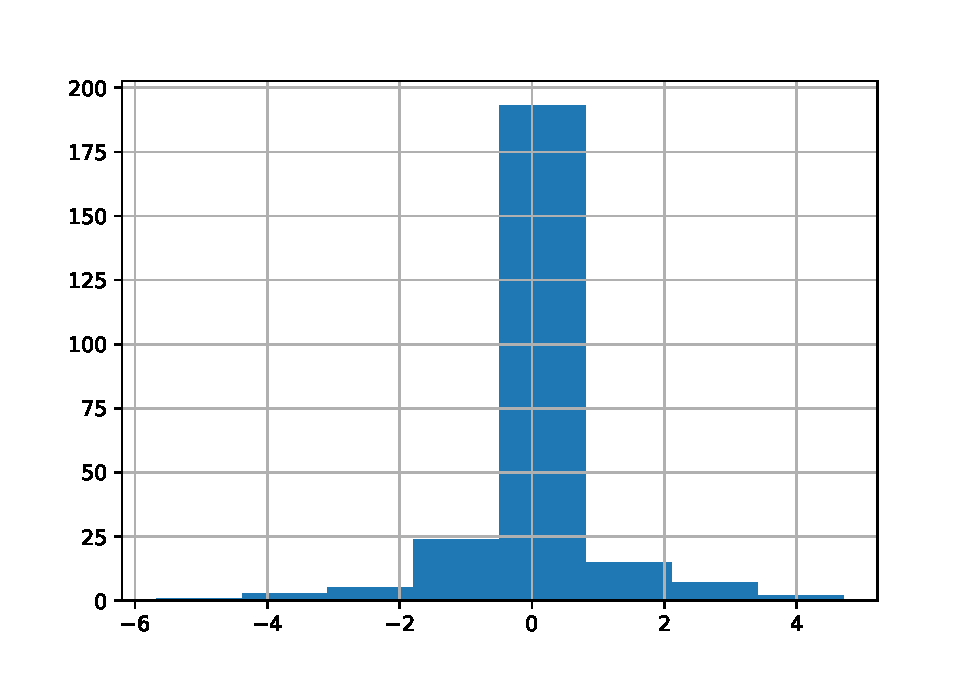
\includegraphics{_main_files/figure-latex/unnamed-chunk-176-3.pdf}

Ami miatt szeretni szokás a standard normális eloszlást az az a jellemzője, hogy

\begin{itemize}
\tightlist
\item
  Az adatok kb. középső \(68.2\%\)-a \(-1\) és \(+1\) között
\item
  Az adatok kb. középső \(95.4\%\)-a \(-2\) és \(+2\) között
\item
  Az adatok kb. középső \(99.7\%\)-a \(-3\) és \(+3\) között
\end{itemize}

helyezkedik el.

Ezt szemlélteti az alábbi ábra is.

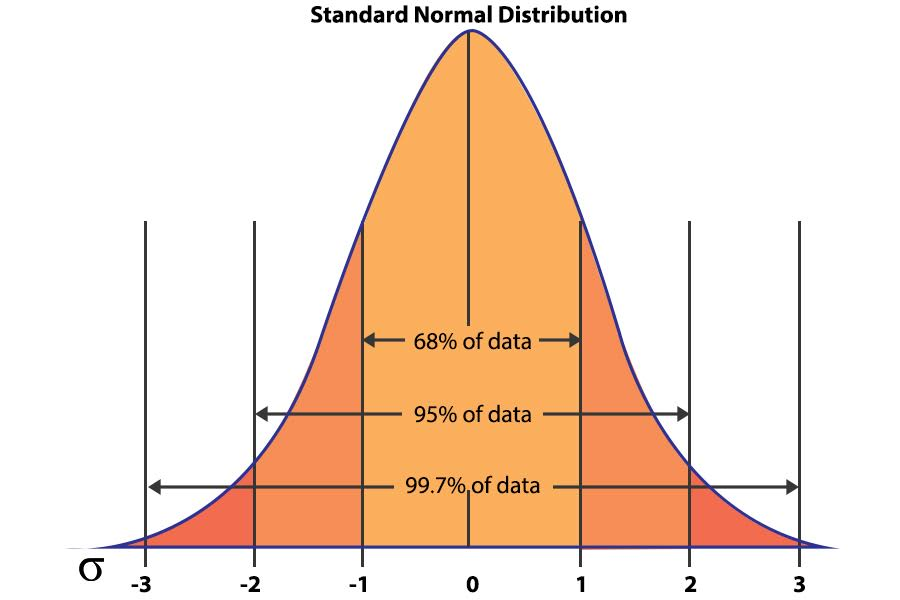
\includegraphics[width=0.5\textwidth,height=\textheight]{stnormal.png}

De ezt ellenőrizhetjük is könnyen Pythonban is, pl. a \(\pm2\)-re. A \texttt{norm.cdf} függvény ugyanis \texttt{loc=0} és \texttt{scale=1} beállításokkal fut, ha nem adunk meg neki mást. Tehát szűmoljuk ki \(z_i \sim N(0,1)\) esetén a \(P(-2 < z_i < +2)\) valószínűséget!

\begin{Shaded}
\begin{Highlighting}[]
\NormalTok{stats.norm.cdf(}\DecValTok{2}\NormalTok{)}\OperatorTok{{-}}\NormalTok{stats.norm.cdf(}\OperatorTok{{-}}\DecValTok{2}\NormalTok{)}
\end{Highlighting}
\end{Shaded}

\begin{verbatim}
## 0.9544997361036416
\end{verbatim}

Jé, ténlyeg kb. \(95.4\%\)! :) \textbf{Ezt a tulajdonságát majd ki fogjuk a későbbiekben használni a standard normális eloszlásnak, szóval jól jegyezzétek meg!} :)

A fenti tulajdonságok miatt sokan szokták úgy keresni a kilógó értékeket egy adatsorban, hogy standardizálják őket, és megnézik melyek azok az értékek, amik kívül esnek a \(\pm2\) intervallumon, mondván az ilyen értékek vagy az adatok alsó vagy a felső \(2.5\%\)-ba tartoznak (a sűrűségfüggvényből látszik, hogy a 95\%-on kívüli 5\% egyeneletesen oszlik meg a függvény két széla között\ldots szimmetriksu az eloszlás ugyebár :)).

Ezt az elvet mi is könnyen tudjuk alkalmazni:

\begin{Shaded}
\begin{Highlighting}[]
\NormalTok{Tesla[(Tesla.z\_i }\OperatorTok{\textless{}} \OperatorTok{{-}}\DecValTok{2}\NormalTok{) }\OperatorTok{|}\NormalTok{ (Tesla.z\_i }\OperatorTok{\textgreater{}} \DecValTok{2}\NormalTok{)]}
\end{Highlighting}
\end{Shaded}

\begin{verbatim}
##          Dátum       TESLA       z_i
## 185 2020-01-30   59.820008  2.138541
## 187 2020-02-03  129.429993  4.703562
## 188 2020-02-04  107.059998  3.879262
## 189 2020-02-05 -152.359986 -5.679967
## 197 2020-02-18   58.369995  2.085110
## 198 2020-02-19   59.019959  2.109060
## 201 2020-02-24  -67.210022 -2.542321
## 204 2020-02-27  -99.799988 -3.743211
## 206 2020-03-02   75.630005  2.721115
## 211 2020-03-09  -95.479980 -3.584026
## 214 2020-03-12  -73.679992 -2.780729
## 216 2020-03-16 -101.549988 -3.807696
## 218 2020-03-18  -68.980011 -2.607542
## 219 2020-03-19   66.420014  2.381741
## 222 2020-03-24   70.709991  2.539820
## 235 2020-04-13   77.950012  2.806604
## 236 2020-04-14   58.940003  2.106114
## 241 2020-04-21  -59.640014 -2.263378
## 245 2020-04-27   73.599976  2.646312
## 249 2020-05-01  -80.559998 -3.034247
\end{verbatim}

Meg is vannak a kiugróan nagy veszteséget vagy nyereséget szolgáltató napjaink. :)

De \textbf{ezzel a módszerrel vigyázzunk!} A standardizált \(z_i\) értékek alapján történő kilógó érték keresés \textbf{csak akkor működik, ha az eredeti (standardizálás előtti) adatsorunk is már eleve normális eloszlású volt!} Hiszen csak ekkor lesz a transzformált adatsor is szimmetrikus normális eloszlású és lesz igaz rá a \(P(-2 < z_i < +2)=0.954\) összefüggés!
Szóval \textbf{kilógó érték kereséshez inkább használjuk} a tetszőleges eloszlásokon is működőképes \textbf{doboz ábrás módszert}! :)

Még egy utolsó gondolat. A standardizált \(z_i\) értékeknek van egy olyan értelmezése is, hogy megadják, az adott érték a \(\sigma\) szórás hányszorosával tér el a \(\mu\) átlagtól.
Tehát, pl. a fenti szűrésben szereplő 2020 január 30-i \(59.82\$\)-os árváltozás a \(27.19\)-es szórás kb. \(2.14\)-szeresével tér el az \(1.8\$\)-os átlagtól.

\section{Az Exponenciális eloszlás}\label{az-exponenciuxe1lis-eloszluxe1s}

Na, hát akkor most engedjük el egy kicsit a Tesla részvények árváltozásait, és vizsgáljunk meg egy másik adatsort, ami a CancerSurvival.xlsx fájlban lakik. Ebben az adattáblában 58 súlyos fej- és nyakrák páciensről rögzítették, hogy \emph{hány hónapig} maradtak életben kemoterápia után. Az adatok valósak, 1988-ból a forrás ez a tanulmány.

Töltsük is be az adatokat egy \texttt{pandas} data frame-be!

\begin{Shaded}
\begin{Highlighting}[]
\NormalTok{Surv }\OperatorTok{=}\NormalTok{ pd.read\_excel(}\StringTok{"CancerSurvival.xlsx"}\NormalTok{)}

\NormalTok{Surv.info()}
\end{Highlighting}
\end{Shaded}

\begin{verbatim}
## <class 'pandas.core.frame.DataFrame'>
## RangeIndex: 58 entries, 0 to 57
## Data columns (total 2 columns):
##  #   Column     Non-Null Count  Dtype  
## ---  ------     --------------  -----  
##  0   Sorszám    58 non-null     float64
##  1   SurvMonth  58 non-null     float64
## dtypes: float64(2)
## memory usage: 1.0 KB
\end{verbatim}

\begin{Shaded}
\begin{Highlighting}[]
\NormalTok{Surv.head()}
\end{Highlighting}
\end{Shaded}

\begin{verbatim}
##    Sorszám  SurvMonth
## 0      1.0       6.53
## 1      2.0       7.00
## 2      3.0      10.42
## 3      4.0      14.48
## 4      5.0      16.10
\end{verbatim}

Mint láthatjuk, ebben a data frame-ben is csak két oszlopunk van. Az első a páciens sorszáma, a második pedig a kemoterápiától számítot túlélési idő hónapokban megadva (\emph{SurvMonth}).

Nézzünk rá egy hisztogrammal a túlélési idők eloszlására. Mivel most \(N=58\), így a legksiebb olyan \(k\), amire \(2^k\) már épp nagyobb \(N\)-nél az a 6 lesz, hiszen \(2^6=64\). Tehát \(6\) osztályközt hozunk létre a hisztogramon.

\begin{Shaded}
\begin{Highlighting}[]
\NormalTok{Surv.SurvMonth.hist(bins}\OperatorTok{=}\DecValTok{6}\NormalTok{)}
\end{Highlighting}
\end{Shaded}

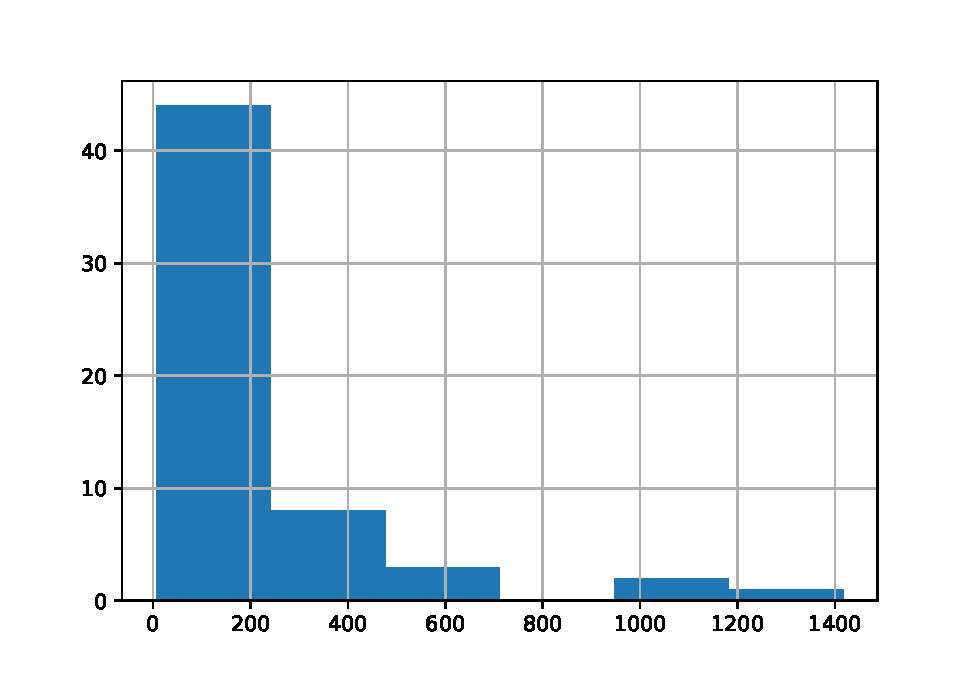
\includegraphics{_main_files/figure-latex/unnamed-chunk-180-5.pdf}

Nos, hát itt az látszódik, hogy az eloszlásunk jobbra elnyúló: a túlélési idők nagy többsége (45 az 58-ból konkrétan) \(256\) hónapon belüli, de a maradék \(13\) meghaladja ezt, sőt \(3\) páciens \(1000\) hónapnál is hosszabb ideig élt túl a kemoterápia után.

A jobbra elnyúlás miatt, ha folytonos vonallal összekötjük a hisztogram oszlopait, akkor valami ilyesmi függvényábrát kapunk, mint alább.

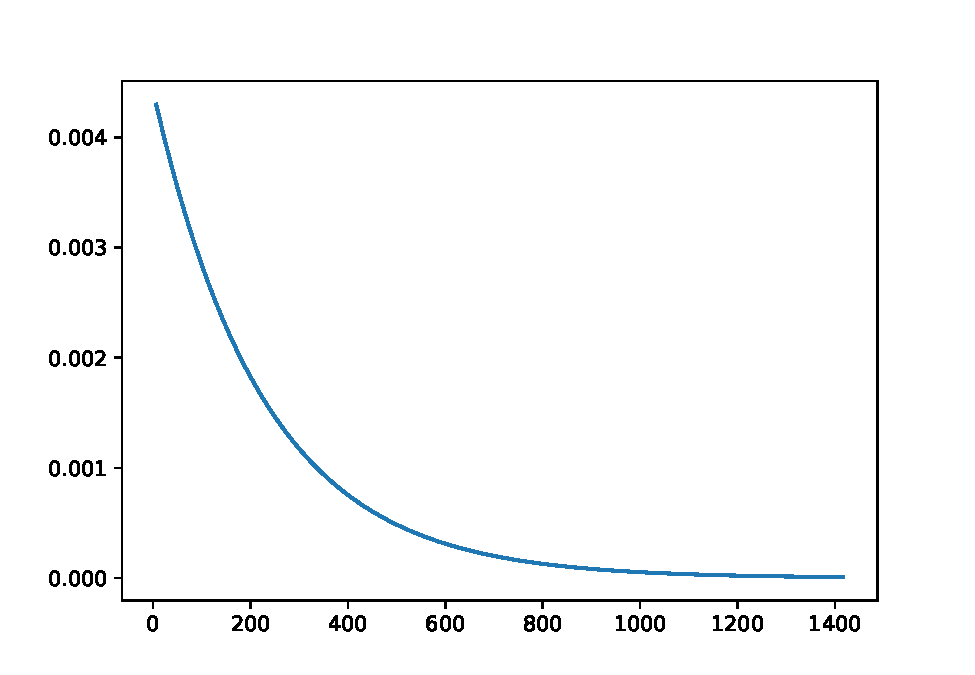
\includegraphics{_main_files/figure-latex/unnamed-chunk-181-7.pdf}

Ez az alakzat pedig az \textbf{exponenciális eloszlás sűrűségfüggvénye}. Ennek a sűrűségfüggvénynek a konkrét alakját egy \(\lambda\) paraméter határozza meg. Minél nagyobb \(\lambda\), annál meredekebben jobbra elnyúló a sűrűségfüggvény. Ezt alább lehet kipróbálni.

Természetesen a \(\lambda\)-nak van köze a valós adatok átlagához és szórásához, egész konkrétan mindkét érték \(\mu=\sigma=\frac{1}{\lambda}\). Tehát, az exponenciális eloszlásban azonos átlagot és szórást tételezünk fel az adatokra, és ennek a közös értéknek a reciproka (a \(\lambda\)) határozza meg, hogy mennyire meredeken nyúlik jobbra az eloszlás sűrűségfüggvénye. Emiatt az exponenciális eloszlásokat \(Exp(\lambda)\) módon szokták jelölni.

Persze valós adatokon gyakorlatilag sosem fog teljesülni, hogy \(\mu=\sigma\), de láthatjuk egy \texttt{describe} metódusból, hogy a túlélési adatok esetén a két mutató értéke aránylag közel esik egymáshoz: \(\mu=226.17 \approx \sigma=273.94\)

\begin{verbatim}
## count      58.000000
## mean      226.173793
## std       273.943381
## min         6.530000
## 25%        83.250000
## 50%       151.500000
## 75%       237.000000
## max      1417.000000
## Name: SurvMonth, dtype: float64
\end{verbatim}

A \texttt{scipy} csomagban a \texttt{norm.pdf}, \texttt{norm.cdf} és \texttt{norm.ppf} függvények mintájára léteznek \texttt{expon.pdf}, \texttt{expon.cdf} és \texttt{expon.ppf} függvények is. Használatuk és jelentésük teljesen megegyezik a normális eloszlásnál látott függvényekkel. Egyetlen különbség ugyebár, hogy exponenciális eloszlásnál csak az egységes \(\lambda\)-t kell megadni a külön \(\mu\) és \(\sigma\) helyett, mint ahogy a normális eloszlásnál működött a dolog.
A \texttt{scipy} csomag ezt úgy oldja meg, hogya a szórásból számolja vissza a \(\lambda\)-t, tehát a függvényeknek a \texttt{scale} paraméterében kell átadni az adatok szórását, amire az exponenciális eloszlást illeszteni akarjuk.
Ez alapján akkor most a túlélési idők esetében \(\lambda=\frac{1}{\sigma}=\frac{1}{273.94}=0.00365\). Tehát az egyes \(Y_i\) túlélési idők \(Exp(0.00365)\) eloszlástkövetnek: \(Y_i \sim Exp(0.00365)\)

Ezek alapján számoljunk ki pár valószínűséget a túlélési időkre vonatkozóan:

\begin{enumerate}
\def\labelenumi{\arabic{enumi}.}
\tightlist
\item
  Mi a valószínűsége, hogy kemoterápia után pont egy évet, azaz \(12\) hónapot fogunk élni?
\end{enumerate}

\begin{Shaded}
\begin{Highlighting}[]
\NormalTok{stats.expon.pdf(}\DecValTok{12}\NormalTok{, scale }\OperatorTok{=}\NormalTok{ np.std(Surv.SurvMonth))}
\end{Highlighting}
\end{Shaded}

\begin{verbatim}
## 0.003523104116060953
\end{verbatim}

Ez egy jó alacsony, kb. \(0.3\%\)-os valószínűség. Nem lepődünk meg, hiszen egy konkrét pont bekövetkezése a nagy túlélési idő-értékkészlet miatt itt is kicsi.

\begin{enumerate}
\def\labelenumi{\arabic{enumi}.}
\setcounter{enumi}{1}
\tightlist
\item
  Mi a valószínűsége, hogy kemoterápia után több, mint öt évet, azaz \(60\) hónapot fogunk élni?
\end{enumerate}

\begin{Shaded}
\begin{Highlighting}[]
\DecValTok{1} \OperatorTok{{-}}\NormalTok{ stats.expon.cdf(}\DecValTok{60}\NormalTok{, scale }\OperatorTok{=}\NormalTok{ np.std(Surv.SurvMonth))}
\end{Highlighting}
\end{Shaded}

\begin{verbatim}
## 0.8017677791228195
\end{verbatim}

Az eredmény kb. \(80\%\), egész jó kilátások!

\begin{enumerate}
\def\labelenumi{\arabic{enumi}.}
\setcounter{enumi}{2}
\tightlist
\item
  Mi a valószínűsége, hogy a kemoterápia utáni harmadik év során, azaz \(24\) és \(36\) hónapközött fogunk elpatkolni?
\end{enumerate}

\begin{Shaded}
\begin{Highlighting}[]
\NormalTok{stats.expon.cdf(}\DecValTok{36}\NormalTok{, scale }\OperatorTok{=}\NormalTok{ np.std(Surv.SurvMonth)) }\OperatorTok{{-}}\NormalTok{ stats.expon.cdf(}\DecValTok{24}\NormalTok{, scale }\OperatorTok{=}\NormalTok{ np.std(Surv.SurvMonth))}
\end{Highlighting}
\end{Shaded}

\begin{verbatim}
## 0.03956914214644276
\end{verbatim}

A számítások alapja itt is az, hogy \(f(x)=P(Y_i=x)\), tehát \textbf{a sűrűségfüggvény helyettesítési értékre \(x\) helyen megegyezik az \(x\) érték bekövetkezési valószínűségével} egy véletlen húzás esetén az adatsorból. A \(P(Y_i<x)\) valószínűség pedig exponenciális sűrűségfüggvény esetén is az \(\int_{-\infty}^x{f(x)}dx\) improprius integrállal számítható, azaz a sűrűségfüggvény \(x\) alatti területével egyezik meg.

Ezeket a vizuális jelentéstartalmakat az alábbi interaktív ábrán meg lehet nézni és ki lehet próbálni úgy, ahogy a normális eloszlásnál lehetett.

Természetesen \emph{inverz értéket} is tudunk számolni az exponenciális eloszlásban is. Nézzük meg pl, hogy Mi az az idő, aminél csak \(1\%\) a valószínűsége, hogy egy kemoterápiával kezelt fej- és nyakrák páciens tovább él.
Ugyebár a számításhoz úgy kell átfogalmazni a kérdést, hogy mi az az idő, ami esetén csak \(99\%\) a valószínűsége, hogy egy kemoterápiával kezelt fej- és nyakrák páciens már \emph{NEM} él tovább. Hiszen az \texttt{expon.ppf} függvény is \emph{alá esési} valószínűségekból dolgozik, mint a \texttt{norm.ppf}.

\begin{Shaded}
\begin{Highlighting}[]
\NormalTok{stats.expon.ppf(}\FloatTok{0.99}\NormalTok{, scale }\OperatorTok{=}\NormalTok{ np.std(Surv.SurvMonth))}
\end{Highlighting}
\end{Shaded}

\begin{verbatim}
## 1250.6331218835987
\end{verbatim}

A megfejtés kb. \(1250\) hónap, azaz \(104\) év! De hát ugye ez a nagy érték alapvetően a jobbra elnyúlás miatt van, hiszen a jobbra elnyúló eloszlásokra jellemzőek a felfelé kilógó értékek, így a jobbra elnyúló sűrűségfüggvényeknek is számolnia kell ezekkel az outlier elemekkel.

Végül pedig nézzük meg szépen, hogy ez az exponenciális sűrűségfüggvény mennyire illeszkedik a túlélési idők hisztogramjára, ahogy a normális eloszlás esetén is megtettük egy hisztogramra illesztett \texttt{matplotlib}-es vonaldiagrammal.

\begin{Shaded}
\begin{Highlighting}[]
\NormalTok{Surv.SurvMonth.hist(bins }\OperatorTok{=} \DecValTok{6}\NormalTok{, density }\OperatorTok{=} \VariableTok{True}\NormalTok{)}
\NormalTok{x\_tengely }\OperatorTok{=}\NormalTok{ np.arange(np.}\BuiltInTok{min}\NormalTok{(Surv.SurvMonth), np.}\BuiltInTok{max}\NormalTok{(Surv.SurvMonth), }\FloatTok{0.01}\NormalTok{)}
\NormalTok{y\_tengely }\OperatorTok{=}\NormalTok{ stats.expon.pdf(x\_tengely, scale }\OperatorTok{=}\NormalTok{ np.mean(Surv.SurvMonth))}
\NormalTok{plt.plot(x\_tengely, y\_tengely)}
\NormalTok{plt.show()}
\end{Highlighting}
\end{Shaded}

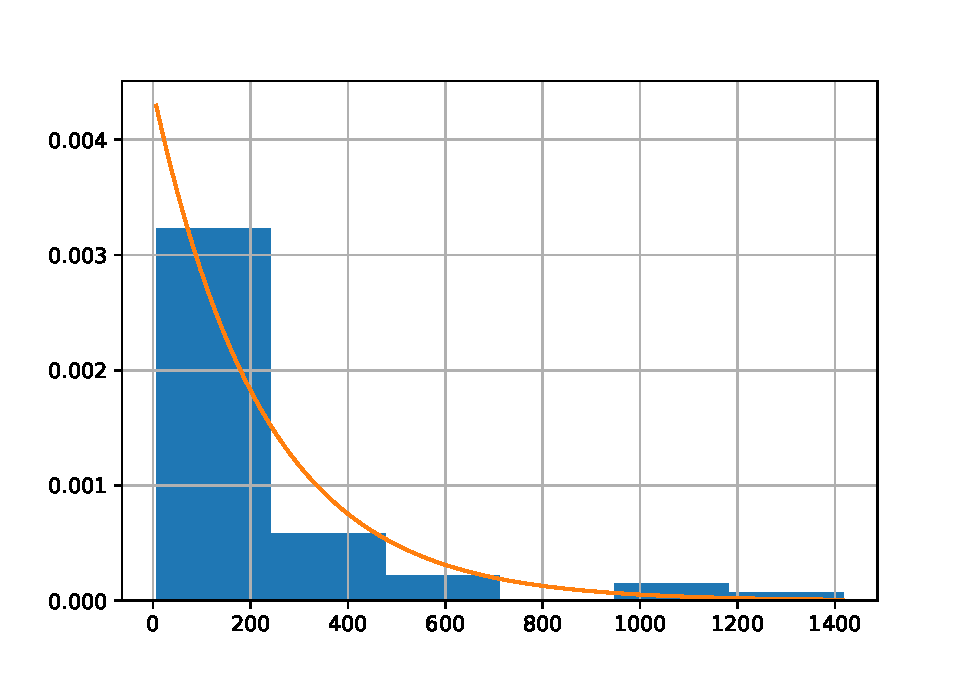
\includegraphics{_main_files/figure-latex/unnamed-chunk-189-1.pdf}

Itt egész pofásnak tűnik az illeszkedés, így szemmelverésre jobban is illeszkedik ez az exponenciális eloszlás a túlélési időkre, mint a normális eloszlás illeszkedett a Tesla árváltozásokra. :)

\section{A Varianciahányados Pythonban - Kokain a Balatonban}\label{a-varianciahuxe1nyados-pythonban---kokain-a-balatonban}

Egy dolgot kellene még átismételnünk a Stat. I-es rémképeink közül, ami többször is elő fog jönni a Stat. II-es tanulmányinkban: a \textbf{Varianciahányados} fogalmát.

A varianciahányados ugyebár arra szolgál, hogy \textbf{két ismérv, egy minőségi (``szöveges'') és egy mennyiségi (``számértékű'') ismérv kapcsolatának szorosságát adja meg, százalékos formában}. Tehát olyan kérdéseket lehet vele megválaszolni, mint\ldots{}

\begin{itemize}
\tightlist
\item
  Hány százalékban befolyásolja a nem (minőségi simérv) a fizetést (mennyiségi ismérv)?
\item
  Hány százalékban befolyásolja a kerület (minőségi simérv) a budapesti lakások árát (mennyiségi ismérv)?
\item
  Hány százalékban befolyásolja a Balaton Sound jelenléte (minőségi simérv) a Balatonban található kokain mennyiségét (mennyiségi ismérv)?
\end{itemize}

A legutolsó kérdés a listán elsőre meredeknek tűnik, de ez a tanulmány épp egy ilyen kérdésekkel is foglalkozik. Az általuk használt adatok egy részét találjuk a BalatonSoundCocaine.xlsx című fájlban.

A fájlban \textbf{3 balatoni vízminőséget ellenőrző állomás összesen \(N=540\) mérését látjuk}. Egy állomás egy hónapban \(20\) mérést végez, és mindhárom állomás esetén a nyári hónapok (június, július, augusztus) mérései vannak a fájlban 3 évre (2017, 2018, 2019). Így egy állomás esetében \(20 \times 3 \times 3 = 180\) mérésünk van, azaz a három állomásra összesen \(3 \times 180 = 540\) mérési adatunk van. Az \textbf{Excel fájlunk mindegyik mérés esetében tartalmazza a mérőállomás sorszámát (1., 2., 3.), a mérés évét és hónappját, valamint a vízben mért kokain mennyiségét nanogram/literben}.

Olvassuk is be az Excelt egy data frame-be és lessük meg, hogy ez tényleg így van-e!

\begin{Shaded}
\begin{Highlighting}[]
\NormalTok{Balcsi }\OperatorTok{=}\NormalTok{ pd.read\_excel(}\StringTok{"BalatonSoundCocaine.xlsx"}\NormalTok{)}

\NormalTok{Balcsi.info()}
\end{Highlighting}
\end{Shaded}

\begin{verbatim}
## <class 'pandas.core.frame.DataFrame'>
## RangeIndex: 540 entries, 0 to 539
## Data columns (total 4 columns):
##  #   Column   Non-Null Count  Dtype  
## ---  ------   --------------  -----  
##  0   Ev       540 non-null    int64  
##  1   Honap    540 non-null    object 
##  2   Allomas  540 non-null    object 
##  3   Kokain   540 non-null    float64
## dtypes: float64(1), int64(1), object(2)
## memory usage: 17.0+ KB
\end{verbatim}

\begin{Shaded}
\begin{Highlighting}[]
\NormalTok{Balcsi.head()}
\end{Highlighting}
\end{Shaded}

\begin{verbatim}
##      Ev   Honap     Allomas   Kokain
## 0  2017  június  1. állomás  0.03891
## 1  2017  június  1. állomás  0.01879
## 2  2017  június  1. állomás  0.03193
## 3  2017  június  1. állomás  0.03510
## 4  2017  június  1. állomás  0.01107
\end{verbatim}

Igen, az oszlopok (ismérvek) neve és adattípusa és az első öt sor tartalma alapján úgy néz ki, hogy rendben van a tábla, azok az oszlopok szerepelnek benne, amit a leírás alapján vártunk is.

Oké, akkor itt mérési adatokat látunk. Hogy a túróba jön az egészhez a Balaton Sound. Egyrészt úgy, hogy a három mérőállomás épp a Sound helyszíne környékén található Siófokon. Konkrét koordináták az alábbi ábrán.

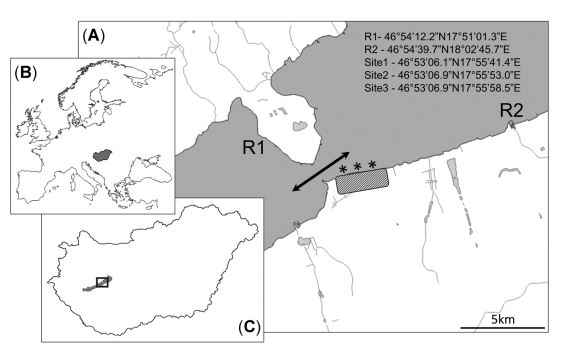
\includegraphics[width=0.5\textwidth,height=\textheight]{balcsi.jpg}

És hát a mérések pont a fesztivál előtt (június), közben (július) és után (augusztus) készültek. Tehát, ha \textbf{a Sound jelenlétének van hatása a víz kokain tartalmára, akkor a mérés hónapja aránylag nagy százalékban kell, hogy meghatározza a kokaintartalmat}. Szóval a vizsgált \textbf{minőségi ismérvünk a mérés hónapja, mennyiségi ismérvünk a kokaintartalom} lesz. A két ismérv kapcsolatának szorosságát pedig akkor a varianciahányados adja meg.

A varianciahányados kiszámításának első lépése egy olyan segétáblázat összeállítása, amely sorait a minőségi ismérv lehetséges értékei adják, és 3 oszlopa van, ami a minőségi ismérv \(j\) indexszel jelölt csoportjai szerint bontva tartalmazza az elemszámokat (\(N_j\)), a mennyiségi ismérv részátlagait (\(\bar{Y}_j\)) és szórásait (\(\sigma_j\)).
Ezt a segédtáblát Pythonban a data frame-k \texttt{groupby} és \texttt{agg} metódusaival hozhatjuk létre. Persze az \texttt{agg}-n belül használjuk a \texttt{numpy} csomag \texttt{mean} és \texttt{std} függvényeit is a \texttt{count} mellett (amely utóbbi függvényt stringként kell beadni az \texttt{agg}-ba, mint az oszlopneveket). Illetve, ne felejtsük el a végén a `reset\_index`` metódus használatát, különben a minőségi ismérvünk értékei a data frame sorindexeiként végzik, és nem lesz külön oszlopuk!

\begin{Shaded}
\begin{Highlighting}[]
\NormalTok{Segéd }\OperatorTok{=}\NormalTok{ Balcsi.groupby(}\StringTok{\textquotesingle{}Honap\textquotesingle{}}\NormalTok{).agg(}
\NormalTok{  Elemszam }\OperatorTok{=}\NormalTok{ (}\StringTok{\textquotesingle{}Kokain\textquotesingle{}}\NormalTok{, }\StringTok{\textquotesingle{}count\textquotesingle{}}\NormalTok{),}
\NormalTok{  Reszatlagok }\OperatorTok{=}\NormalTok{ (}\StringTok{\textquotesingle{}Kokain\textquotesingle{}}\NormalTok{, np.mean),}
\NormalTok{  Szorasok }\OperatorTok{=}\NormalTok{ (}\StringTok{\textquotesingle{}Kokain\textquotesingle{}}\NormalTok{, np.std)}
\NormalTok{).reset\_index()}
\end{Highlighting}
\end{Shaded}

\begin{verbatim}
## <string>:1: FutureWarning: The provided callable <function mean at 0x00000167D93F13A0> is currently using SeriesGroupBy.mean. In a future version of pandas, the provided callable will be used directly. To keep current behavior pass the string "mean" instead.
## <string>:1: FutureWarning: The provided callable <function std at 0x00000167D93F14E0> is currently using SeriesGroupBy.std. In a future version of pandas, the provided callable will be used directly. To keep current behavior pass the string "std" instead.
\end{verbatim}

\begin{Shaded}
\begin{Highlighting}[]
\NormalTok{Segéd}
\end{Highlighting}
\end{Shaded}

\begin{verbatim}
##        Honap  Elemszam  Reszatlagok   Szorasok
## 0  augusztus       180     0.029198   0.011618
## 1     július       180    64.859463  95.853905
## 2     június       180     0.029752   0.011614
\end{verbatim}

Meg is vagyunk! Látszik, hogy \textbf{a Sound hónapjának van hatása}: júliusban nagyságrendekkel több az átlagos kokain mennyisége a Balaton vizének, mint a másik két nyári hónapban. De a \textbf{hatás nagyságát nehéz megfogni már szemmelveréssel}, mivel a \textbf{kokain mennyiségek szórása is ebben a hónapban a legnagyobb}. Sőt, ez az egyetlen hónap, amikor a konkrét mérések kokain mennyiségének szórása \emph{nagyobb} az átlagos kokain mennyiségnél! Szóval, kell azért egy check arra a varianciahányadosra.

A varianciahányados, a \(H^2\) mutató értékéhez úgy jutunk el, hogy \textbf{elkezdjük az előbb felépített segédtáblázatunk alapján kiszámolni a mennyiségi ismérv (azaz most a kokain mennyiség) teljes, hónapoktól független teljes átlagát és teljes szórását}. Ugyebár a \textbf{teljes átlagos kokainmennyiség (főátlag, \(\bar{Y}\)), nem más, mint a részátlagok (\(\bar{Y}_j\)) részelemszámokkal (\(N_j\)) súlyozott átlaga}: \[\bar{Y}=\frac{\sum_j{N_j\bar{Y}_j}}{\sum_j{N_j}}\]

Ilyen stílusú súlyozott átlagokat számolgattunk már az 1.4. fejezetben, csak gyakorisági táblából. Ez ugyan az a szitu, és itt is a \texttt{np.sum} függvényt be tudjuk vetni. Ellenőrzéshez ki tudjuk számolni ezt a főátlagot úgy is, hogy az \texttt{np.mean} függvényt ráeresztjük a data frame teljes \texttt{Kokain} oszlopára.

\begin{Shaded}
\begin{Highlighting}[]
\NormalTok{főátlag }\OperatorTok{=}\NormalTok{ np.}\BuiltInTok{sum}\NormalTok{(Segéd.Elemszam }\OperatorTok{*}\NormalTok{ Segéd.Reszatlagok)}\OperatorTok{/}\NormalTok{(np.}\BuiltInTok{sum}\NormalTok{(Segéd.Elemszam))}
\NormalTok{főátlag}
\end{Highlighting}
\end{Shaded}

\begin{verbatim}
## 21.63947090740741
\end{verbatim}

\begin{Shaded}
\begin{Highlighting}[]
\NormalTok{np.mean(Balcsi.Kokain)}
\end{Highlighting}
\end{Shaded}

\begin{verbatim}
## 21.639470907407407
\end{verbatim}

Stimm egészen az utolsó jó sokadik tizedesjegyig. Ezzel megvagyunk. :)

A variancia-hányados lelke viszont abban leledzik, hogy a kokainmennyiség (mint mennyiségi ismérv) teljes szórása (\(\sigma\)) csak úgy kapható meg a segédtábla alapján, ha előbb kiszámoljuk a belső szórást (\(\sigma_B\)) és a külső szórást (\(\sigma_K\)).

A belső szórást a \textbf{belső variancián, azaz belső szórásnégyzeten keresztül kapjuk meg}. Ez pedig nem más, mint a \textbf{részszórások \(\sigma_j^2\) négyzeteinek elemszámokkal (\(N_j\)) súlyozott átlaga}. \[\sigma_B^2=\frac{\sum_j{N_j\sigma_j^2}}{\sum_j{N_j}}\]

Az előző számítás alapján ez is egész könnyen tud menni Pythonban, csak a részszórások négyzetre emelésére kell figyelni.

\begin{Shaded}
\begin{Highlighting}[]
\NormalTok{belső\_var }\OperatorTok{=}\NormalTok{ np.}\BuiltInTok{sum}\NormalTok{(Segéd.Elemszam }\OperatorTok{*}\NormalTok{ Segéd.Szorasok}\OperatorTok{**}\DecValTok{2}\NormalTok{)}\OperatorTok{/}\NormalTok{(np.}\BuiltInTok{sum}\NormalTok{(Segéd.Elemszam))}
\NormalTok{belső\_var}
\end{Highlighting}
\end{Shaded}

\begin{verbatim}
## 3062.6571029636407
\end{verbatim}

A belső szórás pedig egyszerűen a belső variancia gyöke. \(\sigma_B=\sqrt{\sigma_B^2}\) Általánosságban \(\sigma_B\) azt jelenti, hogy \textbf{egy véletlenszerűen kiválasztott egyed konkrét mennyiségi ismérv értéke várhatóan mennyivel tér el saját csoportjának átlagától}.

Konkrét esetünkben ez az alábbi módon néz ki.

\begin{Shaded}
\begin{Highlighting}[]
\NormalTok{belső\_szórás }\OperatorTok{=}\NormalTok{ np.sqrt(belső\_var)}
\NormalTok{belső\_szórás}
\end{Highlighting}
\end{Shaded}

\begin{verbatim}
## 55.34127847243539
\end{verbatim}

Tehát, \textbf{egy mérés kokainmennyisége várhatóan \(55.3\) nanogram/literrel tér el saját hónapjának átlagos kokainmennyiségtől}. Ami azért nem egy elhanyagolható mennyiségű szóródás a mérési hónapokon \emph{belül}.

A másik vége a dolognak a külső szórás, ami szintén a négyzetén, a külső variancián keresztül számítható. A külső variancia pedig a \textbf{részátlagok \(\bar{Y}_j\) elemszámokkal (\(N_j\)) súlyozott szórása a mennyiségi ismérv főátlaga \(\bar{Y}\) körül}. \[\sigma_K^2=\frac{\sum_j{N_j(\bar{Y}_j-\bar{Y})^2}}{\sum_j{N_j}}\]

Az 1.4. fejezet alapján ezt is meg tudjuk azért alkotni \texttt{np.sum} bevetésével.

\begin{Shaded}
\begin{Highlighting}[]
\NormalTok{külső\_var }\OperatorTok{=}\NormalTok{ np.}\BuiltInTok{sum}\NormalTok{(Segéd.Elemszam }\OperatorTok{*}\NormalTok{ (Segéd.Reszatlagok }\OperatorTok{{-}}\NormalTok{ főátlag)}\OperatorTok{**}\DecValTok{2}\NormalTok{)}\OperatorTok{/}\NormalTok{(np.}\BuiltInTok{sum}\NormalTok{(Segéd.Elemszam))}
\NormalTok{külső\_var}
\end{Highlighting}
\end{Shaded}

\begin{verbatim}
## 933.983870298589
\end{verbatim}

A külső szórás pedig egyszerűen a külső variancia gyöke. \(\sigma_K=\sqrt{\sigma_K^2}\) Általánosságban \(\sigma_K\) azt jelenti, hogy \textbf{egy csoport átlaga várhatóan mennyivel tér el a mennyiségi ismérv főátlagától}.

Konkrét esetünkben ez az alábbi módon néz ki.

\begin{Shaded}
\begin{Highlighting}[]
\NormalTok{külső\_szórás }\OperatorTok{=}\NormalTok{ np.sqrt(külső\_var)}
\NormalTok{külső\_szórás}
\end{Highlighting}
\end{Shaded}

\begin{verbatim}
## 30.561149688756622
\end{verbatim}

Tehát, \textbf{egy hónap átlagos kokainmennyisége várhatóan \(30.5\) nanogram/literrel tér el az átlagosan mért kokainmennyiségétől}. Tehát a hónapok \emph{között} is van egy jelentős szóródásunk, viszont ez kicsit kisebb, mint a csoporton belüli szóródás.

Ebből a két tényezőből pedig összeadható a \textbf{teljes variancia: \(\sigma^2=\sigma_B^2+\sigma_K^2\).} A teljes szórás pedig ennek a mennyiségnek a gyöke: \(\sigma=\sqrt{\sigma^2}=\sqrt{\sigma_B^2+\sigma_K^2}\). \textbf{Mivel tagonként nem vonhatunk gyököt, így ez az összefüggés ugyebár a szórásokra NEM lesz igaz!!}

A teljes szórás pedig \textbf{általánosan ugye azt mutatja meg, hogy egy véletlenszerűen kiválasztott egyed konkrét mennyiségi ismérv értéke várhatóan mennyivel tér el a mennyiségi ismérv csoportoktól független, teljes főátlagától}.

Lássuk, hogy ez a mi esetünkben hogy fest! Ellenőrzésnek számoljuk ki a teljes szórást úgy is, hogy az \texttt{np.std} függvényt ráeresztjük a data frame teljes \texttt{Kokain} oszlopára.

\begin{Shaded}
\begin{Highlighting}[]
\NormalTok{teljes\_var }\OperatorTok{=}\NormalTok{ belső\_var }\OperatorTok{+}\NormalTok{ külső\_var}
\NormalTok{teljes\_szórás }\OperatorTok{=}\NormalTok{ np.sqrt(teljes\_var)}
\NormalTok{teljes\_szórás}
\end{Highlighting}
\end{Shaded}

\begin{verbatim}
## 63.218992187966975
\end{verbatim}

\begin{Shaded}
\begin{Highlighting}[]
\NormalTok{np.std(Balcsi.Kokain)}
\end{Highlighting}
\end{Shaded}

\begin{verbatim}
## 63.08427864039577
\end{verbatim}

Hát ez csak majdnem stimmel. Ennek az oka az, hogy a \texttt{Segéd} data frame-ben a részátlagok és részszórások \(6\) tizedesjegyre le lettek kerekítve. De nagyságrendileg stimmelünk! :)

Mindez pedig azt jelenti, hogy \textbf{egy mérés kokainmennyisége várhatóan \(63\) nanogram/literrel tér el az átlagosan mért kokainmennyiségtől}.

A varianciahányados logikája úgy bukik ki ebből a \(\sigma^2=\sigma_B^2+\sigma_K^2\) felbontásból, hogy \textbf{elképzeljük ezeket a különböző szórásokat vizuálisan, mint távolságokat}. Az alábbi ábra egy egyszerűbb rendszert mutat, ahol a minőségi ismérv csak két csoportot alkot (\emph{narancsok} és \emph{zöldek}), nem pedig hármat, mint amennyit a mi három hónapunk generál.

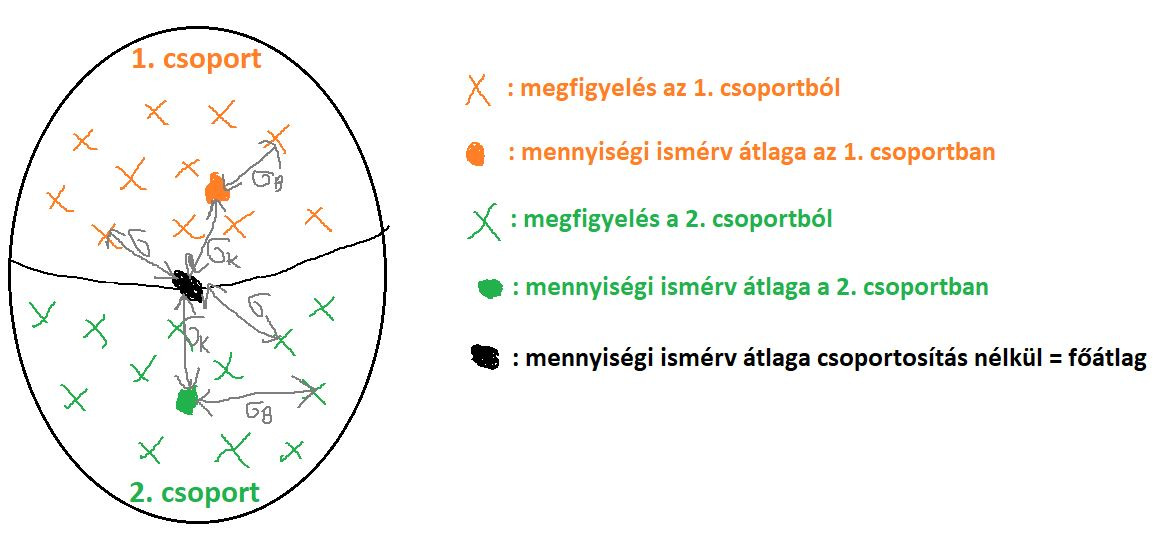
\includegraphics[width=0.8\textwidth,height=\textheight]{varhanyad1.jpg}

Tehát vizuálisan a következőképp érdemes gondolni a különböző \(\sigma\)-kra:

\begin{itemize}
\tightlist
\item
  \(\sigma_B\): Megfigyelések távolsága saját csoportjuk átlagától
\item
  \(\sigma_K\): Csoportátlag távolsága a főátlagtól
\item
  \(\sigma\): Megfigyelések távolsága a főátlagától
\end{itemize}

Ezek alapján nekünk az a jó a csoportosítás, azaz a minőségi ismérv magyarázóereje szempontjából, ha \textbf{fix} \(\sigma\) mellett \(\sigma_K\) \textbf{nagy} és \(\sigma_B\) \textbf{kicsi}. Mert ekkor a \textbf{csoportátlagok messze vannak} a főátlagtól és így implicite \textbf{egymástól} is, míg a csoportátlagtól az egyes \textbf{megfigyelések nagyon kis mértékben térnek csak el saját csoportátlaguktól}:

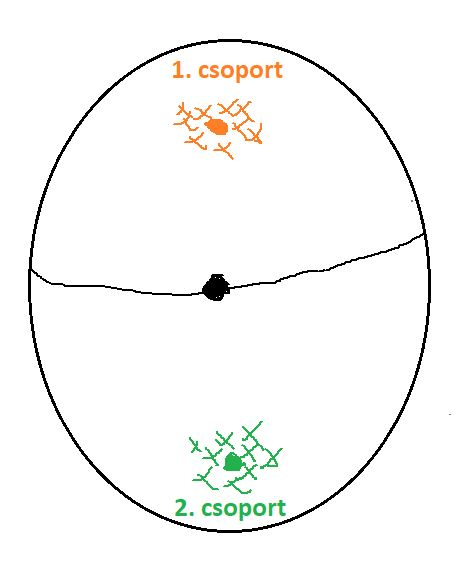
\includegraphics[width=0.3\textwidth,height=\textheight]{varhanyad2.jpg}

Ebben az esetben, ahogy az ábráról is látszik a csoportosításunk, azaz a minőségi ismérvünk magyarázóereje nagy! Tehát az kell nekünk, hogy az \(\sigma\) minél nagyobb részét tegye ki \(\sigma_K\). Viszont, mivel csak a teljes \textbf{varianciára} igaz az, hogy \textbf{egyenlő a külső és belső VARIANCIA összegével}, így azt mondjuk, hogy \textbf{azt szeretnénk látni}, hogy \textbf{a \(\frac{\sigma_K^2}{\sigma^2}\) hányados nagy legyen}! Ez a mutató lesz tehát a \textbf{varianciahányados}, és a most elvégzett módszer neve a \textbf{variancia-analízis, azaz ANOVA = ANalysis Of VAriances}.

\textbf{Azért a varianciákra néztük végül a dolgokat}, mert \(\sigma^2=\sigma_B^2+\sigma_K^2\), így a \(\frac{\sigma_K^2}{\sigma^2}\) variancia-hányados biztos, hogy \(0-1\) közötti, és \textbf{százalékosan} is értelmezhető, hiszen \(\sigma_K^2\) része \(\sigma^2\)-nek. Ez alapján nekünk most:

\(\frac{\sigma_K^2}{\sigma^2} = \frac{933.98387}{3996.64097}=0.23369=23.369\%\) --\textgreater{} \textbf{A hónap (tehát a Sound jelenléte) a Balatonban mért kokainmennyiség alakulásának (varianciájának) kb. 23\%-át magyarázza a megfigyelt adatok körében!} Ez egy \textbf{közepes magyarázóerő}nek tekinthető, mivel a variancia-hányadost a következőképpen ``\emph{korszakoljuk}'':

\begin{itemize}
\tightlist
\item
  \textbf{variancia-hányados \textless{} 10\% --\textgreater{} gyenge kapcsolat}
\item
  \textbf{10\% \textless= variancia-hányados \textless= 50\% --\textgreater{} közepes kapcsolat}
\item
  \textbf{variancia-hányados \textgreater{} 50\% --\textgreater{} erős/szoros kapcsolat}
\end{itemize}

\subsection{További minőségi ismérvek és a kokainmennyiség}\label{tovuxe1bbi-minux151suxe9gi-ismuxe9rvek-uxe9s-a-kokainmennyisuxe9g}

Az eredmény tehát azt mondja, hogy a kokainmennyiség alakulásának csak kb. \(23\%\)-át tudjuk csak lefedni azzal, hogy a mérés melyik hónapban készült. Tehát hónapkon \emph{belül} is jelentős mértékű szódósás maradt a mennyiségi ismérvünkben, jelesül a kokainmennyiségben.
Mi okozhatja még a kokainmennyiség szóródását? Hát, az elérhető adatok tekintetében két dolgot tudunk még megvizsgálni: azt, hogy \textbf{melyik mérőállomáson történt a mérés}, illetve azt, hogy \textbf{melyik évben}. Reméljük, hogy \emph{inkább az év magyarázza még relatíve nagyobb mértékben a kokainmennyiség alakulását} (pl. emelkedő trend tapasztalható a Sound népszerűségének növekedésével), mert \emph{ha a kokainmennyiség szóródása inkább a mérőállomástól függ}, az \emph{aggasztó lenne a mérés megbízhatóságára nézve}.

Mivel mind a mérőállomás azonosítója, mind az évszám jelen szituációban minőségi ismérvként kezelhető, így e két ismérvnek a kokainmennyiséggel, mint mennyiségi ismérvvel vett varianciahányadosát kell megvizsgálnunk.

Először nézzük a \textbf{mérőállomások esetét}.

Itt is kell ugyebár egy kiinduló segédtáblázat.

\begin{Shaded}
\begin{Highlighting}[]
\NormalTok{AllomasTabla }\OperatorTok{=}\NormalTok{ Balcsi.groupby(}\StringTok{\textquotesingle{}Allomas\textquotesingle{}}\NormalTok{).agg(}
\NormalTok{  Elemszam }\OperatorTok{=}\NormalTok{ (}\StringTok{\textquotesingle{}Kokain\textquotesingle{}}\NormalTok{, }\StringTok{\textquotesingle{}count\textquotesingle{}}\NormalTok{),}
\NormalTok{  Reszatlagok }\OperatorTok{=}\NormalTok{ (}\StringTok{\textquotesingle{}Kokain\textquotesingle{}}\NormalTok{, np.mean),}
\NormalTok{  Szorasok }\OperatorTok{=}\NormalTok{ (}\StringTok{\textquotesingle{}Kokain\textquotesingle{}}\NormalTok{, np.std)}
\NormalTok{).reset\_index()}
\end{Highlighting}
\end{Shaded}

\begin{verbatim}
## <string>:1: FutureWarning: The provided callable <function mean at 0x00000167D93F13A0> is currently using SeriesGroupBy.mean. In a future version of pandas, the provided callable will be used directly. To keep current behavior pass the string "mean" instead.
## <string>:1: FutureWarning: The provided callable <function std at 0x00000167D93F14E0> is currently using SeriesGroupBy.std. In a future version of pandas, the provided callable will be used directly. To keep current behavior pass the string "std" instead.
\end{verbatim}

\begin{Shaded}
\begin{Highlighting}[]
\NormalTok{AllomasTabla}
\end{Highlighting}
\end{Shaded}

\begin{verbatim}
##       Allomas  Elemszam  Reszatlagok   Szorasok
## 0  1. állomás       180    30.101843  84.544224
## 1  2. állomás       180    22.314141  61.220808
## 2  3. állomás       180    12.502428  30.877849
\end{verbatim}

Olybá tűnik, hogy az 1. állomás átlagban némileg kicsit magasabb kokainmenyniséget mér, mint a többi, de az állomás méréseinek szórása is magas, az átlagos kokainmennyiség kb. \(\frac{84.5}{30.1}=2.8\)-szorosa.
Szóval, vágjunk rendet a variancia-hányados segítségével, és lássuk mekkora hatást gyakorol a mérőállomás a kokainmennyiségre!

A számításokban annyi \textbf{egyszerűsítés}t teszek, hogy

\begin{itemize}
\tightlist
\item
  A \textbf{teljes varianciát örökítem} az előző számolásokból, hiszen az a csoportosítás alapját képzőú minőpségi ismérv megváltozásával \textbf{nem változik}.
\item
  Az előző pont és a belső variancia kiszámolása után pedig a varianciahányadost a \(\sigma^2=\sigma_B^2+\sigma_K^2\) összefüggás átrendezésével \(H^2=\frac{\sigma^2-\sigma_B^2}{\sigma^2}=1-\frac{\sigma_B^2}{\sigma^2}\) módon számolom ki
\end{itemize}

Ezzel a két módosítással \textbf{megúszom a külső szórásnégyzet} kissé macerás \textbf{kiszámítását}.

\begin{Shaded}
\begin{Highlighting}[]
\NormalTok{belső\_var\_Állomás }\OperatorTok{=}\NormalTok{ np.}\BuiltInTok{sum}\NormalTok{(AllomasTabla.Elemszam }\OperatorTok{*}\NormalTok{ AllomasTabla.Szorasok}\OperatorTok{**}\DecValTok{2}\NormalTok{)}\OperatorTok{/}\NormalTok{np.}\BuiltInTok{sum}\NormalTok{(AllomasTabla.Elemszam)}

\NormalTok{VarHányadÁllomás }\OperatorTok{=} \DecValTok{1} \OperatorTok{{-}}\NormalTok{ belső\_var\_Állomás }\OperatorTok{/}\NormalTok{ teljes\_var}
\NormalTok{VarHányadÁllomás}
\end{Highlighting}
\end{Shaded}

\begin{verbatim}
## 0.01174053573946432
\end{verbatim}

Az eredmény mindössze \(1.17\%\). Tehát megnyugodhatunk, az \textbf{állomás a mért kokainmennyiség alakulását csak alig több, mint 1\%-ban határozza meg}! A \textbf{mérés nem függ lényegében az állomástól}, így ilyen szempointból megbízhatónak tekintehtők!

Lássuk az \textbf{évszámok}at! Most is kezdjük a segédtáblával.

\begin{Shaded}
\begin{Highlighting}[]
\NormalTok{EvTabla }\OperatorTok{=}\NormalTok{ Balcsi.groupby(}\StringTok{\textquotesingle{}Ev\textquotesingle{}}\NormalTok{).agg(}
\NormalTok{  Elemszam }\OperatorTok{=}\NormalTok{ (}\StringTok{\textquotesingle{}Kokain\textquotesingle{}}\NormalTok{, }\StringTok{\textquotesingle{}count\textquotesingle{}}\NormalTok{),}
\NormalTok{  Reszatlagok }\OperatorTok{=}\NormalTok{ (}\StringTok{\textquotesingle{}Kokain\textquotesingle{}}\NormalTok{, np.mean),}
\NormalTok{  Szorasok }\OperatorTok{=}\NormalTok{ (}\StringTok{\textquotesingle{}Kokain\textquotesingle{}}\NormalTok{, np.std)}
\NormalTok{).reset\_index()}
\end{Highlighting}
\end{Shaded}

\begin{verbatim}
## <string>:1: FutureWarning: The provided callable <function mean at 0x00000167D93F13A0> is currently using SeriesGroupBy.mean. In a future version of pandas, the provided callable will be used directly. To keep current behavior pass the string "mean" instead.
## <string>:1: FutureWarning: The provided callable <function std at 0x00000167D93F14E0> is currently using SeriesGroupBy.std. In a future version of pandas, the provided callable will be used directly. To keep current behavior pass the string "std" instead.
\end{verbatim}

\begin{Shaded}
\begin{Highlighting}[]
\NormalTok{EvTabla}
\end{Highlighting}
\end{Shaded}

\begin{verbatim}
##      Ev  Elemszam  Reszatlagok   Szorasok
## 0  2017       180     0.536273   0.734331
## 1  2018       180     1.964270   3.933046
## 2  2019       180    62.417870  97.366788
\end{verbatim}

Itt azért elég látványos eltéréseket találunk! A 2019-es évben hatalmasat ugrott a Balatonban mérhető kokainmennyiség. A szórása is magas, de pl. relatíve nézve 2018-ban magasabb volt: 2018-ban a szórás durván kétszerese volt az átlagnak \(\frac{3.93}{1.96}\), míg 2019-ben csak durván másfélszerese \(\frac{97.37}{62.42}=1.56\). Szóval itt lehet még komolyabb magyarázóerő!
De ne találgassunk, hanem lássuk a varianciahányadost! A számolásnál megint alkalmazzuk az állomásoknál bevezetett két \textbf{egyszerűsítés}t!

\begin{Shaded}
\begin{Highlighting}[]
\NormalTok{belső\_var\_Év }\OperatorTok{=}\NormalTok{ np.}\BuiltInTok{sum}\NormalTok{(EvTabla.Elemszam }\OperatorTok{*}\NormalTok{ EvTabla.Szorasok}\OperatorTok{**}\DecValTok{2}\NormalTok{)}\OperatorTok{/}\NormalTok{np.}\BuiltInTok{sum}\NormalTok{(EvTabla.Elemszam)}

\NormalTok{VarHányadÉv }\OperatorTok{=} \DecValTok{1} \OperatorTok{{-}}\NormalTok{ belső\_var\_Év }\OperatorTok{/}\NormalTok{ teljes\_var}
\NormalTok{VarHányadÉv}
\end{Highlighting}
\end{Shaded}

\begin{verbatim}
## 0.20797660221119585
\end{verbatim}

Na, itt is egy közepes magyarázóerőnk van, kb. \(21\%\).

Tehát alapvetően a Balatonban mérhető kokainmennyiséget két \emph{közepes magyarázóerejű} dolog mozgatja nyáron:

\begin{itemize}
\tightlist
\item
  \textbf{Hónap}: A Balaton Sound hónapjában (július) átlagban valamivel több a kokain
\item
  \textbf{Év}: 2019-ben sokkal több az átlagos kokainmennyiség, feltehetően a Sound megnövekedett haza és külföldi népszerűsége miatt
\end{itemize}

Szerencsére a mérőállomás maga nem befolyásolja érdemben a mért kokain szóródását, így a mérések ilyen szempontból megbízhatóank tekinthetők!

  \bibliography{book.bib,packages.bib}

\end{document}
